\documentclass{article}
\newcommand{\final}{0}
% Change to 1 for final submission, all notes are suppressed

\usepackage[final]{template}
\usepackage[utf8]{inputenc} % allow utf-8 input
\usepackage[T1]{fontenc}    % use 8-bit T1 fonts
\usepackage{hyperref}       % hyperlinks
\usepackage{url}            % simple URL typesetting
\usepackage{booktabs}       % professional-quality tables
\usepackage{amsfonts}       % blackboard math symbols
\usepackage{nicefrac}       % compact symbols for 1/2, etc.
\usepackage{microtype}      % microtypography
\usepackage{epsfig}
\usepackage{color}
\usepackage{parskip}
\usepackage{ifthen}
\usepackage{float}
\usepackage{alltt}
\usepackage{amsmath}
\usepackage{amssymb}
\usepackage{amsthm}
\usepackage{newlfont} % for Box
\usepackage{floatflt}
\usepackage{wrapfig}
\usepackage{fixltx2e}
\usepackage{subcaption} % for subfloat
\usepackage{multirow}
%\usepackage[breaklinks=true,bookmarks=false]{hyperref}
\usepackage{cleveref}
\usepackage{algorithmic}
\usepackage[export]{adjustbox}
\usepackage{mathtools, cuted}
%\usepackage[ruled]{algorithm2e} % For algorithms
\usepackage{microtype}
\usepackage{graphicx}
\usepackage{hyperref}

% Attempt to make hyperref and algorithmic work together better:
\newcommand{\theHalgorithm}{\arabic{algorithm}}


\newcommand*\samethanks[1][\value{footnote}]{\footnotemark[#1]}
\def\textrightarrow{$\rightarrow$}
\newcommand{\pcline }{\rule{0in}{0.0in}    }  % Spacing for pseudo-code.
\newcommand{\pctab  }{\hspace{0.10in}      }  % Pseudo-code indentation.
\newcommand{\pcbigtab  }{\hspace{1.75in}    }  % Pseudo-code indentation.
\newcommand{\pcasgn }{\mbox{$\leftarrow$}  }  % Pseudo-code assignment operator
\newcommand{\pcomment}[1]{\mbox{// {\it #1}}}  % Pseudo-code comments.
\newcommand{\pckeyword}[1]{\mbox{{\bf #1}}}  % Pseudo-code keywords.
\newcommand{\pcspace}{\hspace{0.10in}}

\newcommand{\pcode}[1]{
    \footnotesize
    \vspace{-0.1in}
    \begin{minipage}{100in} % The width argument will be ignored:
                            % See lamport p. 99
    \begin{tabbing} \hspace{0.10in} \= \pctab \= \pctab \= \pctab \= \pcbigtab \= \\
        #1
    \end{tabbing}
    \end{minipage}
%    \vspace{0.15in}
    }
%
\renewcommand{\algorithmicrequire}{\textbf{Input:}}
\renewcommand{\algorithmicensure}{\textbf{Output:}}

\newcommand{\tabtextsize}{\small}
\newcommand{\figtext}[1]{{\footnotesize #1}}
\newcommand{\Caption}[2]{\caption[#1]{{\em #1} #2}}
\newcommand{\invisible}[1]{{\color{white} #1}}
\newcommand{\emacsquote}[1]{{``#1''}}

\definecolor{color1}{rgb}{0.7,0,0}
\definecolor{color2}{rgb}{0,0.4,0}
\definecolor{color3}{rgb}{0,0,0.8}
\newcommand{\zjy}[1]{{\color{color1} Jiayao Zhang: #1 $\qed$}}
\newcommand{\szh}[1]{{\color{color2} Zehao Su: #1 $\qed$}}
\newcommand{\lc}[1]{{\color{color3} Chen Liu: #1 $\qed$}}
\newcommand{\warning}[1]{{\it\color{red} #1}}
\newcommand{\note}[1]{{\it\color{blue} #1}}
\newcommand{\nothing}[1]{}
\newcommand{\passthrough}[1]{#1}
\definecolor{AudioColor}{rgb}{0.56,0.34,0.62}
\newcommand{\audio}[1]{{\color{AudioColor} Audio: #1}}

\newcommand{\psdraftboxDefault}{\psnodraftbox}

\definecolor{figred}{rgb}{1,0,0}
\definecolor{figgreen}{rgb}{0,0.6,0}
\definecolor{figblue}{rgb}{0,0,1}
\definecolor{figpink}{rgb}{1,0.63,0.63}

%\ifthenelse{\equal{\final}{1}}
%{
%\renewcommand{\zjy}[1]{}
%\renewcommand{\szh}[1]{}
%\renewcommand{\lc}[1]{}
%\renewcommand{\warning}[1]{}
%\renewcommand{\note}[1]{}
%}

\newcommand{\pseudocode}{Algorithm}
\floatstyle{plain}
\newfloat{algorithm}{tbhp}{lop}
\floatname{algorithm}{\pseudocode}

\newcommand{\filename}[1]{\url{#1}}
\newcommand{\foldername}[1]{\url{#1}}

\let\oldparagraph\paragraph
\newcommand{\passage}[1]{\oldparagraph{\textbf{#1}}}
\renewcommand{\paragraph}[1]{\oldparagraph{\textbf{#1}.}} % \liyi{keep/remove that end period depending on whether you want a paragraph title to end with a period}

\newcommand{\command}[1]{{\color{black}{\tt #1}}}

\ifdefined\email
\else
\newcommand{\email}[1]{\url{#1}}
\fi



% Calculus and Linear Algebra
\newcommand{\diff}{\mathrm{d}}
\newcommand{\pd}{\partial}
\newcommand{\grad}{\nabla}
\newcommand{\tr}{\operatorname{tr}}
\newcommand{\samplesym}{s}
\newcommand{\sample}{\samplesym{}}
\newcommand{\samplesetsym}{\mathcal{S}}
\newcommand{\sampleset}{\samplesetsym{}}
\newcommand{\sampleprime}{\samplesym^{\prime}{}}
\newcommand{\dist}{d}
\newcommand{\conflictdist}{r}
\newcommand{\union}{\oplus}
\newcommand{\failure}{f}
\newcommand{\assign}{\leftarrow}

% useful math symbols
\renewcommand{\Pr}{{\bf Pr}}
\newcommand{\Prx}{\mathop{\bf Pr\/}}
\newcommand{\Exp}{{\bf E}}
\newcommand{\Expx}{\mathop{\bf E\/}}
\newcommand{\Var}{{\bf Var}}
\newcommand{\Varx}{\mathop{\bf Var\/}}
\newcommand{\Cov}{{\bf Cov}}
\newcommand{\Covx}{\mathop{\bf Cov\/}}

% shortcuts for symbol names that are too long to type
\newcommand{\eps}{\epsilon}
\newcommand{\lam}{\lambda}
\newcommand{\la}{\langle}
\newcommand{\ra}{\rangle}
\newcommand{\wh}{\widehat}
\newcommand{\wt}{\widetilde}

% "blackboard-fonted" letters for the reals, naturals etc.
\newcommand{\sR}{\mathbb R}
\newcommand{\sN}{\mathbb N}
\newcommand{\sZ}{\mathbb Z}
\newcommand{\sF}{\mathbb F}
\newcommand{\sQ}{\mathbb Q}
\newcommand{\sC}{\mathbb C}


% calligraphic letters
\newcommand{\calA}{{\cal A}}
\newcommand{\calB}{{\cal B}}
\newcommand{\calC}{{\cal C}}
\newcommand{\calD}{{\cal D}}
\newcommand{\calE}{{\cal E}}
\newcommand{\calF}{{\cal F}}
\newcommand{\calG}{{\cal G}}
\newcommand{\calH}{{\cal H}}
\newcommand{\calI}{{\cal I}}
\newcommand{\calJ}{{\cal J}}
\newcommand{\calK}{{\cal K}}
\newcommand{\calL}{{\cal L}}
\newcommand{\calM}{{\cal M}}
\newcommand{\calN}{{\cal N}}
\newcommand{\calO}{{\cal O}}
\newcommand{\calP}{{\cal P}}
\newcommand{\calQ}{{\cal Q}}
\newcommand{\calR}{{\cal R}}
\newcommand{\calS}{{\cal S}}
\newcommand{\calT}{{\cal T}}
\newcommand{\calU}{{\cal U}}
\newcommand{\calV}{{\cal V}}
\newcommand{\calW}{{\cal W}}
\newcommand{\calX}{{\cal X}}
\newcommand{\calY}{{\cal Y}}
\newcommand{\calZ}{{\cal Z}}

% bold letters (useful for random variables)
\renewcommand{\a}{{\boldsymbol a}}
\renewcommand{\b}{{\boldsymbol b}}
\renewcommand{\c}{{\boldsymbol c}}
\renewcommand{\d}{{\boldsymbol d}}
\newcommand{\e}{{\boldsymbol e}}
\newcommand{\f}{{\boldsymbol f}}
\newcommand{\g}{{\boldsymbol g}}
\newcommand{\h}{{\boldsymbol h}}
\renewcommand{\i}{{\boldsymbol i}}
\renewcommand{\j}{{\boldsymbol j}}
\renewcommand{\k}{{\boldsymbol k}}
\renewcommand{\l}{{\boldsymbol l}}
\newcommand{\m}{{\boldsymbol m}}
\newcommand{\n}{{\boldsymbol n}}
\renewcommand{\o}{{\boldsymbol o}}
\newcommand{\p}{{\boldsymbol p}}
\newcommand{\q}{{\boldsymbol q}}
\renewcommand{\r}{{\boldsymbol r}}
\newcommand{\s}{{\boldsymbol s}}
\renewcommand{\t}{{\boldsymbol t}}
\renewcommand{\u}{{\boldsymbol u}}
\renewcommand{\v}{{\boldsymbol v}}
\newcommand{\w}{{\boldsymbol w}}
\newcommand{\x}{{\boldsymbol x}}
\newcommand{\y}{{\boldsymbol y}}
\newcommand{\z}{{\boldsymbol z}}
\newcommand{\A}{{\boldsymbol A}}
\newcommand{\B}{{\boldsymbol B}}
\newcommand{\C}{{\boldsymbol C}}
\newcommand{\D}{{\boldsymbol D}}
\newcommand{\E}{{\boldsymbol E}}
\newcommand{\F}{{\boldsymbol F}}
\newcommand{\G}{{\boldsymbol G}}
\renewcommand{\H}{{\boldsymbol H}}
\newcommand{\I}{{\boldsymbol I}}
\newcommand{\J}{{\boldsymbol J}}
\newcommand{\K}{{\boldsymbol K}}
\renewcommand{\L}{{\boldsymbol L}}
\newcommand{\M}{{\boldsymbol M}}
\newcommand{\N}{{\boldsymbol N}}
\renewcommand{\O}{{\boldsymbol O}}
\renewcommand{\P}{{\boldsymbol P}}
\newcommand{\Q}{{\boldsymbol Q}}
\newcommand{\R}{{\boldsymbol R}}
\renewcommand{\S}{{\boldsymbol S}}
\newcommand{\T}{{\boldsymbol T}}
\newcommand{\U}{{\boldsymbol U}}
\newcommand{\V}{{\boldsymbol V}}
\newcommand{\W}{{\boldsymbol W}}
\newcommand{\X}{{\boldsymbol X}}
\newcommand{\Y}{{\boldsymbol Y}}
\newcommand{\Z}{{\boldsymbol Z}}

\newcommand{\funct}[1]{\texttt{#1}}
\newcommand{\tp}[1]{#1 ^ {\top}}
\renewcommand{\Re}[1]{\mathfrak{Re}\left(#1\right)}
\renewcommand{\Im}[1]{\mathfrak{Im}\left(#1\right)}

\graphicspath{{figs/}}
\newcommand{\noun}[1]{\textbf{#1}}
\newcommand{\var}[1]{\texttt{#1}}
\title{Understanding Admission Results of CS Graduate Programs in U.S. Universities}

% hi guys, pls fill in the details
\author{
    Chen~Liu\thanks{Indicates equal contribution.},~~Zehao~Su\samethanks{},~~and~Jiayao~Zhang\samethanks{}\\
    University of Hong Kong\\
    Pokfulam, Hong Kong\\
    \texttt{\{liuchen,taylorsu,zjohnson\}@connect.hku.hk}\\
}

\begin{document}
\maketitle

\begin{abstract}
    Recent years have witnessed a surge in Computer Science (CS) research, which achieved unparalleled
    successes in a kaleidoscope of science and engineering applications spanning
    artificial intelligence \cite{Silver:2016:Go}, natural language processing \cite{Manning:2014:NLP}, computer vision \cite{Alex:2012:AlexNet},
    statistical learning theory \cite{LeCun:2015:DL}, blockchain and cryptocurrency \cite{Bonneau:2015:SOK},
    computational biology \cite{Cock:2009:BioPy} and bioinformatics \cite{Saeys:2007:Bio},
    intelligent grids and Internet-of-Things (IoT) \cite{Atzori:2010:IOT}. Consequently,
    the difficulty of pursuing a higher degree in CS or related subjects in decent graduate
    schools has been elevated to an unprecedented new height \cite{Rag:2010:GRAD}. In this paper, motivated
    by these observations, the authors, consisting of a data-driven earth scientist, a computational biologist,
     and a machine learning researcher, study the factors governing the
    admissions of graduate schools in the U.S. by means of \noun{general linear models} (GLM),
    \noun{general additive models} (GAM), \noun{nonparametric methods} such as ensemble learning and
    \noun{Discrete Bayesian Networks} (DBN).
    We seek answers to several interesting questions and
    render crisp insights from the model inference and analysis.
    We conclude this paper by providing guidelines for future graduate schools
    applicants, identifying limitations that are not addressed by this paper
    and pointing out several possible future directions.
\end{abstract}

\section{Introduction}

We study the admission results of applications for CS graduate school in the U.S. We obtain data from \noun{GradCafe} \cite{GradCafe} and
\noun{CSRankings} \cite{CSR}. In this paper, we study the factors governing the decision made through GLM and GAM, we compare the results
learnt through canonical nonparametric learning methods including ensemble methods and boosting. We further explore the dependency relationship
among the data by way of discrete Bayesian network.
Through the study outlined in this paper, we aim at seeking a better understanding of graduate school applications in CS related subjects. We summarize our contribution as follows:

\begin{itemize}
    \item We give a systematic study of the data available on \noun{GradCafe} \cite{GradCafe}.
	To the best of our knowledge, this is the first work achieving this.

    \item We give quantitative results of the answers to the following curious and important
	questions:
	    \begin{enumerate}
		\item \emph{What are the significant covariates that impact the application results?}

		\item \emph{Do GPA and standard test scores affects the application results differently for MS
		    and PhD applicants?}

		\item \emph{Does possessing a U.S. Bachelor degree significantly increases the likelihood of being admitted?}
	    \end{enumerate}

    \item We give guidelines and insights drawn from our analysis to prospective applicants.

\end{itemize}

This paper is structured as follows, \Cref{sec:background} introduces
the dataset protocol and recall important notions of GLM and GAM, which
we only give a brief treatment as the readers of this paper are expected
to be familiar with these topics; \Cref{sec:methods} discusses the models
we adopt for the admission results data, we emphasis on the applicability
and estimate the expressivity of the model chosen; we next fit the proposed
model in \Cref{sec:results} together with model selection and parameter analysis
and interpretation, based on which, we are ready to outline the answers to the
questions of interest as well as provide tips in \Cref{sec:conclusions}. We also
include a sketchy mention of the limitations and future directions as we
conclude this paper.


\section{Background on Data Acquisition and Exploration} \label{sec:background}

\begin{figure}[h]
    \centering
    \begin{subfigure}{.5\linewidth}\centering
	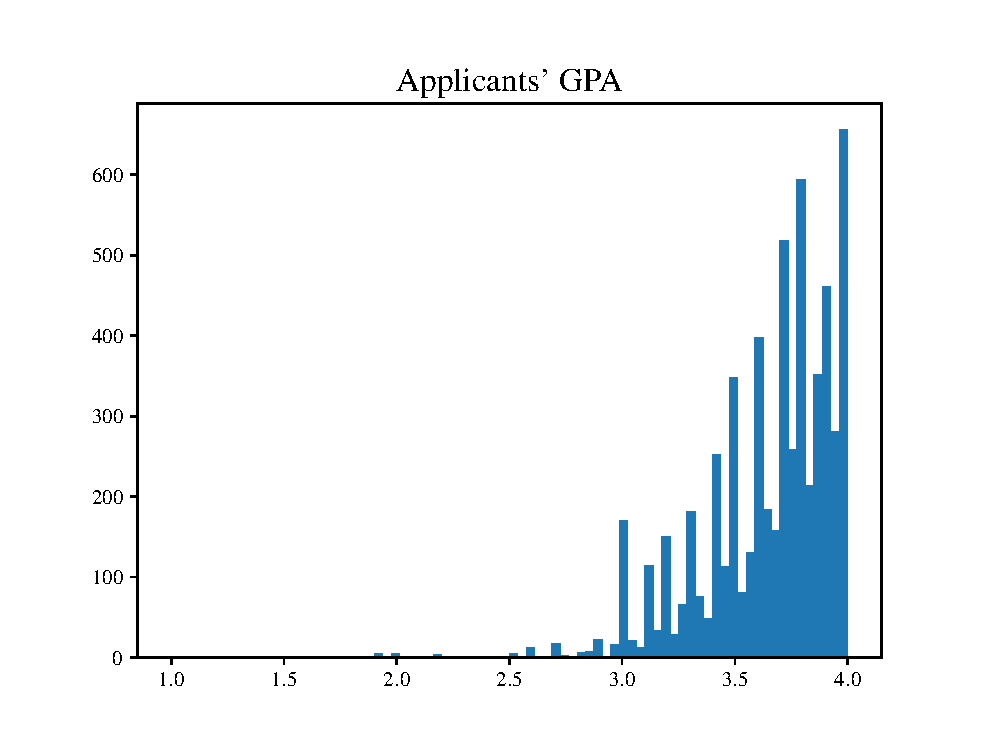
\includegraphics[width=\textwidth]{gpa.eps}
	\caption{Histogram of Applicants' GPA.}
    \end{subfigure}%
    \begin{subfigure}{.5\linewidth}\centering
	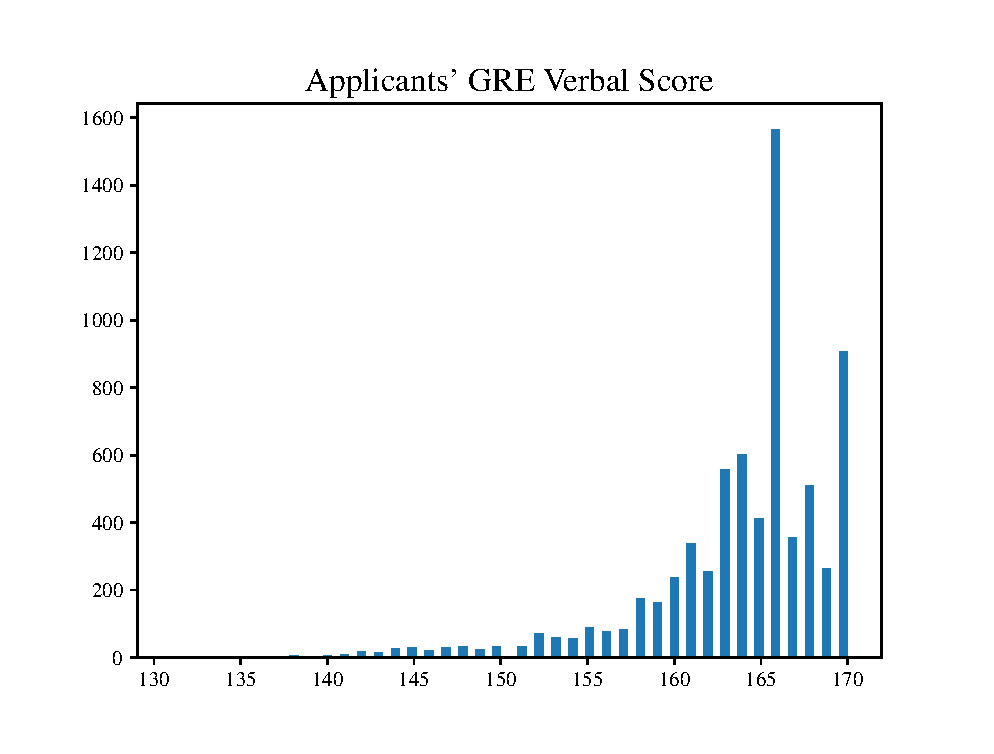
\includegraphics[width=\textwidth]{gre.eps}
	\caption{Histogram of Applicants' GRE Verbal Score.}
    \end{subfigure}
    \begin{subfigure}{.5\linewidth}\centering
	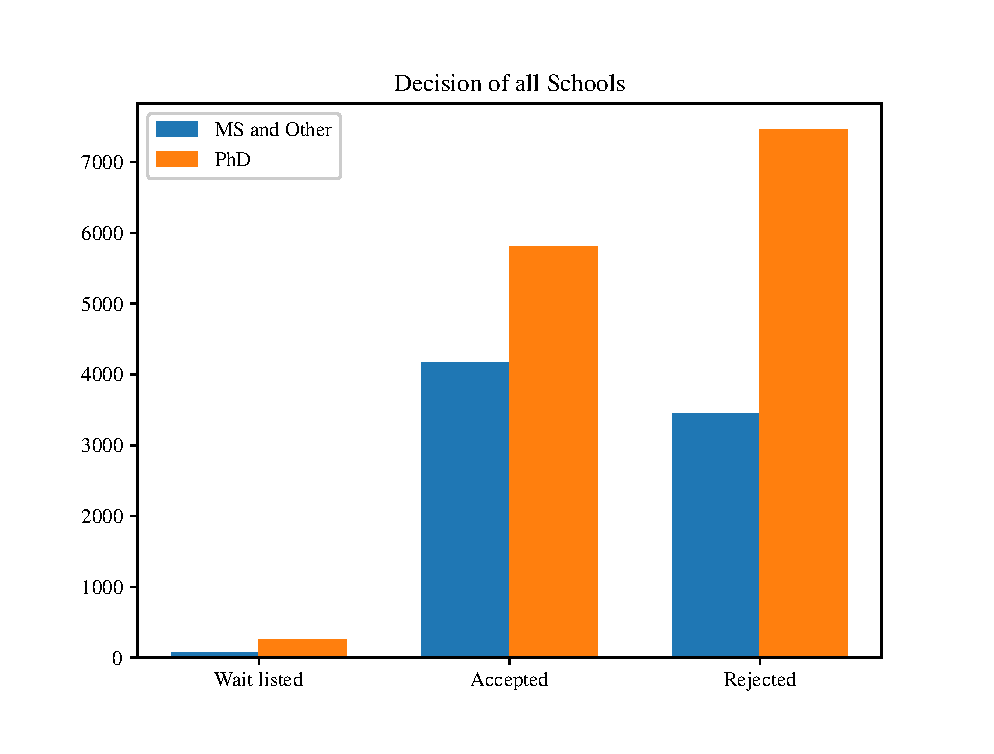
\includegraphics[width=\textwidth]{all_decision.eps}
	\caption{Overall Decisions.}
    \end{subfigure}%
    \begin{subfigure}{.5\linewidth}\centering
	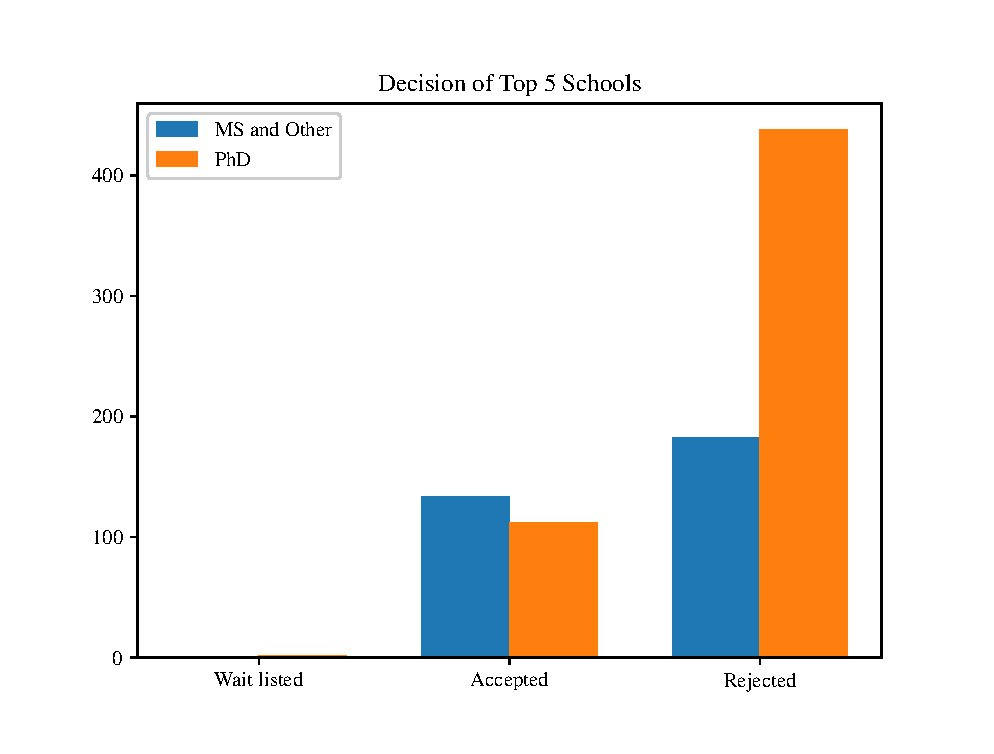
\includegraphics[width=\textwidth]{top5_decision.eps}
	\caption{Decisions from Top 5 Schools.}
    \end{subfigure}%
    \caption{Histograms of Selected Covariates.}  \label{fig:dataset}
\end{figure}

	\begin{table}[htpb]
	    \centering
	    \begin{tabular}{cccc}
		Institution & Program (Season) & Decision \& Date & Status \\\hline\hline
		\emph{Stanford University} & CS Masters (F18) & Rejected via E-mail on 16 March 2018 & I \\
		\multicolumn{4}{l}{Comment: \emph{I think I have no grad schools to attend next year.}}\\
		\emph{Stanford University} & CS PhD (F18) & Accepted via Phone on 7 Feb 2018 & U \\
		\multicolumn{4}{l}{Comment: \emph{Call from POI and email from student buddy. Absolutely shocked and very excited.}}\\
		\ldots\\
		\emph{UC Berkeley} & EECS PhD (F18) & Accepted via E-mail on 2 Feb 2018 & A \\
		\multicolumn{4}{l}{Comment: \emph{Accepted with nomination for university fellowship. 1 first author conference talk...}}\\ \hline\hline
	    \end{tabular}
	    \caption{Samples of \noun{GradCafe} dataset.}
	    \label{table:data_sample}
	\end{table}
	In this paper, we collect data from \noun{GradCafe} \cite{GradCafe}, an online
	sharing platform of graduate school admission results. The dataset
	involves the following covariates:
	\var{university}, the graduate school the applicant applied for;
	\var{degree}, one of either \var{\{MBA, MEng, MFA, MS, PhD, Other\}}, the desired degree applied for;
	\var{decision}, one of either \var{\{Accepted, Rejected, Wait Listed\}}, the application result;
	\var{gpa}, the latest Grading Point Average (GPA) the applicant possesses;
	\var{gre\_verbal}, \var{gre\_quant}, \var{gre\_writing}, standard test scores examining verbal, quantitative and writing skills;
	\var{status}, either one of \var{\{American, International, International with US Degree,
	Other\}}, dictating the status of the applicant as of the application
	\var{comments}, additional information shared by the applicant. Several
	typical entries are tabulated in \Cref{table:data_sample}.

	We augment this dataset by introducing metrics examining the prestigious of the graduate
	school. Instead of selecting from a variety of university ranking, we focus on the \noun{CSRanking} \cite{CSR},
	which is specifically tailored for CS research. To that end, we attach two more covariates per record,
	namely,
	\var{uni\_pub}, the university publication index as the multiplier of number of total publications with reference
	to the lowest value;
	\var{faculty}, the number of faculty members (not counting Emeritus faculties).
	We note through our data exploration, these metrics, though may seem partial at first mention,
	are consistent with the general college ranking results such as
	the US News and Times.

	We preprocess the dataset to select those applications made to US universities,
	clean up invalid data, normalize the GPA on a $4.0$ scale and GRE tests
	to new scale ($170$ maximum). We also merge the categories \var{\{MBA, MEng, MFA, MS, Other\}}
	to a singleton \var{MS} as it suffices the objectives set for this paper. After these manipulations,
	we had $21209$ records from the applications ranging from $2011$ to $2015$. Noted some records
	may miss certain metrics such as GPA, in that case, our model ignore the very entries for parameter
	estimation. A short summary of the cleaned dataset is given in \Cref{table:data_summary:quant,table:data_summary:cat}. We also plot the histogram of several selected covariates in \Cref{fig:dataset}.

	\begin{table}[htpb]
	    \centering
	    \begin{tabular}{|c|c|c|c|c|c|}
		\hline
		Covariate & Available Record & Min. & Mean & Median & Max. \\\hline
		\var{gpa} & $6015$ & $1.00$ & $3.65$ & $3.70$ & $4.00$ \\\hline
		\var{gre\_verbal} & $7078$ & $130.0$ & $157.8$ & $158.0$ & $170.0$ \\\hline
		\var{gre\_quant} & $7078$ & $131.0$ & $163.9$ & $166.0$ & $170.0$ \\\hline
		\var{gre\_writing} & $6873$ & $2.00$ & $3.89$ & $4.00$ & $6.00$ \\\hline
		\var{uni\_pub} & all & $1.00$ & $6.38$ & $5.40$ & $18.10$ \\\hline
		\var{faculty} & all & $2$ & $53$ & $50$ & $152$ \\\hline
	    \end{tabular}
	    \caption{Summary for Quantitative Covariates.}
	    \label{table:data_summary:quant}
	\end{table}

	\begin{table}[htpb]
	    \centering
	    \begin{subtable}{0.2\textwidth}\centering
	    \begin{tabular}{|c|c|}
		\hline
		MS & PhD \\\hline
		7693 & 13516 \\\hline
	    \end{tabular}
		\caption{\var{degree}.}
	    \end{subtable}%
	    \begin{subtable}{0.4\textwidth}\centering
	    \begin{tabular}{|c|c|c|}
		\hline
		Accepted & Rejected & Wait Listed \\\hline
		9971 & 10912 & 326 \\\hline
	    \end{tabular}
		\caption{\var{decision}.}
	    \end{subtable}%
	    \begin{subtable}{0.4\textwidth}\centering
	    \begin{tabular}{|c|c|c|c|}
		\hline
		A & U & I & O \\\hline
		4159 & 2747 & 13546 & 219 \\\hline
	    \end{tabular}
		\caption{\var{status}.}
	    \end{subtable}
	    \caption{Summary for Categorical Covariates.}
	    \label{table:data_summary:cat}
	\end{table}
	
\section{Generalized Additive Model} \label{sec:gam}
In this section, we explore one of the most intuitive methods of fitting a binary-response data set. General additive models (GAM) are a natural extension of generalized linear models (GLM), which accept response(s) distributed as a member of the exponential family through the use of link function, by allowing covariates to be modeled with both parametric specifications and nonparametric techniques. Predictors \texttt{degree}, \texttt{decision\_method}, \texttt{decision\_month}, \texttt{gre}, \texttt{status}, \texttt{uni\_faclty} and \texttt{uni\_pub} are used in this section. A derived variable, \texttt{gre}, is constructed by addition of \texttt{gre\_quant}, \texttt{gre\_verbal} and \texttt{gre\_writing}, based on the assumption that final decisions made may be related to the overall score only.
\subsection{Logistic Regression}
To start with, we consider tje canonical logistic regression, whose performance, evaluated by the area under the \noun{Receiver Operating Characteristic Curve} (AUC), will be regarded as a benchmark in this paper. The value of AUC ranges from 0 to 1, depending on the discriminating power of each model. A larger AUC value indicates better separation of the data, while a value equal to 0.5 implies the model does no better than simply tossing a coin.
\par Parameterization of a good-old logistic regression model is specified below.
\begin{align}
\log\left(\frac{p}{1-p}\right)=\mathbf{x}^\top\boldsymbol{\beta}+\beta_0
\end{align}
where $p=P(Y=1)$ is the probability of the candidate being accepted by the school, and $\mathbf{x}$ is a vector of predictors, which can be either numerical and categorical. 
\par Forward selection is a greedy approach of variable selection by including one independent variable which helps explain the most deviance. This procedure, based on Alkaike's Information Criteria (AIC), measures goodness-of-fit using a penalized maximum likelihood, imposing greater penalty on models with higher complexity. The result suggests a model including all predictors (AIC=5574.28).
\par One may also be interested in whether the two types of degrees have different requirements or selection criteria for candidates with the same academic merits and/or applying under the same category. Based on this motivation, three interaction effects (\texttt{degree:status}, \texttt{degree:gpa} and \texttt{degree:gre}) are consequently added to the model fitted above. However, only \texttt{degree:status} has a significant effect under 5\% level of significance. The inclusion of such effect can be further supported by the AIC statistic, which is brought down to 5570.2. The AUC on test data set is evaluated as 0.716.

\subsection{The Lasso}
Now we approach the variable selection problem again with another popular method, the Lasso \cite{Friedman:2001:ESL}, which is a shrinkage method of the regression coefficients by putting a constraint on the $L_1$-norm of $\boldsymbol{\beta}$. The parameter estimate can be written as the solution to an optimization problem.
\begin{align}
\widehat{\boldsymbol{\beta}}^{\text{lasso}}=\underset{\boldsymbol{\beta}}{\arg\min}\left\{\sum_i\left[\log\left(\frac{p_i}{1-p_i}\right)-\mathbf{x}^\top\boldsymbol{\beta}-\beta_0\right]^2+\lambda\|\boldsymbol{\beta}\|_1\right\}
\end{align}
where $\lambda$ controls the extent to which the regression coefficients are suppressed. In particular, the lasso, as opposed to ridge regression with penalty laid on the $L_2$-norm, has a variable selection power. \Cref{lassopath} shows the regularization path of $\boldsymbol{\beta}$ along its corresponding $L_1$-norm, where each line represents the numerical value of regression coefficient of one predictor. The optimal choice of $\lambda$ is attained by 5-fold cross valication (CV) scheme, whose binomial deviance lies upper one standard error of the minimum choice, as shown in \Cref{lassocv}.

\begin{figure}[tpb]
  \centering
    \begin{subfigure}[t]{.5\textwidth} \centering
	\resizebox{\textwidth}{!}{%
	% Created by tikzDevice version 0.11 on 2018-04-28 11:50:00
% !TEX encoding = UTF-8 Unicode
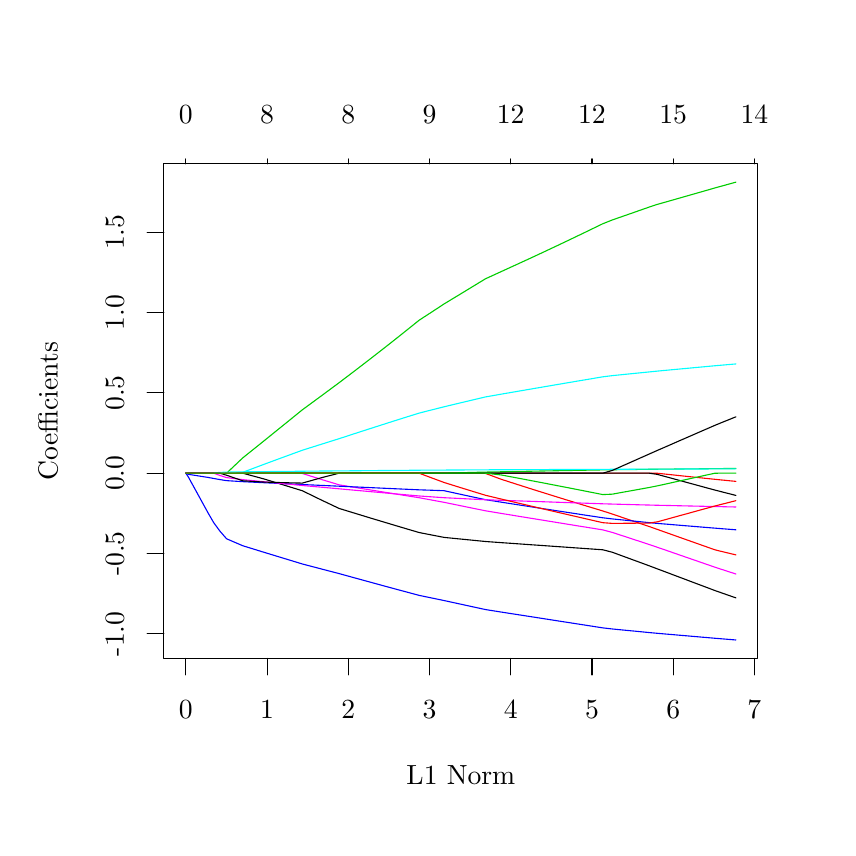
\begin{tikzpicture}[x=1pt,y=1pt]
\definecolor{fillColor}{RGB}{255,255,255}
\path[use as bounding box,fill=fillColor,fill opacity=0.00] (0,0) rectangle (289.08,289.08);
\begin{scope}
\path[clip] ( 49.20, 61.20) rectangle (263.88,239.88);
\definecolor{drawColor}{RGB}{0,0,0}

\path[draw=drawColor,line width= 0.4pt,line join=round,line cap=round] ( 57.15,128.09) --
	( 58.01,128.09) --
	( 60.63,128.09) --
	( 63.01,128.09) --
	( 65.19,128.09) --
	( 67.23,128.09) --
	( 69.45,128.09) --
	( 71.87,128.09) --
	( 77.71,128.09) --
	( 85.35,126.02) --
	( 92.54,123.81) --
	( 99.24,121.75) --
	(106.13,118.39) --
	(112.54,115.35) --
	(118.27,113.60) --
	(123.60,111.97) --
	(128.56,110.48) --
	(133.17,109.10) --
	(137.46,107.82) --
	(141.45,106.65) --
	(146.13,105.73) --
	(150.48,104.89) --
	(155.79,104.36) --
	(160.75,103.87) --
	(165.40,103.41) --
	(171.18,102.99) --
	(176.64,102.61) --
	(181.69,102.25) --
	(186.37,101.93) --
	(190.69,101.62) --
	(194.69,101.34) --
	(198.37,101.08) --
	(201.78,100.84) --
	(204.91,100.62) --
	(207.80,100.42) --
	(211.24, 99.53) --
	(215.01, 98.14) --
	(218.48, 96.87) --
	(221.67, 95.70) --
	(224.61, 94.62) --
	(227.46, 93.54) --
	(230.42, 92.44) --
	(233.18, 91.39) --
	(235.68, 90.45) --
	(237.97, 89.59) --
	(240.10, 88.78) --
	(242.02, 88.06) --
	(243.80, 87.39) --
	(245.41, 86.79) --
	(246.87, 86.24) --
	(248.23, 85.72) --
	(249.52, 85.27) --
	(250.72, 84.85) --
	(251.79, 84.48) --
	(252.74, 84.14) --
	(253.66, 83.82) --
	(254.50, 83.53) --
	(255.23, 83.27) --
	(255.93, 83.03);
\end{scope}
\begin{scope}
\path[clip] (  0.00,  0.00) rectangle (289.08,289.08);
\definecolor{drawColor}{RGB}{0,0,0}

\path[draw=drawColor,line width= 0.4pt,line join=round,line cap=round] ( 57.15, 61.20) -- (262.60, 61.20);

\path[draw=drawColor,line width= 0.4pt,line join=round,line cap=round] ( 57.15, 61.20) -- ( 57.15, 55.20);

\path[draw=drawColor,line width= 0.4pt,line join=round,line cap=round] ( 86.50, 61.20) -- ( 86.50, 55.20);

\path[draw=drawColor,line width= 0.4pt,line join=round,line cap=round] (115.85, 61.20) -- (115.85, 55.20);

\path[draw=drawColor,line width= 0.4pt,line join=round,line cap=round] (145.20, 61.20) -- (145.20, 55.20);

\path[draw=drawColor,line width= 0.4pt,line join=round,line cap=round] (174.55, 61.20) -- (174.55, 55.20);

\path[draw=drawColor,line width= 0.4pt,line join=round,line cap=round] (203.90, 61.20) -- (203.90, 55.20);

\path[draw=drawColor,line width= 0.4pt,line join=round,line cap=round] (233.25, 61.20) -- (233.25, 55.20);

\path[draw=drawColor,line width= 0.4pt,line join=round,line cap=round] (262.60, 61.20) -- (262.60, 55.20);

\node[text=drawColor,anchor=base,inner sep=0pt, outer sep=0pt, scale=  1.00] at ( 57.15, 39.60) {0};

\node[text=drawColor,anchor=base,inner sep=0pt, outer sep=0pt, scale=  1.00] at ( 86.50, 39.60) {1};

\node[text=drawColor,anchor=base,inner sep=0pt, outer sep=0pt, scale=  1.00] at (115.85, 39.60) {2};

\node[text=drawColor,anchor=base,inner sep=0pt, outer sep=0pt, scale=  1.00] at (145.20, 39.60) {3};

\node[text=drawColor,anchor=base,inner sep=0pt, outer sep=0pt, scale=  1.00] at (174.55, 39.60) {4};

\node[text=drawColor,anchor=base,inner sep=0pt, outer sep=0pt, scale=  1.00] at (203.90, 39.60) {5};

\node[text=drawColor,anchor=base,inner sep=0pt, outer sep=0pt, scale=  1.00] at (233.25, 39.60) {6};

\node[text=drawColor,anchor=base,inner sep=0pt, outer sep=0pt, scale=  1.00] at (262.60, 39.60) {7};

\path[draw=drawColor,line width= 0.4pt,line join=round,line cap=round] ( 49.20, 70.03) -- ( 49.20,215.18);

\path[draw=drawColor,line width= 0.4pt,line join=round,line cap=round] ( 49.20, 70.03) -- ( 43.20, 70.03);

\path[draw=drawColor,line width= 0.4pt,line join=round,line cap=round] ( 49.20, 99.06) -- ( 43.20, 99.06);

\path[draw=drawColor,line width= 0.4pt,line join=round,line cap=round] ( 49.20,128.09) -- ( 43.20,128.09);

\path[draw=drawColor,line width= 0.4pt,line join=round,line cap=round] ( 49.20,157.12) -- ( 43.20,157.12);

\path[draw=drawColor,line width= 0.4pt,line join=round,line cap=round] ( 49.20,186.15) -- ( 43.20,186.15);

\path[draw=drawColor,line width= 0.4pt,line join=round,line cap=round] ( 49.20,215.18) -- ( 43.20,215.18);

\node[text=drawColor,rotate= 90.00,anchor=base,inner sep=0pt, outer sep=0pt, scale=  1.00] at ( 34.80, 70.03) {-1.0};

\node[text=drawColor,rotate= 90.00,anchor=base,inner sep=0pt, outer sep=0pt, scale=  1.00] at ( 34.80, 99.06) {-0.5};

\node[text=drawColor,rotate= 90.00,anchor=base,inner sep=0pt, outer sep=0pt, scale=  1.00] at ( 34.80,128.09) {0.0};

\node[text=drawColor,rotate= 90.00,anchor=base,inner sep=0pt, outer sep=0pt, scale=  1.00] at ( 34.80,157.12) {0.5};

\node[text=drawColor,rotate= 90.00,anchor=base,inner sep=0pt, outer sep=0pt, scale=  1.00] at ( 34.80,186.15) {1.0};

\node[text=drawColor,rotate= 90.00,anchor=base,inner sep=0pt, outer sep=0pt, scale=  1.00] at ( 34.80,215.18) {1.5};

\path[draw=drawColor,line width= 0.4pt,line join=round,line cap=round] ( 49.20, 61.20) --
	(263.88, 61.20) --
	(263.88,239.88) --
	( 49.20,239.88) --
	( 49.20, 61.20);
\end{scope}
\begin{scope}
\path[clip] (  0.00,  0.00) rectangle (289.08,289.08);
\definecolor{drawColor}{RGB}{0,0,0}

\node[text=drawColor,anchor=base,inner sep=0pt, outer sep=0pt, scale=  1.00] at (156.54, 15.60) {L1 Norm};

\node[text=drawColor,rotate= 90.00,anchor=base,inner sep=0pt, outer sep=0pt, scale=  1.00] at ( 10.80,150.54) {Coefficients};
\end{scope}
\begin{scope}
\path[clip] ( 49.20, 61.20) rectangle (263.88,239.88);
\definecolor{drawColor}{RGB}{255,0,0}

\path[draw=drawColor,line width= 0.4pt,line join=round,line cap=round] ( 57.15,128.09) --
	( 58.01,128.09) --
	( 60.63,128.09) --
	( 63.01,128.09) --
	( 65.19,128.09) --
	( 67.23,128.09) --
	( 69.45,128.09) --
	( 71.87,128.09) --
	( 77.71,128.09) --
	( 85.35,128.09) --
	( 92.54,128.09) --
	( 99.24,128.09) --
	(106.13,128.09) --
	(112.54,128.09) --
	(118.27,128.09) --
	(123.60,128.09) --
	(128.56,128.09) --
	(133.17,128.09) --
	(137.46,128.09) --
	(141.45,128.09) --
	(146.13,128.09) --
	(150.48,128.09) --
	(155.79,128.09) --
	(160.75,128.09) --
	(165.40,128.09) --
	(171.18,128.09) --
	(176.64,128.09) --
	(181.69,128.09) --
	(186.37,128.09) --
	(190.69,128.09) --
	(194.69,128.09) --
	(198.37,128.09) --
	(201.78,128.09) --
	(204.91,128.09) --
	(207.80,128.09) --
	(211.24,128.09) --
	(215.01,128.09) --
	(218.48,128.09) --
	(221.67,128.09) --
	(224.61,128.09) --
	(227.46,128.08) --
	(230.42,127.76) --
	(233.18,127.47) --
	(235.68,127.20) --
	(237.97,126.96) --
	(240.10,126.74) --
	(242.02,126.53) --
	(243.80,126.35) --
	(245.41,126.18) --
	(246.87,126.03) --
	(248.23,125.89) --
	(249.52,125.76) --
	(250.72,125.64) --
	(251.79,125.54) --
	(252.74,125.44) --
	(253.66,125.35) --
	(254.50,125.27) --
	(255.23,125.20) --
	(255.93,125.13);
\definecolor{drawColor}{RGB}{0,205,0}

\path[draw=drawColor,line width= 0.4pt,line join=round,line cap=round] ( 57.15,128.09) --
	( 58.01,128.09) --
	( 60.63,128.09) --
	( 63.01,128.09) --
	( 65.19,128.09) --
	( 67.23,128.09) --
	( 69.45,128.09) --
	( 71.87,128.09) --
	( 77.71,133.61) --
	( 85.35,139.74) --
	( 92.54,145.55) --
	( 99.24,150.98) --
	(106.13,156.04) --
	(112.54,160.79) --
	(118.27,165.14) --
	(123.60,169.24) --
	(128.56,173.10) --
	(133.17,176.73) --
	(137.46,180.15) --
	(141.45,183.36) --
	(146.13,186.40) --
	(150.48,189.26) --
	(155.79,192.47) --
	(160.75,195.49) --
	(165.40,198.32) --
	(171.18,200.97) --
	(176.64,203.47) --
	(181.69,205.79) --
	(186.37,207.97) --
	(190.69,210.00) --
	(194.69,211.90) --
	(198.37,213.66) --
	(201.78,215.30) --
	(204.91,216.82) --
	(207.80,218.22) --
	(211.24,219.59) --
	(215.01,220.90) --
	(218.48,222.11) --
	(221.67,223.23) --
	(224.61,224.26) --
	(227.46,225.20) --
	(230.42,226.04) --
	(233.18,226.82) --
	(235.68,227.54) --
	(237.97,228.19) --
	(240.10,228.80) --
	(242.02,229.35) --
	(243.80,229.86) --
	(245.41,230.32) --
	(246.87,230.74) --
	(248.23,231.14) --
	(249.52,231.49) --
	(250.72,231.82) --
	(251.79,232.11) --
	(252.74,232.38) --
	(253.66,232.63) --
	(254.50,232.86) --
	(255.23,233.07) --
	(255.93,233.26);
\definecolor{drawColor}{RGB}{0,0,255}

\path[draw=drawColor,line width= 0.4pt,line join=round,line cap=round] ( 57.15,128.09) --
	( 58.01,126.80) --
	( 60.63,122.04) --
	( 63.01,117.70) --
	( 65.19,113.73) --
	( 67.23,110.20) --
	( 69.45,107.18) --
	( 71.87,104.39) --
	( 77.71,101.88) --
	( 85.35, 99.52) --
	( 92.54, 97.33) --
	( 99.24, 95.29) --
	(106.13, 93.48) --
	(112.54, 91.81) --
	(118.27, 90.23) --
	(123.60, 88.77) --
	(128.56, 87.41) --
	(133.17, 86.16) --
	(137.46, 85.01) --
	(141.45, 83.94) --
	(146.13, 82.97) --
	(150.48, 82.07) --
	(155.79, 80.91) --
	(160.75, 79.83) --
	(165.40, 78.82) --
	(171.18, 77.90) --
	(176.64, 77.05) --
	(181.69, 76.27) --
	(186.37, 75.54) --
	(190.69, 74.86) --
	(194.69, 74.24) --
	(198.37, 73.67) --
	(201.78, 73.14) --
	(204.91, 72.65) --
	(207.80, 72.20) --
	(211.24, 71.80) --
	(215.01, 71.43) --
	(218.48, 71.10) --
	(221.67, 70.79) --
	(224.61, 70.50) --
	(227.46, 70.24) --
	(230.42, 69.98) --
	(233.18, 69.75) --
	(235.68, 69.53) --
	(237.97, 69.34) --
	(240.10, 69.15) --
	(242.02, 68.99) --
	(243.80, 68.83) --
	(245.41, 68.70) --
	(246.87, 68.57) --
	(248.23, 68.45) --
	(249.52, 68.35) --
	(250.72, 68.25) --
	(251.79, 68.16) --
	(252.74, 68.08) --
	(253.66, 68.01) --
	(254.50, 67.94) --
	(255.23, 67.88) --
	(255.93, 67.82);
\definecolor{drawColor}{RGB}{0,255,255}

\path[draw=drawColor,line width= 0.4pt,line join=round,line cap=round] ( 57.15,128.09) --
	( 58.01,128.09) --
	( 60.63,128.09) --
	( 63.01,128.09) --
	( 65.19,128.09) --
	( 67.23,128.09) --
	( 69.45,128.09) --
	( 71.87,128.09) --
	( 77.71,128.41) --
	( 85.35,131.28) --
	( 92.54,133.93) --
	( 99.24,136.38) --
	(106.13,138.55) --
	(112.54,140.56) --
	(118.27,142.43) --
	(123.60,144.15) --
	(128.56,145.74) --
	(133.17,147.21) --
	(137.46,148.56) --
	(141.45,149.80) --
	(146.13,150.99) --
	(150.48,152.09) --
	(155.79,153.36) --
	(160.75,154.54) --
	(165.40,155.64) --
	(171.18,156.66) --
	(176.64,157.60) --
	(181.69,158.47) --
	(186.37,159.27) --
	(190.69,160.01) --
	(194.69,160.69) --
	(198.37,161.32) --
	(201.78,161.89) --
	(204.91,162.42) --
	(207.80,162.91) --
	(211.24,163.34) --
	(215.01,163.72) --
	(218.48,164.07) --
	(221.67,164.39) --
	(224.61,164.68) --
	(227.46,164.97) --
	(230.42,165.25) --
	(233.18,165.51) --
	(235.68,165.74) --
	(237.97,165.95) --
	(240.10,166.15) --
	(242.02,166.33) --
	(243.80,166.49) --
	(245.41,166.64) --
	(246.87,166.78) --
	(248.23,166.90) --
	(249.52,167.02) --
	(250.72,167.12) --
	(251.79,167.21) --
	(252.74,167.30) --
	(253.66,167.38) --
	(254.50,167.45) --
	(255.23,167.51) --
	(255.93,167.57);
\definecolor{drawColor}{RGB}{255,0,255}

\path[draw=drawColor,line width= 0.4pt,line join=round,line cap=round] ( 57.15,128.09) --
	( 58.01,128.09) --
	( 60.63,128.09) --
	( 63.01,128.09) --
	( 65.19,128.09) --
	( 67.23,128.09) --
	( 69.45,128.09) --
	( 71.87,128.09) --
	( 77.71,128.09) --
	( 85.35,128.09) --
	( 92.54,128.09) --
	( 99.24,128.00) --
	(106.13,125.83) --
	(112.54,123.88) --
	(118.27,122.94) --
	(123.60,122.08) --
	(128.56,121.28) --
	(133.17,120.54) --
	(137.46,119.86) --
	(141.45,119.23) --
	(146.13,118.36) --
	(150.48,117.56) --
	(155.79,116.47) --
	(160.75,115.45) --
	(165.40,114.51) --
	(171.18,113.55) --
	(176.64,112.65) --
	(181.69,111.83) --
	(186.37,111.07) --
	(190.69,110.37) --
	(194.69,109.72) --
	(198.37,109.12) --
	(201.78,108.58) --
	(204.91,108.07) --
	(207.80,107.61) --
	(211.24,106.69) --
	(215.01,105.46) --
	(218.48,104.32) --
	(221.67,103.28) --
	(224.61,102.32) --
	(227.46,101.34) --
	(230.42,100.33) --
	(233.18, 99.37) --
	(235.68, 98.50) --
	(237.97, 97.71) --
	(240.10, 96.97) --
	(242.02, 96.31) --
	(243.80, 95.69) --
	(245.41, 95.13) --
	(246.87, 94.63) --
	(248.23, 94.15) --
	(249.52, 93.73) --
	(250.72, 93.34) --
	(251.79, 93.00) --
	(252.74, 92.69) --
	(253.66, 92.39) --
	(254.50, 92.12) --
	(255.23, 91.88) --
	(255.93, 91.65);
\definecolor{drawColor}{RGB}{0,0,0}

\path[draw=drawColor,line width= 0.4pt,line join=round,line cap=round] ( 57.15,128.09) --
	( 58.01,128.09) --
	( 60.63,128.09) --
	( 63.01,128.09) --
	( 65.19,128.09) --
	( 67.23,128.09) --
	( 69.45,128.09) --
	( 71.87,128.09) --
	( 77.71,128.09) --
	( 85.35,128.09) --
	( 92.54,128.09) --
	( 99.24,128.09) --
	(106.13,128.09) --
	(112.54,128.09) --
	(118.27,128.09) --
	(123.60,128.09) --
	(128.56,128.09) --
	(133.17,128.09) --
	(137.46,128.09) --
	(141.45,128.09) --
	(146.13,128.09) --
	(150.48,128.09) --
	(155.79,128.09) --
	(160.75,128.09) --
	(165.40,128.09) --
	(171.18,128.09) --
	(176.64,128.09) --
	(181.69,128.09) --
	(186.37,128.09) --
	(190.69,128.09) --
	(194.69,128.09) --
	(198.37,128.09) --
	(201.78,128.09) --
	(204.91,128.09) --
	(207.80,128.09) --
	(211.24,128.09) --
	(215.01,128.09) --
	(218.48,128.09) --
	(221.67,128.09) --
	(224.61,128.09) --
	(227.46,127.67) --
	(230.42,126.87) --
	(233.18,126.12) --
	(235.68,125.44) --
	(237.97,124.81) --
	(240.10,124.23) --
	(242.02,123.71) --
	(243.80,123.22) --
	(245.41,122.78) --
	(246.87,122.39) --
	(248.23,122.02) --
	(249.52,121.69) --
	(250.72,121.38) --
	(251.79,121.11) --
	(252.74,120.87) --
	(253.66,120.63) --
	(254.50,120.42) --
	(255.23,120.23) --
	(255.93,120.05);
\definecolor{drawColor}{RGB}{255,0,0}

\path[draw=drawColor,line width= 0.4pt,line join=round,line cap=round] ( 57.15,128.09) --
	( 58.01,128.09) --
	( 60.63,128.09) --
	( 63.01,128.09) --
	( 65.19,128.09) --
	( 67.23,128.09) --
	( 69.45,128.09) --
	( 71.87,128.09) --
	( 77.71,128.09) --
	( 85.35,128.09) --
	( 92.54,128.09) --
	( 99.24,128.09) --
	(106.13,128.09) --
	(112.54,128.09) --
	(118.27,128.09) --
	(123.60,128.09) --
	(128.56,128.09) --
	(133.17,128.09) --
	(137.46,128.09) --
	(141.45,128.09) --
	(146.13,128.09) --
	(150.48,128.09) --
	(155.79,128.09) --
	(160.75,128.09) --
	(165.40,128.02) --
	(171.18,125.87) --
	(176.64,124.11) --
	(181.69,122.50) --
	(186.37,121.03) --
	(190.69,119.68) --
	(194.69,118.44) --
	(198.37,117.31) --
	(201.78,116.27) --
	(204.91,115.32) --
	(207.80,114.45) --
	(211.24,113.33) --
	(215.01,112.05) --
	(218.48,110.88) --
	(221.67,109.80) --
	(224.61,108.81) --
	(227.46,107.80) --
	(230.42,106.75) --
	(233.18,105.77) --
	(235.68,104.88) --
	(237.97,104.07) --
	(240.10,103.32) --
	(242.02,102.64) --
	(243.80,102.00) --
	(245.41,101.44) --
	(246.87,100.92) --
	(248.23,100.44) --
	(249.52,100.10) --
	(250.72, 99.82) --
	(251.79, 99.56) --
	(252.74, 99.33) --
	(253.66, 99.11) --
	(254.50, 98.91) --
	(255.23, 98.73) --
	(255.93, 98.57);
\definecolor{drawColor}{RGB}{0,205,0}

\path[draw=drawColor,line width= 0.4pt,line join=round,line cap=round] ( 57.15,128.09) --
	( 58.01,128.09) --
	( 60.63,128.09) --
	( 63.01,128.09) --
	( 65.19,128.09) --
	( 67.23,128.09) --
	( 69.45,128.09) --
	( 71.87,128.09) --
	( 77.71,128.09) --
	( 85.35,128.09) --
	( 92.54,128.09) --
	( 99.24,128.09) --
	(106.13,128.09) --
	(112.54,128.09) --
	(118.27,128.09) --
	(123.60,128.09) --
	(128.56,128.09) --
	(133.17,128.09) --
	(137.46,128.09) --
	(141.45,128.09) --
	(146.13,128.09) --
	(150.48,128.10) --
	(155.79,128.24) --
	(160.75,128.37) --
	(165.40,128.49) --
	(171.18,128.60) --
	(176.64,128.71) --
	(181.69,128.80) --
	(186.37,128.89) --
	(190.69,128.97) --
	(194.69,129.04) --
	(198.37,129.11) --
	(201.78,129.17) --
	(204.91,129.23) --
	(207.80,129.28) --
	(211.24,129.33) --
	(215.01,129.38) --
	(218.48,129.42) --
	(221.67,129.46) --
	(224.61,129.50) --
	(227.46,129.53) --
	(230.42,129.56) --
	(233.18,129.58) --
	(235.68,129.61) --
	(237.97,129.63) --
	(240.10,129.65) --
	(242.02,129.67) --
	(243.80,129.69) --
	(245.41,129.71) --
	(246.87,129.72) --
	(248.23,129.73) --
	(249.52,129.75) --
	(250.72,129.76) --
	(251.79,129.77) --
	(252.74,129.78) --
	(253.66,129.78) --
	(254.50,129.79) --
	(255.23,129.80) --
	(255.93,129.81);
\definecolor{drawColor}{RGB}{0,0,255}

\path[draw=drawColor,line width= 0.4pt,line join=round,line cap=round] ( 57.15,128.09) --
	( 58.01,127.69) --
	( 60.63,127.28) --
	( 63.01,126.90) --
	( 65.19,126.56) --
	( 67.23,126.18) --
	( 69.45,125.78) --
	( 71.87,125.40) --
	( 77.71,125.03) --
	( 85.35,124.65) --
	( 92.54,124.31) --
	( 99.24,123.99) --
	(106.13,123.68) --
	(112.54,123.39) --
	(118.27,123.13) --
	(123.60,122.89) --
	(128.56,122.66) --
	(133.17,122.45) --
	(137.46,122.26) --
	(141.45,122.08) --
	(146.13,121.92) --
	(150.48,121.76) --
	(155.79,120.60) --
	(160.75,119.52) --
	(165.40,118.53) --
	(171.18,117.61) --
	(176.64,116.76) --
	(181.69,115.98) --
	(186.37,115.25) --
	(190.69,114.59) --
	(194.69,113.98) --
	(198.37,113.42) --
	(201.78,112.89) --
	(204.91,112.42) --
	(207.80,111.98) --
	(211.24,111.57) --
	(215.01,111.19) --
	(218.48,110.84) --
	(221.67,110.52) --
	(224.61,110.22) --
	(227.46,109.95) --
	(230.42,109.71) --
	(233.18,109.48) --
	(235.68,109.27) --
	(237.97,109.08) --
	(240.10,108.91) --
	(242.02,108.75) --
	(243.80,108.60) --
	(245.41,108.47) --
	(246.87,108.35) --
	(248.23,108.24) --
	(249.52,108.14) --
	(250.72,108.04) --
	(251.79,107.96) --
	(252.74,107.88) --
	(253.66,107.81) --
	(254.50,107.75) --
	(255.23,107.69) --
	(255.93,107.63);
\definecolor{drawColor}{RGB}{0,255,255}

\path[draw=drawColor,line width= 0.4pt,line join=round,line cap=round] ( 57.15,128.09) --
	( 58.01,128.09) --
	( 60.63,128.09) --
	( 63.01,128.09) --
	( 65.19,128.09) --
	( 67.23,128.22) --
	( 69.45,128.36) --
	( 71.87,128.48) --
	( 77.71,128.58) --
	( 85.35,128.66) --
	( 92.54,128.73) --
	( 99.24,128.80) --
	(106.13,128.87) --
	(112.54,128.92) --
	(118.27,128.97) --
	(123.60,129.02) --
	(128.56,129.06) --
	(133.17,129.10) --
	(137.46,129.13) --
	(141.45,129.17) --
	(146.13,129.19) --
	(150.48,129.22) --
	(155.79,129.25) --
	(160.75,129.28) --
	(165.40,129.31) --
	(171.18,129.33) --
	(176.64,129.36) --
	(181.69,129.38) --
	(186.37,129.40) --
	(190.69,129.41) --
	(194.69,129.43) --
	(198.37,129.45) --
	(201.78,129.46) --
	(204.91,129.47) --
	(207.80,129.48) --
	(211.24,129.50) --
	(215.01,129.51) --
	(218.48,129.53) --
	(221.67,129.54) --
	(224.61,129.55) --
	(227.46,129.57) --
	(230.42,129.57) --
	(233.18,129.58) --
	(235.68,129.59) --
	(237.97,129.60) --
	(240.10,129.60) --
	(242.02,129.61) --
	(243.80,129.62) --
	(245.41,129.62) --
	(246.87,129.63) --
	(248.23,129.63) --
	(249.52,129.63) --
	(250.72,129.64) --
	(251.79,129.64) --
	(252.74,129.64) --
	(253.66,129.65) --
	(254.50,129.65) --
	(255.23,129.65) --
	(255.93,129.65);
\definecolor{drawColor}{RGB}{255,0,255}

\path[draw=drawColor,line width= 0.4pt,line join=round,line cap=round] ( 57.15,128.09) --
	( 58.01,128.09) --
	( 60.63,128.09) --
	( 63.01,128.09) --
	( 65.19,128.09) --
	( 67.23,128.08) --
	( 69.45,127.27) --
	( 71.87,126.50) --
	( 77.71,125.76) --
	( 85.35,125.01) --
	( 92.54,124.30) --
	( 99.24,123.64) --
	(106.13,123.03) --
	(112.54,122.45) --
	(118.27,121.93) --
	(123.60,121.45) --
	(128.56,121.01) --
	(133.17,120.59) --
	(137.46,120.21) --
	(141.45,119.86) --
	(146.13,119.53) --
	(150.48,119.23) --
	(155.79,118.97) --
	(160.75,118.72) --
	(165.40,118.49) --
	(171.18,118.29) --
	(176.64,118.10) --
	(181.69,117.93) --
	(186.37,117.77) --
	(190.69,117.62) --
	(194.69,117.48) --
	(198.37,117.35) --
	(201.78,117.24) --
	(204.91,117.13) --
	(207.80,117.03) --
	(211.24,116.93) --
	(215.01,116.83) --
	(218.48,116.74) --
	(221.67,116.65) --
	(224.61,116.58) --
	(227.46,116.50) --
	(230.42,116.44) --
	(233.18,116.38) --
	(235.68,116.32) --
	(237.97,116.27) --
	(240.10,116.22) --
	(242.02,116.18) --
	(243.80,116.14) --
	(245.41,116.10) --
	(246.87,116.07) --
	(248.23,116.04) --
	(249.52,116.01) --
	(250.72,115.99) --
	(251.79,115.97) --
	(252.74,115.94) --
	(253.66,115.93) --
	(254.50,115.91) --
	(255.23,115.89) --
	(255.93,115.88);
\definecolor{drawColor}{RGB}{0,0,0}

\path[draw=drawColor,line width= 0.4pt,line join=round,line cap=round] ( 57.15,128.09) --
	( 58.01,128.09) --
	( 60.63,128.09) --
	( 63.01,128.09) --
	( 65.19,128.09) --
	( 67.23,128.09) --
	( 69.45,128.09) --
	( 71.87,127.35) --
	( 77.71,125.35) --
	( 85.35,124.88) --
	( 92.54,124.66) --
	( 99.24,124.51) --
	(106.13,126.45) --
	(112.54,128.09) --
	(118.27,128.09) --
	(123.60,128.09) --
	(128.56,128.09) --
	(133.17,128.09) --
	(137.46,128.09) --
	(141.45,128.09) --
	(146.13,128.09) --
	(150.48,128.09) --
	(155.79,128.09) --
	(160.75,128.09) --
	(165.40,128.09) --
	(171.18,128.09) --
	(176.64,128.09) --
	(181.69,128.09) --
	(186.37,128.09) --
	(190.69,128.09) --
	(194.69,128.09) --
	(198.37,128.09) --
	(201.78,128.09) --
	(204.91,128.09) --
	(207.80,128.09) --
	(211.24,129.08) --
	(215.01,130.76) --
	(218.48,132.30) --
	(221.67,133.72) --
	(224.61,135.02) --
	(227.46,136.29) --
	(230.42,137.57) --
	(233.18,138.78) --
	(235.68,139.88) --
	(237.97,140.87) --
	(240.10,141.80) --
	(242.02,142.64) --
	(243.80,143.42) --
	(245.41,144.11) --
	(246.87,144.75) --
	(248.23,145.34) --
	(249.52,145.87) --
	(250.72,146.36) --
	(251.79,146.79) --
	(252.74,147.17) --
	(253.66,147.54) --
	(254.50,147.89) --
	(255.23,148.18) --
	(255.93,148.46);
\definecolor{drawColor}{RGB}{255,0,0}

\path[draw=drawColor,line width= 0.4pt,line join=round,line cap=round] ( 57.15,128.09) --
	( 58.01,128.09) --
	( 60.63,128.09) --
	( 63.01,128.09) --
	( 65.19,128.09) --
	( 67.23,128.09) --
	( 69.45,128.09) --
	( 71.87,128.09) --
	( 77.71,128.09) --
	( 85.35,128.09) --
	( 92.54,128.09) --
	( 99.24,128.09) --
	(106.13,128.09) --
	(112.54,128.09) --
	(118.27,128.09) --
	(123.60,128.09) --
	(128.56,128.09) --
	(133.17,128.09) --
	(137.46,128.09) --
	(141.45,128.09) --
	(146.13,126.34) --
	(150.48,124.73) --
	(155.79,123.07) --
	(160.75,121.54) --
	(165.40,120.12) --
	(171.18,118.73) --
	(176.64,117.44) --
	(181.69,116.25) --
	(186.37,115.16) --
	(190.69,114.15) --
	(194.69,113.23) --
	(198.37,112.38) --
	(201.78,111.59) --
	(204.91,110.87) --
	(207.80,110.21) --
	(211.24,109.95) --
	(215.01,109.98) --
	(218.48,110.01) --
	(221.67,110.04) --
	(224.61,110.07) --
	(227.46,110.50) --
	(230.42,111.30) --
	(233.18,112.07) --
	(235.68,112.76) --
	(237.97,113.38) --
	(240.10,113.97) --
	(242.02,114.50) --
	(243.80,114.99) --
	(245.41,115.43) --
	(246.87,115.83) --
	(248.23,116.21) --
	(249.52,116.54) --
	(250.72,116.85) --
	(251.79,117.11) --
	(252.74,117.35) --
	(253.66,117.58) --
	(254.50,117.80) --
	(255.23,117.98) --
	(255.93,118.16);
\definecolor{drawColor}{RGB}{0,205,0}

\path[draw=drawColor,line width= 0.4pt,line join=round,line cap=round] ( 57.15,128.09) --
	( 58.01,128.09) --
	( 60.63,128.09) --
	( 63.01,128.09) --
	( 65.19,128.09) --
	( 67.23,128.09) --
	( 69.45,128.09) --
	( 71.87,128.09) --
	( 77.71,128.09) --
	( 85.35,128.09) --
	( 92.54,128.09) --
	( 99.24,128.09) --
	(106.13,128.09) --
	(112.54,128.09) --
	(118.27,128.09) --
	(123.60,128.09) --
	(128.56,128.09) --
	(133.17,128.09) --
	(137.46,128.09) --
	(141.45,128.09) --
	(146.13,128.09) --
	(150.48,128.09) --
	(155.79,128.09) --
	(160.75,128.09) --
	(165.40,128.09) --
	(171.18,127.44) --
	(176.64,126.41) --
	(181.69,125.45) --
	(186.37,124.56) --
	(190.69,123.72) --
	(194.69,122.95) --
	(198.37,122.23) --
	(201.78,121.56) --
	(204.91,120.94) --
	(207.80,120.36) --
	(211.24,120.51) --
	(215.01,121.20) --
	(218.48,121.82) --
	(221.67,122.40) --
	(224.61,122.93) --
	(227.46,123.50) --
	(230.42,124.14) --
	(233.18,124.76) --
	(235.68,125.31) --
	(237.97,125.81) --
	(240.10,126.28) --
	(242.02,126.70) --
	(243.80,127.10) --
	(245.41,127.45) --
	(246.87,127.76) --
	(248.23,128.06) --
	(249.52,128.09) --
	(250.72,128.09) --
	(251.79,128.09) --
	(252.74,128.09) --
	(253.66,128.09) --
	(254.50,128.09) --
	(255.23,128.09) --
	(255.93,128.09);
\end{scope}
\begin{scope}
\path[clip] (  0.00,  0.00) rectangle (289.08,289.08);
\definecolor{drawColor}{RGB}{0,0,0}

\path[draw=drawColor,line width= 0.4pt,line join=round,line cap=round] ( 57.15,239.88) -- (262.60,239.88);

\path[draw=drawColor,line width= 0.4pt,line join=round,line cap=round] ( 57.15,239.88) -- ( 57.15,241.67);

\path[draw=drawColor,line width= 0.4pt,line join=round,line cap=round] ( 86.50,239.88) -- ( 86.50,241.67);

\path[draw=drawColor,line width= 0.4pt,line join=round,line cap=round] (115.85,239.88) -- (115.85,241.67);

\path[draw=drawColor,line width= 0.4pt,line join=round,line cap=round] (145.20,239.88) -- (145.20,241.67);

\path[draw=drawColor,line width= 0.4pt,line join=round,line cap=round] (174.55,239.88) -- (174.55,241.67);

\path[draw=drawColor,line width= 0.4pt,line join=round,line cap=round] (203.90,239.88) -- (203.90,241.67);

\path[draw=drawColor,line width= 0.4pt,line join=round,line cap=round] (233.25,239.88) -- (233.25,241.67);

\path[draw=drawColor,line width= 0.4pt,line join=round,line cap=round] (262.60,239.88) -- (262.60,241.67);

\node[text=drawColor,anchor=base,inner sep=0pt, outer sep=0pt, scale=  1.00] at ( 57.15,254.28) {0};

\node[text=drawColor,anchor=base,inner sep=0pt, outer sep=0pt, scale=  1.00] at ( 86.50,254.28) {8};

\node[text=drawColor,anchor=base,inner sep=0pt, outer sep=0pt, scale=  1.00] at (115.85,254.28) {8};

\node[text=drawColor,anchor=base,inner sep=0pt, outer sep=0pt, scale=  1.00] at (145.20,254.28) {9};

\node[text=drawColor,anchor=base,inner sep=0pt, outer sep=0pt, scale=  1.00] at (174.55,254.28) {12};

\node[text=drawColor,anchor=base,inner sep=0pt, outer sep=0pt, scale=  1.00] at (203.90,254.28) {12};

\node[text=drawColor,anchor=base,inner sep=0pt, outer sep=0pt, scale=  1.00] at (233.25,254.28) {15};

\node[text=drawColor,anchor=base,inner sep=0pt, outer sep=0pt, scale=  1.00] at (262.60,254.28) {14};
\end{scope}
\end{tikzpicture}
}
	\caption{Regularization path of the Lasso. Lines with different colours correspond to different covariates.} \label{lassopath}
    \end{subfigure}%
    \begin{subfigure}[t]{.5\textwidth} \centering
	\resizebox{\textwidth}{!}{%
	    % Created by tikzDevice version 0.11 on 2018-04-28 11:50:00
% !TEX encoding = UTF-8 Unicode
\begin{tikzpicture}[x=1pt,y=1pt]
\definecolor{fillColor}{RGB}{255,255,255}
\path[use as bounding box,fill=fillColor,fill opacity=0.00] (0,0) rectangle (289.08,289.08);
\begin{scope}
\path[clip] (  0.00,  0.00) rectangle (289.08,289.08);
\definecolor{drawColor}{RGB}{0,0,0}

\path[draw=drawColor,line width= 0.4pt,line join=round,line cap=round] ( 49.71, 61.20) -- (110.95, 61.20);

\path[draw=drawColor,line width= 0.4pt,line join=round,line cap=round] ( 49.71, 61.20) -- ( 49.71, 55.20);

\path[draw=drawColor,line width= 0.4pt,line join=round,line cap=round] ( 61.96, 61.20) -- ( 61.96, 55.20);

\path[draw=drawColor,line width= 0.4pt,line join=round,line cap=round] ( 74.21, 61.20) -- ( 74.21, 55.20);

\path[draw=drawColor,line width= 0.4pt,line join=round,line cap=round] ( 86.45, 61.20) -- ( 86.45, 55.20);

\path[draw=drawColor,line width= 0.4pt,line join=round,line cap=round] ( 98.70, 61.20) -- ( 98.70, 55.20);

\path[draw=drawColor,line width= 0.4pt,line join=round,line cap=round] (110.95, 61.20) -- (110.95, 55.20);

\node[text=drawColor,anchor=base,inner sep=0pt, outer sep=0pt, scale=  1.00] at ( 49.71, 39.60) {-8};

\node[text=drawColor,anchor=base,inner sep=0pt, outer sep=0pt, scale=  1.00] at ( 74.21, 39.60) {-6};

\node[text=drawColor,anchor=base,inner sep=0pt, outer sep=0pt, scale=  1.00] at ( 98.70, 39.60) {-4};

\path[draw=drawColor,line width= 0.4pt,line join=round,line cap=round] ( 49.20, 85.92) -- ( 49.20,197.88);

\path[draw=drawColor,line width= 0.4pt,line join=round,line cap=round] ( 49.20, 85.92) -- ( 43.20, 85.92);

\path[draw=drawColor,line width= 0.4pt,line join=round,line cap=round] ( 49.20,141.90) -- ( 43.20,141.90);

\path[draw=drawColor,line width= 0.4pt,line join=round,line cap=round] ( 49.20,197.88) -- ( 43.20,197.88);

\node[text=drawColor,rotate= 90.00,anchor=base,inner sep=0pt, outer sep=0pt, scale=  1.00] at ( 34.80, 85.92) {1.25};

\node[text=drawColor,rotate= 90.00,anchor=base,inner sep=0pt, outer sep=0pt, scale=  1.00] at ( 34.80,141.90) {1.30};

\node[text=drawColor,rotate= 90.00,anchor=base,inner sep=0pt, outer sep=0pt, scale=  1.00] at ( 34.80,197.88) {1.35};

\path[draw=drawColor,line width= 0.4pt,line join=round,line cap=round] ( 49.20, 61.20) --
	(119.34, 61.20) --
	(119.34,239.88) --
	( 49.20,239.88) --
	( 49.20, 61.20);
\end{scope}
\begin{scope}
\path[clip] (  0.00,  0.00) rectangle (144.54,289.08);
\definecolor{drawColor}{RGB}{0,0,0}

\node[text=drawColor,anchor=base,inner sep=0pt, outer sep=0pt, scale=  1.00] at ( 84.27, 15.60) {log(Lambda)};

\node[text=drawColor,rotate= 90.00,anchor=base,inner sep=0pt, outer sep=0pt, scale=  1.00] at ( 10.80,150.54) {Binomial Deviance};
\end{scope}
\begin{scope}
\path[clip] ( 49.20, 61.20) rectangle (119.34,239.88);
\definecolor{drawColor}{RGB}{169,169,169}

\path[draw=drawColor,line width= 0.4pt,line join=round,line cap=round] (116.74,233.26) -- (116.74,229.06);

\path[draw=drawColor,line width= 0.4pt,line join=round,line cap=round] (115.60,226.74) -- (115.60,223.35);

\path[draw=drawColor,line width= 0.4pt,line join=round,line cap=round] (114.46,218.56) -- (114.46,214.50);

\path[draw=drawColor,line width= 0.4pt,line join=round,line cap=round] (113.32,210.99) -- (113.32,206.41);

\path[draw=drawColor,line width= 0.4pt,line join=round,line cap=round] (112.18,204.56) -- (112.18,199.49);

\path[draw=drawColor,line width= 0.4pt,line join=round,line cap=round] (111.05,196.33) -- (111.05,190.84);

\path[draw=drawColor,line width= 0.4pt,line join=round,line cap=round] (109.91,187.74) -- (109.91,181.46);

\path[draw=drawColor,line width= 0.4pt,line join=round,line cap=round] (108.77,179.23) -- (108.77,172.31);

\path[draw=drawColor,line width= 0.4pt,line join=round,line cap=round] (107.63,170.42) -- (107.63,163.03);

\path[draw=drawColor,line width= 0.4pt,line join=round,line cap=round] (106.49,161.26) -- (106.49,153.59);

\path[draw=drawColor,line width= 0.4pt,line join=round,line cap=round] (105.35,153.23) -- (105.35,145.19);

\path[draw=drawColor,line width= 0.4pt,line join=round,line cap=round] (104.21,146.20) -- (104.21,137.38);

\path[draw=drawColor,line width= 0.4pt,line join=round,line cap=round] (103.07,140.14) -- (103.07,130.57);

\path[draw=drawColor,line width= 0.4pt,line join=round,line cap=round] (101.93,135.04) -- (101.93,124.83);

\path[draw=drawColor,line width= 0.4pt,line join=round,line cap=round] (100.79,130.58) -- (100.79,120.02);

\path[draw=drawColor,line width= 0.4pt,line join=round,line cap=round] ( 99.65,126.68) -- ( 99.65,115.98);

\path[draw=drawColor,line width= 0.4pt,line join=round,line cap=round] ( 98.51,123.47) -- ( 98.51,112.56);

\path[draw=drawColor,line width= 0.4pt,line join=round,line cap=round] ( 97.37,120.85) -- ( 97.37,109.67);

\path[draw=drawColor,line width= 0.4pt,line join=round,line cap=round] ( 96.23,118.65) -- ( 96.23,107.21);

\path[draw=drawColor,line width= 0.4pt,line join=round,line cap=round] ( 95.09,116.80) -- ( 95.09,105.11);

\path[draw=drawColor,line width= 0.4pt,line join=round,line cap=round] ( 93.95,115.25) -- ( 93.95,103.31);

\path[draw=drawColor,line width= 0.4pt,line join=round,line cap=round] ( 92.82,113.31) -- ( 92.82,100.96);

\path[draw=drawColor,line width= 0.4pt,line join=round,line cap=round] ( 91.68,109.47) -- ( 91.68, 97.29);

\path[draw=drawColor,line width= 0.4pt,line join=round,line cap=round] ( 90.54,105.19) -- ( 90.54, 92.92);

\path[draw=drawColor,line width= 0.4pt,line join=round,line cap=round] ( 89.40,101.53) -- ( 89.40, 89.13);

\path[draw=drawColor,line width= 0.4pt,line join=round,line cap=round] ( 88.26, 98.47) -- ( 88.26, 85.92);

\path[draw=drawColor,line width= 0.4pt,line join=round,line cap=round] ( 87.12, 95.92) -- ( 87.12, 83.18);

\path[draw=drawColor,line width= 0.4pt,line join=round,line cap=round] ( 85.98, 93.80) -- ( 85.98, 80.85);

\path[draw=drawColor,line width= 0.4pt,line join=round,line cap=round] ( 84.84, 92.05) -- ( 84.84, 78.88);

\path[draw=drawColor,line width= 0.4pt,line join=round,line cap=round] ( 83.70, 90.60) -- ( 83.70, 77.23);

\path[draw=drawColor,line width= 0.4pt,line join=round,line cap=round] ( 82.56, 89.40) -- ( 82.56, 75.83);

\path[draw=drawColor,line width= 0.4pt,line join=round,line cap=round] ( 81.42, 88.42) -- ( 81.42, 74.64);

\path[draw=drawColor,line width= 0.4pt,line join=round,line cap=round] ( 80.28, 87.62) -- ( 80.28, 73.64);

\path[draw=drawColor,line width= 0.4pt,line join=round,line cap=round] ( 79.14, 86.97) -- ( 79.14, 72.80);

\path[draw=drawColor,line width= 0.4pt,line join=round,line cap=round] ( 78.00, 86.43) -- ( 78.00, 72.04);

\path[draw=drawColor,line width= 0.4pt,line join=round,line cap=round] ( 76.86, 85.91) -- ( 76.86, 71.34);

\path[draw=drawColor,line width= 0.4pt,line join=round,line cap=round] ( 75.72, 85.46) -- ( 75.72, 70.70);

\path[draw=drawColor,line width= 0.4pt,line join=round,line cap=round] ( 74.59, 85.10) -- ( 74.59, 70.17);

\path[draw=drawColor,line width= 0.4pt,line join=round,line cap=round] ( 73.45, 84.71) -- ( 73.45, 69.71);

\path[draw=drawColor,line width= 0.4pt,line join=round,line cap=round] ( 72.31, 84.38) -- ( 72.31, 69.32);

\path[draw=drawColor,line width= 0.4pt,line join=round,line cap=round] ( 71.17, 84.11) -- ( 71.17, 69.00);

\path[draw=drawColor,line width= 0.4pt,line join=round,line cap=round] ( 70.03, 83.90) -- ( 70.03, 68.74);

\path[draw=drawColor,line width= 0.4pt,line join=round,line cap=round] ( 68.89, 83.74) -- ( 68.89, 68.53);

\path[draw=drawColor,line width= 0.4pt,line join=round,line cap=round] ( 67.75, 83.60) -- ( 67.75, 68.35);

\path[draw=drawColor,line width= 0.4pt,line join=round,line cap=round] ( 66.61, 83.50) -- ( 66.61, 68.21);

\path[draw=drawColor,line width= 0.4pt,line join=round,line cap=round] ( 65.47, 83.41) -- ( 65.47, 68.09);

\path[draw=drawColor,line width= 0.4pt,line join=round,line cap=round] ( 64.33, 83.35) -- ( 64.33, 68.01);

\path[draw=drawColor,line width= 0.4pt,line join=round,line cap=round] ( 63.19, 83.31) -- ( 63.19, 67.95);

\path[draw=drawColor,line width= 0.4pt,line join=round,line cap=round] ( 62.05, 83.28) -- ( 62.05, 67.91);

\path[draw=drawColor,line width= 0.4pt,line join=round,line cap=round] ( 60.91, 83.26) -- ( 60.91, 67.88);

\path[draw=drawColor,line width= 0.4pt,line join=round,line cap=round] ( 59.77, 83.25) -- ( 59.77, 67.86);

\path[draw=drawColor,line width= 0.4pt,line join=round,line cap=round] ( 58.63, 83.25) -- ( 58.63, 67.84);

\path[draw=drawColor,line width= 0.4pt,line join=round,line cap=round] ( 57.49, 83.25) -- ( 57.49, 67.83);

\path[draw=drawColor,line width= 0.4pt,line join=round,line cap=round] ( 56.36, 83.25) -- ( 56.36, 67.83);

\path[draw=drawColor,line width= 0.4pt,line join=round,line cap=round] ( 55.22, 83.26) -- ( 55.22, 67.82);

\path[draw=drawColor,line width= 0.4pt,line join=round,line cap=round] ( 54.08, 83.26) -- ( 54.08, 67.82);

\path[draw=drawColor,line width= 0.4pt,line join=round,line cap=round] ( 52.94, 83.27) -- ( 52.94, 67.82);

\path[draw=drawColor,line width= 0.4pt,line join=round,line cap=round] ( 51.80, 83.27) -- ( 51.80, 67.82);

\path[draw=drawColor,line width= 0.4pt,line join=round,line cap=round] (116.09,233.26) -- (117.39,233.26);

\path[draw=drawColor,line width= 0.4pt,line join=round,line cap=round] (114.95,226.74) -- (116.25,226.74);

\path[draw=drawColor,line width= 0.4pt,line join=round,line cap=round] (113.81,218.56) -- (115.11,218.56);

\path[draw=drawColor,line width= 0.4pt,line join=round,line cap=round] (112.67,210.99) -- (113.97,210.99);

\path[draw=drawColor,line width= 0.4pt,line join=round,line cap=round] (111.54,204.56) -- (112.83,204.56);

\path[draw=drawColor,line width= 0.4pt,line join=round,line cap=round] (110.40,196.33) -- (111.69,196.33);

\path[draw=drawColor,line width= 0.4pt,line join=round,line cap=round] (109.26,187.74) -- (110.56,187.74);

\path[draw=drawColor,line width= 0.4pt,line join=round,line cap=round] (108.12,179.23) -- (109.42,179.23);

\path[draw=drawColor,line width= 0.4pt,line join=round,line cap=round] (106.98,170.42) -- (108.28,170.42);

\path[draw=drawColor,line width= 0.4pt,line join=round,line cap=round] (105.84,161.26) -- (107.14,161.26);

\path[draw=drawColor,line width= 0.4pt,line join=round,line cap=round] (104.70,153.23) -- (106.00,153.23);

\path[draw=drawColor,line width= 0.4pt,line join=round,line cap=round] (103.56,146.20) -- (104.86,146.20);

\path[draw=drawColor,line width= 0.4pt,line join=round,line cap=round] (102.42,140.14) -- (103.72,140.14);

\path[draw=drawColor,line width= 0.4pt,line join=round,line cap=round] (101.28,135.04) -- (102.58,135.04);

\path[draw=drawColor,line width= 0.4pt,line join=round,line cap=round] (100.14,130.58) -- (101.44,130.58);

\path[draw=drawColor,line width= 0.4pt,line join=round,line cap=round] ( 99.00,126.68) -- (100.30,126.68);

\path[draw=drawColor,line width= 0.4pt,line join=round,line cap=round] ( 97.86,123.47) -- ( 99.16,123.47);

\path[draw=drawColor,line width= 0.4pt,line join=round,line cap=round] ( 96.72,120.85) -- ( 98.02,120.85);

\path[draw=drawColor,line width= 0.4pt,line join=round,line cap=round] ( 95.58,118.65) -- ( 96.88,118.65);

\path[draw=drawColor,line width= 0.4pt,line join=round,line cap=round] ( 94.44,116.80) -- ( 95.74,116.80);

\path[draw=drawColor,line width= 0.4pt,line join=round,line cap=round] ( 93.31,115.25) -- ( 94.60,115.25);

\path[draw=drawColor,line width= 0.4pt,line join=round,line cap=round] ( 92.17,113.31) -- ( 93.46,113.31);

\path[draw=drawColor,line width= 0.4pt,line join=round,line cap=round] ( 91.03,109.47) -- ( 92.33,109.47);

\path[draw=drawColor,line width= 0.4pt,line join=round,line cap=round] ( 89.89,105.19) -- ( 91.19,105.19);

\path[draw=drawColor,line width= 0.4pt,line join=round,line cap=round] ( 88.75,101.53) -- ( 90.05,101.53);

\path[draw=drawColor,line width= 0.4pt,line join=round,line cap=round] ( 87.61, 98.47) -- ( 88.91, 98.47);

\path[draw=drawColor,line width= 0.4pt,line join=round,line cap=round] ( 86.47, 95.92) -- ( 87.77, 95.92);

\path[draw=drawColor,line width= 0.4pt,line join=round,line cap=round] ( 85.33, 93.80) -- ( 86.63, 93.80);

\path[draw=drawColor,line width= 0.4pt,line join=round,line cap=round] ( 84.19, 92.05) -- ( 85.49, 92.05);

\path[draw=drawColor,line width= 0.4pt,line join=round,line cap=round] ( 83.05, 90.60) -- ( 84.35, 90.60);

\path[draw=drawColor,line width= 0.4pt,line join=round,line cap=round] ( 81.91, 89.40) -- ( 83.21, 89.40);

\path[draw=drawColor,line width= 0.4pt,line join=round,line cap=round] ( 80.77, 88.42) -- ( 82.07, 88.42);

\path[draw=drawColor,line width= 0.4pt,line join=round,line cap=round] ( 79.63, 87.62) -- ( 80.93, 87.62);

\path[draw=drawColor,line width= 0.4pt,line join=round,line cap=round] ( 78.49, 86.97) -- ( 79.79, 86.97);

\path[draw=drawColor,line width= 0.4pt,line join=round,line cap=round] ( 77.35, 86.43) -- ( 78.65, 86.43);

\path[draw=drawColor,line width= 0.4pt,line join=round,line cap=round] ( 76.21, 85.91) -- ( 77.51, 85.91);

\path[draw=drawColor,line width= 0.4pt,line join=round,line cap=round] ( 75.08, 85.46) -- ( 76.37, 85.46);

\path[draw=drawColor,line width= 0.4pt,line join=round,line cap=round] ( 73.94, 85.10) -- ( 75.23, 85.10);

\path[draw=drawColor,line width= 0.4pt,line join=round,line cap=round] ( 72.80, 84.71) -- ( 74.10, 84.71);

\path[draw=drawColor,line width= 0.4pt,line join=round,line cap=round] ( 71.66, 84.38) -- ( 72.96, 84.38);

\path[draw=drawColor,line width= 0.4pt,line join=round,line cap=round] ( 70.52, 84.11) -- ( 71.82, 84.11);

\path[draw=drawColor,line width= 0.4pt,line join=round,line cap=round] ( 69.38, 83.90) -- ( 70.68, 83.90);

\path[draw=drawColor,line width= 0.4pt,line join=round,line cap=round] ( 68.24, 83.74) -- ( 69.54, 83.74);

\path[draw=drawColor,line width= 0.4pt,line join=round,line cap=round] ( 67.10, 83.60) -- ( 68.40, 83.60);

\path[draw=drawColor,line width= 0.4pt,line join=round,line cap=round] ( 65.96, 83.50) -- ( 67.26, 83.50);

\path[draw=drawColor,line width= 0.4pt,line join=round,line cap=round] ( 64.82, 83.41) -- ( 66.12, 83.41);

\path[draw=drawColor,line width= 0.4pt,line join=round,line cap=round] ( 63.68, 83.35) -- ( 64.98, 83.35);

\path[draw=drawColor,line width= 0.4pt,line join=round,line cap=round] ( 62.54, 83.31) -- ( 63.84, 83.31);

\path[draw=drawColor,line width= 0.4pt,line join=round,line cap=round] ( 61.40, 83.28) -- ( 62.70, 83.28);

\path[draw=drawColor,line width= 0.4pt,line join=round,line cap=round] ( 60.26, 83.26) -- ( 61.56, 83.26);

\path[draw=drawColor,line width= 0.4pt,line join=round,line cap=round] ( 59.12, 83.25) -- ( 60.42, 83.25);

\path[draw=drawColor,line width= 0.4pt,line join=round,line cap=round] ( 57.98, 83.25) -- ( 59.28, 83.25);

\path[draw=drawColor,line width= 0.4pt,line join=round,line cap=round] ( 56.85, 83.25) -- ( 58.14, 83.25);

\path[draw=drawColor,line width= 0.4pt,line join=round,line cap=round] ( 55.71, 83.25) -- ( 57.00, 83.25);

\path[draw=drawColor,line width= 0.4pt,line join=round,line cap=round] ( 54.57, 83.26) -- ( 55.87, 83.26);

\path[draw=drawColor,line width= 0.4pt,line join=round,line cap=round] ( 53.43, 83.26) -- ( 54.73, 83.26);

\path[draw=drawColor,line width= 0.4pt,line join=round,line cap=round] ( 52.29, 83.27) -- ( 53.59, 83.27);

\path[draw=drawColor,line width= 0.4pt,line join=round,line cap=round] ( 51.15, 83.27) -- ( 52.45, 83.27);

\path[draw=drawColor,line width= 0.4pt,line join=round,line cap=round] (116.09,229.06) -- (117.39,229.06);

\path[draw=drawColor,line width= 0.4pt,line join=round,line cap=round] (114.95,223.35) -- (116.25,223.35);

\path[draw=drawColor,line width= 0.4pt,line join=round,line cap=round] (113.81,214.50) -- (115.11,214.50);

\path[draw=drawColor,line width= 0.4pt,line join=round,line cap=round] (112.67,206.41) -- (113.97,206.41);

\path[draw=drawColor,line width= 0.4pt,line join=round,line cap=round] (111.54,199.49) -- (112.83,199.49);

\path[draw=drawColor,line width= 0.4pt,line join=round,line cap=round] (110.40,190.84) -- (111.69,190.84);

\path[draw=drawColor,line width= 0.4pt,line join=round,line cap=round] (109.26,181.46) -- (110.56,181.46);

\path[draw=drawColor,line width= 0.4pt,line join=round,line cap=round] (108.12,172.31) -- (109.42,172.31);

\path[draw=drawColor,line width= 0.4pt,line join=round,line cap=round] (106.98,163.03) -- (108.28,163.03);

\path[draw=drawColor,line width= 0.4pt,line join=round,line cap=round] (105.84,153.59) -- (107.14,153.59);

\path[draw=drawColor,line width= 0.4pt,line join=round,line cap=round] (104.70,145.19) -- (106.00,145.19);

\path[draw=drawColor,line width= 0.4pt,line join=round,line cap=round] (103.56,137.38) -- (104.86,137.38);

\path[draw=drawColor,line width= 0.4pt,line join=round,line cap=round] (102.42,130.57) -- (103.72,130.57);

\path[draw=drawColor,line width= 0.4pt,line join=round,line cap=round] (101.28,124.83) -- (102.58,124.83);

\path[draw=drawColor,line width= 0.4pt,line join=round,line cap=round] (100.14,120.02) -- (101.44,120.02);

\path[draw=drawColor,line width= 0.4pt,line join=round,line cap=round] ( 99.00,115.98) -- (100.30,115.98);

\path[draw=drawColor,line width= 0.4pt,line join=round,line cap=round] ( 97.86,112.56) -- ( 99.16,112.56);

\path[draw=drawColor,line width= 0.4pt,line join=round,line cap=round] ( 96.72,109.67) -- ( 98.02,109.67);

\path[draw=drawColor,line width= 0.4pt,line join=round,line cap=round] ( 95.58,107.21) -- ( 96.88,107.21);

\path[draw=drawColor,line width= 0.4pt,line join=round,line cap=round] ( 94.44,105.11) -- ( 95.74,105.11);

\path[draw=drawColor,line width= 0.4pt,line join=round,line cap=round] ( 93.31,103.31) -- ( 94.60,103.31);

\path[draw=drawColor,line width= 0.4pt,line join=round,line cap=round] ( 92.17,100.96) -- ( 93.46,100.96);

\path[draw=drawColor,line width= 0.4pt,line join=round,line cap=round] ( 91.03, 97.29) -- ( 92.33, 97.29);

\path[draw=drawColor,line width= 0.4pt,line join=round,line cap=round] ( 89.89, 92.92) -- ( 91.19, 92.92);

\path[draw=drawColor,line width= 0.4pt,line join=round,line cap=round] ( 88.75, 89.13) -- ( 90.05, 89.13);

\path[draw=drawColor,line width= 0.4pt,line join=round,line cap=round] ( 87.61, 85.92) -- ( 88.91, 85.92);

\path[draw=drawColor,line width= 0.4pt,line join=round,line cap=round] ( 86.47, 83.18) -- ( 87.77, 83.18);

\path[draw=drawColor,line width= 0.4pt,line join=round,line cap=round] ( 85.33, 80.85) -- ( 86.63, 80.85);

\path[draw=drawColor,line width= 0.4pt,line join=round,line cap=round] ( 84.19, 78.88) -- ( 85.49, 78.88);

\path[draw=drawColor,line width= 0.4pt,line join=round,line cap=round] ( 83.05, 77.23) -- ( 84.35, 77.23);

\path[draw=drawColor,line width= 0.4pt,line join=round,line cap=round] ( 81.91, 75.83) -- ( 83.21, 75.83);

\path[draw=drawColor,line width= 0.4pt,line join=round,line cap=round] ( 80.77, 74.64) -- ( 82.07, 74.64);

\path[draw=drawColor,line width= 0.4pt,line join=round,line cap=round] ( 79.63, 73.64) -- ( 80.93, 73.64);

\path[draw=drawColor,line width= 0.4pt,line join=round,line cap=round] ( 78.49, 72.80) -- ( 79.79, 72.80);

\path[draw=drawColor,line width= 0.4pt,line join=round,line cap=round] ( 77.35, 72.04) -- ( 78.65, 72.04);

\path[draw=drawColor,line width= 0.4pt,line join=round,line cap=round] ( 76.21, 71.34) -- ( 77.51, 71.34);

\path[draw=drawColor,line width= 0.4pt,line join=round,line cap=round] ( 75.08, 70.70) -- ( 76.37, 70.70);

\path[draw=drawColor,line width= 0.4pt,line join=round,line cap=round] ( 73.94, 70.17) -- ( 75.23, 70.17);

\path[draw=drawColor,line width= 0.4pt,line join=round,line cap=round] ( 72.80, 69.71) -- ( 74.10, 69.71);

\path[draw=drawColor,line width= 0.4pt,line join=round,line cap=round] ( 71.66, 69.32) -- ( 72.96, 69.32);

\path[draw=drawColor,line width= 0.4pt,line join=round,line cap=round] ( 70.52, 69.00) -- ( 71.82, 69.00);

\path[draw=drawColor,line width= 0.4pt,line join=round,line cap=round] ( 69.38, 68.74) -- ( 70.68, 68.74);

\path[draw=drawColor,line width= 0.4pt,line join=round,line cap=round] ( 68.24, 68.53) -- ( 69.54, 68.53);

\path[draw=drawColor,line width= 0.4pt,line join=round,line cap=round] ( 67.10, 68.35) -- ( 68.40, 68.35);

\path[draw=drawColor,line width= 0.4pt,line join=round,line cap=round] ( 65.96, 68.21) -- ( 67.26, 68.21);

\path[draw=drawColor,line width= 0.4pt,line join=round,line cap=round] ( 64.82, 68.09) -- ( 66.12, 68.09);

\path[draw=drawColor,line width= 0.4pt,line join=round,line cap=round] ( 63.68, 68.01) -- ( 64.98, 68.01);

\path[draw=drawColor,line width= 0.4pt,line join=round,line cap=round] ( 62.54, 67.95) -- ( 63.84, 67.95);

\path[draw=drawColor,line width= 0.4pt,line join=round,line cap=round] ( 61.40, 67.91) -- ( 62.70, 67.91);

\path[draw=drawColor,line width= 0.4pt,line join=round,line cap=round] ( 60.26, 67.88) -- ( 61.56, 67.88);

\path[draw=drawColor,line width= 0.4pt,line join=round,line cap=round] ( 59.12, 67.86) -- ( 60.42, 67.86);

\path[draw=drawColor,line width= 0.4pt,line join=round,line cap=round] ( 57.98, 67.84) -- ( 59.28, 67.84);

\path[draw=drawColor,line width= 0.4pt,line join=round,line cap=round] ( 56.85, 67.83) -- ( 58.14, 67.83);

\path[draw=drawColor,line width= 0.4pt,line join=round,line cap=round] ( 55.71, 67.83) -- ( 57.00, 67.83);

\path[draw=drawColor,line width= 0.4pt,line join=round,line cap=round] ( 54.57, 67.82) -- ( 55.87, 67.82);

\path[draw=drawColor,line width= 0.4pt,line join=round,line cap=round] ( 53.43, 67.82) -- ( 54.73, 67.82);

\path[draw=drawColor,line width= 0.4pt,line join=round,line cap=round] ( 52.29, 67.82) -- ( 53.59, 67.82);

\path[draw=drawColor,line width= 0.4pt,line join=round,line cap=round] ( 51.15, 67.82) -- ( 52.45, 67.82);
\definecolor{drawColor}{RGB}{255,0,0}
\definecolor{fillColor}{RGB}{255,0,0}

\path[draw=drawColor,line width= 0.4pt,line join=round,line cap=round,fill=fillColor] (116.74,231.16) circle (  1.50);

\path[draw=drawColor,line width= 0.4pt,line join=round,line cap=round,fill=fillColor] (115.60,225.05) circle (  1.50);

\path[draw=drawColor,line width= 0.4pt,line join=round,line cap=round,fill=fillColor] (114.46,216.53) circle (  1.50);

\path[draw=drawColor,line width= 0.4pt,line join=round,line cap=round,fill=fillColor] (113.32,208.70) circle (  1.50);

\path[draw=drawColor,line width= 0.4pt,line join=round,line cap=round,fill=fillColor] (112.18,202.03) circle (  1.50);

\path[draw=drawColor,line width= 0.4pt,line join=round,line cap=round,fill=fillColor] (111.05,193.58) circle (  1.50);

\path[draw=drawColor,line width= 0.4pt,line join=round,line cap=round,fill=fillColor] (109.91,184.60) circle (  1.50);

\path[draw=drawColor,line width= 0.4pt,line join=round,line cap=round,fill=fillColor] (108.77,175.77) circle (  1.50);

\path[draw=drawColor,line width= 0.4pt,line join=round,line cap=round,fill=fillColor] (107.63,166.73) circle (  1.50);

\path[draw=drawColor,line width= 0.4pt,line join=round,line cap=round,fill=fillColor] (106.49,157.42) circle (  1.50);

\path[draw=drawColor,line width= 0.4pt,line join=round,line cap=round,fill=fillColor] (105.35,149.21) circle (  1.50);

\path[draw=drawColor,line width= 0.4pt,line join=round,line cap=round,fill=fillColor] (104.21,141.79) circle (  1.50);

\path[draw=drawColor,line width= 0.4pt,line join=round,line cap=round,fill=fillColor] (103.07,135.35) circle (  1.50);

\path[draw=drawColor,line width= 0.4pt,line join=round,line cap=round,fill=fillColor] (101.93,129.94) circle (  1.50);

\path[draw=drawColor,line width= 0.4pt,line join=round,line cap=round,fill=fillColor] (100.79,125.30) circle (  1.50);

\path[draw=drawColor,line width= 0.4pt,line join=round,line cap=round,fill=fillColor] ( 99.65,121.33) circle (  1.50);

\path[draw=drawColor,line width= 0.4pt,line join=round,line cap=round,fill=fillColor] ( 98.51,118.01) circle (  1.50);

\path[draw=drawColor,line width= 0.4pt,line join=round,line cap=round,fill=fillColor] ( 97.37,115.26) circle (  1.50);

\path[draw=drawColor,line width= 0.4pt,line join=round,line cap=round,fill=fillColor] ( 96.23,112.93) circle (  1.50);

\path[draw=drawColor,line width= 0.4pt,line join=round,line cap=round,fill=fillColor] ( 95.09,110.96) circle (  1.50);

\path[draw=drawColor,line width= 0.4pt,line join=round,line cap=round,fill=fillColor] ( 93.95,109.28) circle (  1.50);

\path[draw=drawColor,line width= 0.4pt,line join=round,line cap=round,fill=fillColor] ( 92.82,107.13) circle (  1.50);

\path[draw=drawColor,line width= 0.4pt,line join=round,line cap=round,fill=fillColor] ( 91.68,103.38) circle (  1.50);

\path[draw=drawColor,line width= 0.4pt,line join=round,line cap=round,fill=fillColor] ( 90.54, 99.05) circle (  1.50);

\path[draw=drawColor,line width= 0.4pt,line join=round,line cap=round,fill=fillColor] ( 89.40, 95.33) circle (  1.50);

\path[draw=drawColor,line width= 0.4pt,line join=round,line cap=round,fill=fillColor] ( 88.26, 92.19) circle (  1.50);

\path[draw=drawColor,line width= 0.4pt,line join=round,line cap=round,fill=fillColor] ( 87.12, 89.55) circle (  1.50);

\path[draw=drawColor,line width= 0.4pt,line join=round,line cap=round,fill=fillColor] ( 85.98, 87.33) circle (  1.50);

\path[draw=drawColor,line width= 0.4pt,line join=round,line cap=round,fill=fillColor] ( 84.84, 85.47) circle (  1.50);

\path[draw=drawColor,line width= 0.4pt,line join=round,line cap=round,fill=fillColor] ( 83.70, 83.91) circle (  1.50);

\path[draw=drawColor,line width= 0.4pt,line join=round,line cap=round,fill=fillColor] ( 82.56, 82.62) circle (  1.50);

\path[draw=drawColor,line width= 0.4pt,line join=round,line cap=round,fill=fillColor] ( 81.42, 81.53) circle (  1.50);

\path[draw=drawColor,line width= 0.4pt,line join=round,line cap=round,fill=fillColor] ( 80.28, 80.63) circle (  1.50);

\path[draw=drawColor,line width= 0.4pt,line join=round,line cap=round,fill=fillColor] ( 79.14, 79.88) circle (  1.50);

\path[draw=drawColor,line width= 0.4pt,line join=round,line cap=round,fill=fillColor] ( 78.00, 79.23) circle (  1.50);

\path[draw=drawColor,line width= 0.4pt,line join=round,line cap=round,fill=fillColor] ( 76.86, 78.63) circle (  1.50);

\path[draw=drawColor,line width= 0.4pt,line join=round,line cap=round,fill=fillColor] ( 75.72, 78.08) circle (  1.50);

\path[draw=drawColor,line width= 0.4pt,line join=round,line cap=round,fill=fillColor] ( 74.59, 77.63) circle (  1.50);

\path[draw=drawColor,line width= 0.4pt,line join=round,line cap=round,fill=fillColor] ( 73.45, 77.21) circle (  1.50);

\path[draw=drawColor,line width= 0.4pt,line join=round,line cap=round,fill=fillColor] ( 72.31, 76.85) circle (  1.50);

\path[draw=drawColor,line width= 0.4pt,line join=round,line cap=round,fill=fillColor] ( 71.17, 76.56) circle (  1.50);

\path[draw=drawColor,line width= 0.4pt,line join=round,line cap=round,fill=fillColor] ( 70.03, 76.32) circle (  1.50);

\path[draw=drawColor,line width= 0.4pt,line join=round,line cap=round,fill=fillColor] ( 68.89, 76.13) circle (  1.50);

\path[draw=drawColor,line width= 0.4pt,line join=round,line cap=round,fill=fillColor] ( 67.75, 75.98) circle (  1.50);

\path[draw=drawColor,line width= 0.4pt,line join=round,line cap=round,fill=fillColor] ( 66.61, 75.85) circle (  1.50);

\path[draw=drawColor,line width= 0.4pt,line join=round,line cap=round,fill=fillColor] ( 65.47, 75.75) circle (  1.50);

\path[draw=drawColor,line width= 0.4pt,line join=round,line cap=round,fill=fillColor] ( 64.33, 75.68) circle (  1.50);

\path[draw=drawColor,line width= 0.4pt,line join=round,line cap=round,fill=fillColor] ( 63.19, 75.63) circle (  1.50);

\path[draw=drawColor,line width= 0.4pt,line join=round,line cap=round,fill=fillColor] ( 62.05, 75.59) circle (  1.50);

\path[draw=drawColor,line width= 0.4pt,line join=round,line cap=round,fill=fillColor] ( 60.91, 75.57) circle (  1.50);

\path[draw=drawColor,line width= 0.4pt,line join=round,line cap=round,fill=fillColor] ( 59.77, 75.56) circle (  1.50);

\path[draw=drawColor,line width= 0.4pt,line join=round,line cap=round,fill=fillColor] ( 58.63, 75.55) circle (  1.50);

\path[draw=drawColor,line width= 0.4pt,line join=round,line cap=round,fill=fillColor] ( 57.49, 75.54) circle (  1.50);

\path[draw=drawColor,line width= 0.4pt,line join=round,line cap=round,fill=fillColor] ( 56.36, 75.54) circle (  1.50);

\path[draw=drawColor,line width= 0.4pt,line join=round,line cap=round,fill=fillColor] ( 55.22, 75.54) circle (  1.50);

\path[draw=drawColor,line width= 0.4pt,line join=round,line cap=round,fill=fillColor] ( 54.08, 75.54) circle (  1.50);

\path[draw=drawColor,line width= 0.4pt,line join=round,line cap=round,fill=fillColor] ( 52.94, 75.54) circle (  1.50);

\path[draw=drawColor,line width= 0.4pt,line join=round,line cap=round,fill=fillColor] ( 51.80, 75.55) circle (  1.50);
\end{scope}
\begin{scope}
\path[clip] (  0.00,  0.00) rectangle (289.08,289.08);
\definecolor{drawColor}{RGB}{0,0,0}

\node[text=drawColor,anchor=base,inner sep=0pt, outer sep=0pt, scale=  1.00] at ( 51.80,254.28) {14};

\node[text=drawColor,anchor=base,inner sep=0pt, outer sep=0pt, scale=  1.00] at ( 71.17,254.28) {15};

\node[text=drawColor,anchor=base,inner sep=0pt, outer sep=0pt, scale=  1.00] at ( 90.54,254.28) {10};

\node[text=drawColor,anchor=base,inner sep=0pt, outer sep=0pt, scale=  1.00] at (106.49,254.28) {8};
\end{scope}
\begin{scope}
\path[clip] ( 49.20, 61.20) rectangle (119.34,239.88);
\definecolor{drawColor}{RGB}{0,0,0}

\path[draw=drawColor,line width= 0.4pt,dash pattern=on 1pt off 3pt ,line join=round,line cap=round] ( 54.08, 61.20) -- ( 54.08,239.88);

\path[draw=drawColor,line width= 0.4pt,dash pattern=on 1pt off 3pt ,line join=round,line cap=round] ( 82.56, 61.20) -- ( 82.56,239.88);
\end{scope}
\end{tikzpicture}
}
	\caption{Binomial deviance against regularization parameter by 5-fold CV.} \label{lassocv}
    \end{subfigure}
    \caption{Results of the GAM.}
\end{figure}

\par The AIC of the lasso model is not given automatically by package \texttt{glmnet}. Nonetheless, the computation is tractable theoretically, as the effective degrees of freedom are shown to be the expectation of trace of active-set data matrix \cite{tibshirani:2012:dflasso}. For now, we will resort to AUC as an alternative assessment method. AUC for 5-fold cross validated lasso is 0.7118, smaller than that of ordinary logistic regression, which may indicate a lack of information (dimension) to tackle the problem.

\subsection{Generalized Additive Model}
Apart from the methods described above, we can adapt more flexible techniques in the modeling of covariates, since logit transformation has been done on the response variable. In a regression setting, GAM has the form
\begin{align}
\log\left(\frac{p}{1-p}\right)=\alpha+f_1(x_1)+f_2(x_2)+\dots+f_p(x_p)
\end{align}
for a model of $p$ predictors. Here, we define $f_i$'s as any unspecified functions whose forms are yet to be decided either parametrically or nonparametrially. 
\par Basis expansion is one of the possibilities of data augmentation for capturing non-linear relationship between the predictors and transformed response. A \noun{Natural Cubic Spline} (NCS) \cite{Friedman:2001:ESL} with $K$ nodes ($\tau_1<\tau_2<\dots<\tau_K$) can be represented by, in total, $K$ parametric basis functions.
\begin{align}
f_1(x)=1,\quad f_2(x)=x, \quad \ldots, \quad f_{k+2}(x)=d_k(x)-d_{K-1}(x)
\end{align}
where
\begin{align}
d_{k}=\frac{(x-\tau_k)^3_+-(x-\tau_K)^3_+}{\tau_K-\tau_k},\quad k=1,\dots,K.
\end{align}
NCS is, in fact, ordinary cubic splines with additional constraints on boundary nodes, which assert linearity beyond the range of observed data. This assumption is valid in that cubic splines usually inflate drastically around the boundaries, as little information is available in that region. Categorical variables cannot be modeled by splines and are left as ordinary predictors. The model fitted by integrating NCS (with 3 knots) with GLM gives AIC=5493.7. Under 5\% level of significance, all predictors should be retained in the model, including the interaction effect of \texttt{degree} and \texttt{status}, as suggested previously.
\par Other than parametric modeling, there have been several nonparametric statistical tools which aim at delineating the relationship between the dependent and independent variables in a more flexible manner. One of the most famous techniques is the \noun{Locally Weighted Scatterplot Smoothing} (LOESS) regression \cite{Friedman:2001:ESL}. It takes data points in a neighborhood $\mathcal{N}(x)$ centered at current $x$ and use weighed least square to minimize
\begin{align}
\sum_{i, x_i\in \mathcal{N}(x)}\left[\log\left(\frac{p_i}{1-p_i}\right)-\beta_0-\beta_1(x_i-x)\right]^2W\left(\frac{|x-x_i|}{\delta_x}\right)
\end{align}
for fixed $x$, where $\delta_x=\underset{x_i\in \mathcal{N}(x)}{\max}|x-x_i|$ denotes the diameter of the neighborhood. Then, estimation of fitted values is carried out by traversing the whole linear space. AUC of loess regression (with \texttt{span=0.2}) embedded in the context of GAM is 5570.2. Altering the levels of \texttt{span} does not change much the resulted AIC.
\par We now compute the AUC of the model fitted with NCS, which has a smaller AIC, as 0.7286, which is superior to logistic regression. However, interpretability is hurt for predictors expanded by NCS. Hence, we will only elaborate a few preliminary but interesting findings from the logistic regression. 

\par Here, we omit insignificant levels of categorical predictors for easier analysis. The acceptance rate for \texttt{PhD} application is significantly lower than that for \texttt{MS}. Results released through \texttt{Phone} are more likely to be an offer rather than a rejection letter, followed by \texttt{Email} and \texttt{Website}. This makes sense because important and urgent decisions are often transmitted though more efficient and effective communication tools. U.S. students have a bigger chance to get admitted, compared to students from other backgrounds. While this might be the case, it is worth noticing that,
counterintuitively, international students who apply for \texttt{PhD} degrees has the best shot of admission
(noted the magnitude of the interaction term).
This is not inline with the general perception and experience. One possible explanation is that the dataset
may be not very representative in that the many international applicants may be not very familiar with
\noun{GradCafe}, and may not be willing to post an entry if the applicant is not successful. Hence,
we cautiously leave the test for this hypothesis for future work when more representative data are available.
Candidates who has higher \texttt{gpa} and \texttt{gre} scores are preferred. Moreover, it is more difficult to secure a place in universities with higher rankings, as anticipated, and those with more faculty members tend to take in more applicants.
\begin{table}
\centering
\begin{tabular}{l|ccc}
\hline
Effect & Estimate & Std. Error & \textit{p}-value \\
\hline
    \texttt{decision\_methodPhone} &  1.846362 & 0.319259 & $7.33\times 10^{-9}$ \\
\texttt{degreePhD:statusInternational} & 0.405409 & 0.162446 & 0.0126 \\
\hline
\end{tabular}
\caption{Some coefficients fitted with logistic regression.}
\end{table}


\section{Generalized Additive Model} \label{sec:gam}
In this section, we explore one of the most intuitive methods of fitting a binary-response data set. General additive models (GAM) are a natural extension of generalized linear models (GLM), which accept response(s) distributed as a member of the exponential family through the use of link function, by allowing covariates to be modeled with both parametric specifications and nonparametric techniques. Predictors \texttt{degree}, \texttt{decision\_method}, \texttt{decision\_month}, \texttt{gre}, \texttt{status}, \texttt{uni\_faclty} and \texttt{uni\_pub} are used in this section. A derived variable, \texttt{gre}, is constructed by addition of \texttt{gre\_quant}, \texttt{gre\_verbal} and \texttt{gre\_writing}, based on the assumption that final decisions made may be related to the overall score only.
\subsection{Logistic Regression}
To start with, we consider tje canonical logistic regression, whose performance, evaluated by the area under the \noun{Receiver Operating Characteristic Curve} (AUC), will be regarded as a benchmark in this paper. The value of AUC ranges from 0 to 1, depending on the discriminating power of each model. A larger AUC value indicates better separation of the data, while a value equal to 0.5 implies the model does no better than simply tossing a coin.
\par Parameterization of a good-old logistic regression model is specified below.
\begin{align}
\log\left(\frac{p}{1-p}\right)=\mathbf{x}^\top\boldsymbol{\beta}+\beta_0
\end{align}
where $p=P(Y=1)$ is the probability of the candidate being accepted by the school, and $\mathbf{x}$ is a vector of predictors, which can be either numerical and categorical. 
\par Forward selection is a greedy approach of variable selection by including one independent variable which helps explain the most deviance. This procedure, based on Alkaike's Information Criteria (AIC), measures goodness-of-fit using a penalized maximum likelihood, imposing greater penalty on models with higher complexity. The result suggests a model including all predictors (AIC=5574.28).
\par One may also be interested in whether the two types of degrees have different requirements or selection criteria for candidates with the same academic merits and/or applying under the same category. Based on this motivation, three interaction effects (\texttt{degree:status}, \texttt{degree:gpa} and \texttt{degree:gre}) are consequently added to the model fitted above. However, only \texttt{degree:status} has a significant effect under 5\% level of significance. The inclusion of such effect can be further supported by the AIC statistic, which is brought down to 5570.2. The AUC on test data set is evaluated as 0.716.

\subsection{The Lasso}
Now we approach the variable selection problem again with another popular method, the Lasso \cite{Friedman:2001:ESL}, which is a shrinkage method of the regression coefficients by putting a constraint on the $L_1$-norm of $\boldsymbol{\beta}$. The parameter estimate can be written as the solution to an optimization problem.
\begin{align}
\widehat{\boldsymbol{\beta}}^{\text{lasso}}=\underset{\boldsymbol{\beta}}{\arg\min}\left\{\sum_i\left[\log\left(\frac{p_i}{1-p_i}\right)-\mathbf{x}^\top\boldsymbol{\beta}-\beta_0\right]^2+\lambda\|\boldsymbol{\beta}\|_1\right\}
\end{align}
where $\lambda$ controls the extent to which the regression coefficients are suppressed. In particular, the lasso, as opposed to ridge regression with penalty laid on the $L_2$-norm, has a variable selection power. \Cref{lassopath} shows the regularization path of $\boldsymbol{\beta}$ along its corresponding $L_1$-norm, where each line represents the numerical value of regression coefficient of one predictor. The optimal choice of $\lambda$ is attained by 5-fold cross valication (CV) scheme, whose binomial deviance lies upper one standard error of the minimum choice, as shown in \Cref{lassocv}.

\begin{figure}[tpb]
  \centering
    \begin{subfigure}[t]{.5\textwidth} \centering
	\resizebox{\textwidth}{!}{%
	% Created by tikzDevice version 0.11 on 2018-04-28 11:50:00
% !TEX encoding = UTF-8 Unicode
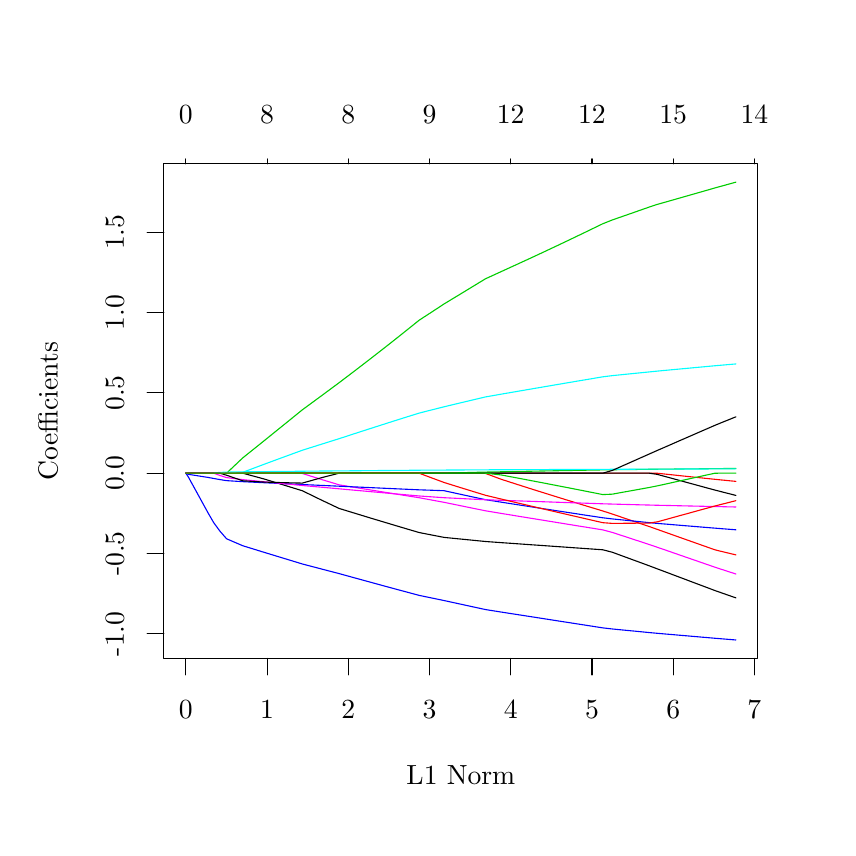
\begin{tikzpicture}[x=1pt,y=1pt]
\definecolor{fillColor}{RGB}{255,255,255}
\path[use as bounding box,fill=fillColor,fill opacity=0.00] (0,0) rectangle (289.08,289.08);
\begin{scope}
\path[clip] ( 49.20, 61.20) rectangle (263.88,239.88);
\definecolor{drawColor}{RGB}{0,0,0}

\path[draw=drawColor,line width= 0.4pt,line join=round,line cap=round] ( 57.15,128.09) --
	( 58.01,128.09) --
	( 60.63,128.09) --
	( 63.01,128.09) --
	( 65.19,128.09) --
	( 67.23,128.09) --
	( 69.45,128.09) --
	( 71.87,128.09) --
	( 77.71,128.09) --
	( 85.35,126.02) --
	( 92.54,123.81) --
	( 99.24,121.75) --
	(106.13,118.39) --
	(112.54,115.35) --
	(118.27,113.60) --
	(123.60,111.97) --
	(128.56,110.48) --
	(133.17,109.10) --
	(137.46,107.82) --
	(141.45,106.65) --
	(146.13,105.73) --
	(150.48,104.89) --
	(155.79,104.36) --
	(160.75,103.87) --
	(165.40,103.41) --
	(171.18,102.99) --
	(176.64,102.61) --
	(181.69,102.25) --
	(186.37,101.93) --
	(190.69,101.62) --
	(194.69,101.34) --
	(198.37,101.08) --
	(201.78,100.84) --
	(204.91,100.62) --
	(207.80,100.42) --
	(211.24, 99.53) --
	(215.01, 98.14) --
	(218.48, 96.87) --
	(221.67, 95.70) --
	(224.61, 94.62) --
	(227.46, 93.54) --
	(230.42, 92.44) --
	(233.18, 91.39) --
	(235.68, 90.45) --
	(237.97, 89.59) --
	(240.10, 88.78) --
	(242.02, 88.06) --
	(243.80, 87.39) --
	(245.41, 86.79) --
	(246.87, 86.24) --
	(248.23, 85.72) --
	(249.52, 85.27) --
	(250.72, 84.85) --
	(251.79, 84.48) --
	(252.74, 84.14) --
	(253.66, 83.82) --
	(254.50, 83.53) --
	(255.23, 83.27) --
	(255.93, 83.03);
\end{scope}
\begin{scope}
\path[clip] (  0.00,  0.00) rectangle (289.08,289.08);
\definecolor{drawColor}{RGB}{0,0,0}

\path[draw=drawColor,line width= 0.4pt,line join=round,line cap=round] ( 57.15, 61.20) -- (262.60, 61.20);

\path[draw=drawColor,line width= 0.4pt,line join=round,line cap=round] ( 57.15, 61.20) -- ( 57.15, 55.20);

\path[draw=drawColor,line width= 0.4pt,line join=round,line cap=round] ( 86.50, 61.20) -- ( 86.50, 55.20);

\path[draw=drawColor,line width= 0.4pt,line join=round,line cap=round] (115.85, 61.20) -- (115.85, 55.20);

\path[draw=drawColor,line width= 0.4pt,line join=round,line cap=round] (145.20, 61.20) -- (145.20, 55.20);

\path[draw=drawColor,line width= 0.4pt,line join=round,line cap=round] (174.55, 61.20) -- (174.55, 55.20);

\path[draw=drawColor,line width= 0.4pt,line join=round,line cap=round] (203.90, 61.20) -- (203.90, 55.20);

\path[draw=drawColor,line width= 0.4pt,line join=round,line cap=round] (233.25, 61.20) -- (233.25, 55.20);

\path[draw=drawColor,line width= 0.4pt,line join=round,line cap=round] (262.60, 61.20) -- (262.60, 55.20);

\node[text=drawColor,anchor=base,inner sep=0pt, outer sep=0pt, scale=  1.00] at ( 57.15, 39.60) {0};

\node[text=drawColor,anchor=base,inner sep=0pt, outer sep=0pt, scale=  1.00] at ( 86.50, 39.60) {1};

\node[text=drawColor,anchor=base,inner sep=0pt, outer sep=0pt, scale=  1.00] at (115.85, 39.60) {2};

\node[text=drawColor,anchor=base,inner sep=0pt, outer sep=0pt, scale=  1.00] at (145.20, 39.60) {3};

\node[text=drawColor,anchor=base,inner sep=0pt, outer sep=0pt, scale=  1.00] at (174.55, 39.60) {4};

\node[text=drawColor,anchor=base,inner sep=0pt, outer sep=0pt, scale=  1.00] at (203.90, 39.60) {5};

\node[text=drawColor,anchor=base,inner sep=0pt, outer sep=0pt, scale=  1.00] at (233.25, 39.60) {6};

\node[text=drawColor,anchor=base,inner sep=0pt, outer sep=0pt, scale=  1.00] at (262.60, 39.60) {7};

\path[draw=drawColor,line width= 0.4pt,line join=round,line cap=round] ( 49.20, 70.03) -- ( 49.20,215.18);

\path[draw=drawColor,line width= 0.4pt,line join=round,line cap=round] ( 49.20, 70.03) -- ( 43.20, 70.03);

\path[draw=drawColor,line width= 0.4pt,line join=round,line cap=round] ( 49.20, 99.06) -- ( 43.20, 99.06);

\path[draw=drawColor,line width= 0.4pt,line join=round,line cap=round] ( 49.20,128.09) -- ( 43.20,128.09);

\path[draw=drawColor,line width= 0.4pt,line join=round,line cap=round] ( 49.20,157.12) -- ( 43.20,157.12);

\path[draw=drawColor,line width= 0.4pt,line join=round,line cap=round] ( 49.20,186.15) -- ( 43.20,186.15);

\path[draw=drawColor,line width= 0.4pt,line join=round,line cap=round] ( 49.20,215.18) -- ( 43.20,215.18);

\node[text=drawColor,rotate= 90.00,anchor=base,inner sep=0pt, outer sep=0pt, scale=  1.00] at ( 34.80, 70.03) {-1.0};

\node[text=drawColor,rotate= 90.00,anchor=base,inner sep=0pt, outer sep=0pt, scale=  1.00] at ( 34.80, 99.06) {-0.5};

\node[text=drawColor,rotate= 90.00,anchor=base,inner sep=0pt, outer sep=0pt, scale=  1.00] at ( 34.80,128.09) {0.0};

\node[text=drawColor,rotate= 90.00,anchor=base,inner sep=0pt, outer sep=0pt, scale=  1.00] at ( 34.80,157.12) {0.5};

\node[text=drawColor,rotate= 90.00,anchor=base,inner sep=0pt, outer sep=0pt, scale=  1.00] at ( 34.80,186.15) {1.0};

\node[text=drawColor,rotate= 90.00,anchor=base,inner sep=0pt, outer sep=0pt, scale=  1.00] at ( 34.80,215.18) {1.5};

\path[draw=drawColor,line width= 0.4pt,line join=round,line cap=round] ( 49.20, 61.20) --
	(263.88, 61.20) --
	(263.88,239.88) --
	( 49.20,239.88) --
	( 49.20, 61.20);
\end{scope}
\begin{scope}
\path[clip] (  0.00,  0.00) rectangle (289.08,289.08);
\definecolor{drawColor}{RGB}{0,0,0}

\node[text=drawColor,anchor=base,inner sep=0pt, outer sep=0pt, scale=  1.00] at (156.54, 15.60) {L1 Norm};

\node[text=drawColor,rotate= 90.00,anchor=base,inner sep=0pt, outer sep=0pt, scale=  1.00] at ( 10.80,150.54) {Coefficients};
\end{scope}
\begin{scope}
\path[clip] ( 49.20, 61.20) rectangle (263.88,239.88);
\definecolor{drawColor}{RGB}{255,0,0}

\path[draw=drawColor,line width= 0.4pt,line join=round,line cap=round] ( 57.15,128.09) --
	( 58.01,128.09) --
	( 60.63,128.09) --
	( 63.01,128.09) --
	( 65.19,128.09) --
	( 67.23,128.09) --
	( 69.45,128.09) --
	( 71.87,128.09) --
	( 77.71,128.09) --
	( 85.35,128.09) --
	( 92.54,128.09) --
	( 99.24,128.09) --
	(106.13,128.09) --
	(112.54,128.09) --
	(118.27,128.09) --
	(123.60,128.09) --
	(128.56,128.09) --
	(133.17,128.09) --
	(137.46,128.09) --
	(141.45,128.09) --
	(146.13,128.09) --
	(150.48,128.09) --
	(155.79,128.09) --
	(160.75,128.09) --
	(165.40,128.09) --
	(171.18,128.09) --
	(176.64,128.09) --
	(181.69,128.09) --
	(186.37,128.09) --
	(190.69,128.09) --
	(194.69,128.09) --
	(198.37,128.09) --
	(201.78,128.09) --
	(204.91,128.09) --
	(207.80,128.09) --
	(211.24,128.09) --
	(215.01,128.09) --
	(218.48,128.09) --
	(221.67,128.09) --
	(224.61,128.09) --
	(227.46,128.08) --
	(230.42,127.76) --
	(233.18,127.47) --
	(235.68,127.20) --
	(237.97,126.96) --
	(240.10,126.74) --
	(242.02,126.53) --
	(243.80,126.35) --
	(245.41,126.18) --
	(246.87,126.03) --
	(248.23,125.89) --
	(249.52,125.76) --
	(250.72,125.64) --
	(251.79,125.54) --
	(252.74,125.44) --
	(253.66,125.35) --
	(254.50,125.27) --
	(255.23,125.20) --
	(255.93,125.13);
\definecolor{drawColor}{RGB}{0,205,0}

\path[draw=drawColor,line width= 0.4pt,line join=round,line cap=round] ( 57.15,128.09) --
	( 58.01,128.09) --
	( 60.63,128.09) --
	( 63.01,128.09) --
	( 65.19,128.09) --
	( 67.23,128.09) --
	( 69.45,128.09) --
	( 71.87,128.09) --
	( 77.71,133.61) --
	( 85.35,139.74) --
	( 92.54,145.55) --
	( 99.24,150.98) --
	(106.13,156.04) --
	(112.54,160.79) --
	(118.27,165.14) --
	(123.60,169.24) --
	(128.56,173.10) --
	(133.17,176.73) --
	(137.46,180.15) --
	(141.45,183.36) --
	(146.13,186.40) --
	(150.48,189.26) --
	(155.79,192.47) --
	(160.75,195.49) --
	(165.40,198.32) --
	(171.18,200.97) --
	(176.64,203.47) --
	(181.69,205.79) --
	(186.37,207.97) --
	(190.69,210.00) --
	(194.69,211.90) --
	(198.37,213.66) --
	(201.78,215.30) --
	(204.91,216.82) --
	(207.80,218.22) --
	(211.24,219.59) --
	(215.01,220.90) --
	(218.48,222.11) --
	(221.67,223.23) --
	(224.61,224.26) --
	(227.46,225.20) --
	(230.42,226.04) --
	(233.18,226.82) --
	(235.68,227.54) --
	(237.97,228.19) --
	(240.10,228.80) --
	(242.02,229.35) --
	(243.80,229.86) --
	(245.41,230.32) --
	(246.87,230.74) --
	(248.23,231.14) --
	(249.52,231.49) --
	(250.72,231.82) --
	(251.79,232.11) --
	(252.74,232.38) --
	(253.66,232.63) --
	(254.50,232.86) --
	(255.23,233.07) --
	(255.93,233.26);
\definecolor{drawColor}{RGB}{0,0,255}

\path[draw=drawColor,line width= 0.4pt,line join=round,line cap=round] ( 57.15,128.09) --
	( 58.01,126.80) --
	( 60.63,122.04) --
	( 63.01,117.70) --
	( 65.19,113.73) --
	( 67.23,110.20) --
	( 69.45,107.18) --
	( 71.87,104.39) --
	( 77.71,101.88) --
	( 85.35, 99.52) --
	( 92.54, 97.33) --
	( 99.24, 95.29) --
	(106.13, 93.48) --
	(112.54, 91.81) --
	(118.27, 90.23) --
	(123.60, 88.77) --
	(128.56, 87.41) --
	(133.17, 86.16) --
	(137.46, 85.01) --
	(141.45, 83.94) --
	(146.13, 82.97) --
	(150.48, 82.07) --
	(155.79, 80.91) --
	(160.75, 79.83) --
	(165.40, 78.82) --
	(171.18, 77.90) --
	(176.64, 77.05) --
	(181.69, 76.27) --
	(186.37, 75.54) --
	(190.69, 74.86) --
	(194.69, 74.24) --
	(198.37, 73.67) --
	(201.78, 73.14) --
	(204.91, 72.65) --
	(207.80, 72.20) --
	(211.24, 71.80) --
	(215.01, 71.43) --
	(218.48, 71.10) --
	(221.67, 70.79) --
	(224.61, 70.50) --
	(227.46, 70.24) --
	(230.42, 69.98) --
	(233.18, 69.75) --
	(235.68, 69.53) --
	(237.97, 69.34) --
	(240.10, 69.15) --
	(242.02, 68.99) --
	(243.80, 68.83) --
	(245.41, 68.70) --
	(246.87, 68.57) --
	(248.23, 68.45) --
	(249.52, 68.35) --
	(250.72, 68.25) --
	(251.79, 68.16) --
	(252.74, 68.08) --
	(253.66, 68.01) --
	(254.50, 67.94) --
	(255.23, 67.88) --
	(255.93, 67.82);
\definecolor{drawColor}{RGB}{0,255,255}

\path[draw=drawColor,line width= 0.4pt,line join=round,line cap=round] ( 57.15,128.09) --
	( 58.01,128.09) --
	( 60.63,128.09) --
	( 63.01,128.09) --
	( 65.19,128.09) --
	( 67.23,128.09) --
	( 69.45,128.09) --
	( 71.87,128.09) --
	( 77.71,128.41) --
	( 85.35,131.28) --
	( 92.54,133.93) --
	( 99.24,136.38) --
	(106.13,138.55) --
	(112.54,140.56) --
	(118.27,142.43) --
	(123.60,144.15) --
	(128.56,145.74) --
	(133.17,147.21) --
	(137.46,148.56) --
	(141.45,149.80) --
	(146.13,150.99) --
	(150.48,152.09) --
	(155.79,153.36) --
	(160.75,154.54) --
	(165.40,155.64) --
	(171.18,156.66) --
	(176.64,157.60) --
	(181.69,158.47) --
	(186.37,159.27) --
	(190.69,160.01) --
	(194.69,160.69) --
	(198.37,161.32) --
	(201.78,161.89) --
	(204.91,162.42) --
	(207.80,162.91) --
	(211.24,163.34) --
	(215.01,163.72) --
	(218.48,164.07) --
	(221.67,164.39) --
	(224.61,164.68) --
	(227.46,164.97) --
	(230.42,165.25) --
	(233.18,165.51) --
	(235.68,165.74) --
	(237.97,165.95) --
	(240.10,166.15) --
	(242.02,166.33) --
	(243.80,166.49) --
	(245.41,166.64) --
	(246.87,166.78) --
	(248.23,166.90) --
	(249.52,167.02) --
	(250.72,167.12) --
	(251.79,167.21) --
	(252.74,167.30) --
	(253.66,167.38) --
	(254.50,167.45) --
	(255.23,167.51) --
	(255.93,167.57);
\definecolor{drawColor}{RGB}{255,0,255}

\path[draw=drawColor,line width= 0.4pt,line join=round,line cap=round] ( 57.15,128.09) --
	( 58.01,128.09) --
	( 60.63,128.09) --
	( 63.01,128.09) --
	( 65.19,128.09) --
	( 67.23,128.09) --
	( 69.45,128.09) --
	( 71.87,128.09) --
	( 77.71,128.09) --
	( 85.35,128.09) --
	( 92.54,128.09) --
	( 99.24,128.00) --
	(106.13,125.83) --
	(112.54,123.88) --
	(118.27,122.94) --
	(123.60,122.08) --
	(128.56,121.28) --
	(133.17,120.54) --
	(137.46,119.86) --
	(141.45,119.23) --
	(146.13,118.36) --
	(150.48,117.56) --
	(155.79,116.47) --
	(160.75,115.45) --
	(165.40,114.51) --
	(171.18,113.55) --
	(176.64,112.65) --
	(181.69,111.83) --
	(186.37,111.07) --
	(190.69,110.37) --
	(194.69,109.72) --
	(198.37,109.12) --
	(201.78,108.58) --
	(204.91,108.07) --
	(207.80,107.61) --
	(211.24,106.69) --
	(215.01,105.46) --
	(218.48,104.32) --
	(221.67,103.28) --
	(224.61,102.32) --
	(227.46,101.34) --
	(230.42,100.33) --
	(233.18, 99.37) --
	(235.68, 98.50) --
	(237.97, 97.71) --
	(240.10, 96.97) --
	(242.02, 96.31) --
	(243.80, 95.69) --
	(245.41, 95.13) --
	(246.87, 94.63) --
	(248.23, 94.15) --
	(249.52, 93.73) --
	(250.72, 93.34) --
	(251.79, 93.00) --
	(252.74, 92.69) --
	(253.66, 92.39) --
	(254.50, 92.12) --
	(255.23, 91.88) --
	(255.93, 91.65);
\definecolor{drawColor}{RGB}{0,0,0}

\path[draw=drawColor,line width= 0.4pt,line join=round,line cap=round] ( 57.15,128.09) --
	( 58.01,128.09) --
	( 60.63,128.09) --
	( 63.01,128.09) --
	( 65.19,128.09) --
	( 67.23,128.09) --
	( 69.45,128.09) --
	( 71.87,128.09) --
	( 77.71,128.09) --
	( 85.35,128.09) --
	( 92.54,128.09) --
	( 99.24,128.09) --
	(106.13,128.09) --
	(112.54,128.09) --
	(118.27,128.09) --
	(123.60,128.09) --
	(128.56,128.09) --
	(133.17,128.09) --
	(137.46,128.09) --
	(141.45,128.09) --
	(146.13,128.09) --
	(150.48,128.09) --
	(155.79,128.09) --
	(160.75,128.09) --
	(165.40,128.09) --
	(171.18,128.09) --
	(176.64,128.09) --
	(181.69,128.09) --
	(186.37,128.09) --
	(190.69,128.09) --
	(194.69,128.09) --
	(198.37,128.09) --
	(201.78,128.09) --
	(204.91,128.09) --
	(207.80,128.09) --
	(211.24,128.09) --
	(215.01,128.09) --
	(218.48,128.09) --
	(221.67,128.09) --
	(224.61,128.09) --
	(227.46,127.67) --
	(230.42,126.87) --
	(233.18,126.12) --
	(235.68,125.44) --
	(237.97,124.81) --
	(240.10,124.23) --
	(242.02,123.71) --
	(243.80,123.22) --
	(245.41,122.78) --
	(246.87,122.39) --
	(248.23,122.02) --
	(249.52,121.69) --
	(250.72,121.38) --
	(251.79,121.11) --
	(252.74,120.87) --
	(253.66,120.63) --
	(254.50,120.42) --
	(255.23,120.23) --
	(255.93,120.05);
\definecolor{drawColor}{RGB}{255,0,0}

\path[draw=drawColor,line width= 0.4pt,line join=round,line cap=round] ( 57.15,128.09) --
	( 58.01,128.09) --
	( 60.63,128.09) --
	( 63.01,128.09) --
	( 65.19,128.09) --
	( 67.23,128.09) --
	( 69.45,128.09) --
	( 71.87,128.09) --
	( 77.71,128.09) --
	( 85.35,128.09) --
	( 92.54,128.09) --
	( 99.24,128.09) --
	(106.13,128.09) --
	(112.54,128.09) --
	(118.27,128.09) --
	(123.60,128.09) --
	(128.56,128.09) --
	(133.17,128.09) --
	(137.46,128.09) --
	(141.45,128.09) --
	(146.13,128.09) --
	(150.48,128.09) --
	(155.79,128.09) --
	(160.75,128.09) --
	(165.40,128.02) --
	(171.18,125.87) --
	(176.64,124.11) --
	(181.69,122.50) --
	(186.37,121.03) --
	(190.69,119.68) --
	(194.69,118.44) --
	(198.37,117.31) --
	(201.78,116.27) --
	(204.91,115.32) --
	(207.80,114.45) --
	(211.24,113.33) --
	(215.01,112.05) --
	(218.48,110.88) --
	(221.67,109.80) --
	(224.61,108.81) --
	(227.46,107.80) --
	(230.42,106.75) --
	(233.18,105.77) --
	(235.68,104.88) --
	(237.97,104.07) --
	(240.10,103.32) --
	(242.02,102.64) --
	(243.80,102.00) --
	(245.41,101.44) --
	(246.87,100.92) --
	(248.23,100.44) --
	(249.52,100.10) --
	(250.72, 99.82) --
	(251.79, 99.56) --
	(252.74, 99.33) --
	(253.66, 99.11) --
	(254.50, 98.91) --
	(255.23, 98.73) --
	(255.93, 98.57);
\definecolor{drawColor}{RGB}{0,205,0}

\path[draw=drawColor,line width= 0.4pt,line join=round,line cap=round] ( 57.15,128.09) --
	( 58.01,128.09) --
	( 60.63,128.09) --
	( 63.01,128.09) --
	( 65.19,128.09) --
	( 67.23,128.09) --
	( 69.45,128.09) --
	( 71.87,128.09) --
	( 77.71,128.09) --
	( 85.35,128.09) --
	( 92.54,128.09) --
	( 99.24,128.09) --
	(106.13,128.09) --
	(112.54,128.09) --
	(118.27,128.09) --
	(123.60,128.09) --
	(128.56,128.09) --
	(133.17,128.09) --
	(137.46,128.09) --
	(141.45,128.09) --
	(146.13,128.09) --
	(150.48,128.10) --
	(155.79,128.24) --
	(160.75,128.37) --
	(165.40,128.49) --
	(171.18,128.60) --
	(176.64,128.71) --
	(181.69,128.80) --
	(186.37,128.89) --
	(190.69,128.97) --
	(194.69,129.04) --
	(198.37,129.11) --
	(201.78,129.17) --
	(204.91,129.23) --
	(207.80,129.28) --
	(211.24,129.33) --
	(215.01,129.38) --
	(218.48,129.42) --
	(221.67,129.46) --
	(224.61,129.50) --
	(227.46,129.53) --
	(230.42,129.56) --
	(233.18,129.58) --
	(235.68,129.61) --
	(237.97,129.63) --
	(240.10,129.65) --
	(242.02,129.67) --
	(243.80,129.69) --
	(245.41,129.71) --
	(246.87,129.72) --
	(248.23,129.73) --
	(249.52,129.75) --
	(250.72,129.76) --
	(251.79,129.77) --
	(252.74,129.78) --
	(253.66,129.78) --
	(254.50,129.79) --
	(255.23,129.80) --
	(255.93,129.81);
\definecolor{drawColor}{RGB}{0,0,255}

\path[draw=drawColor,line width= 0.4pt,line join=round,line cap=round] ( 57.15,128.09) --
	( 58.01,127.69) --
	( 60.63,127.28) --
	( 63.01,126.90) --
	( 65.19,126.56) --
	( 67.23,126.18) --
	( 69.45,125.78) --
	( 71.87,125.40) --
	( 77.71,125.03) --
	( 85.35,124.65) --
	( 92.54,124.31) --
	( 99.24,123.99) --
	(106.13,123.68) --
	(112.54,123.39) --
	(118.27,123.13) --
	(123.60,122.89) --
	(128.56,122.66) --
	(133.17,122.45) --
	(137.46,122.26) --
	(141.45,122.08) --
	(146.13,121.92) --
	(150.48,121.76) --
	(155.79,120.60) --
	(160.75,119.52) --
	(165.40,118.53) --
	(171.18,117.61) --
	(176.64,116.76) --
	(181.69,115.98) --
	(186.37,115.25) --
	(190.69,114.59) --
	(194.69,113.98) --
	(198.37,113.42) --
	(201.78,112.89) --
	(204.91,112.42) --
	(207.80,111.98) --
	(211.24,111.57) --
	(215.01,111.19) --
	(218.48,110.84) --
	(221.67,110.52) --
	(224.61,110.22) --
	(227.46,109.95) --
	(230.42,109.71) --
	(233.18,109.48) --
	(235.68,109.27) --
	(237.97,109.08) --
	(240.10,108.91) --
	(242.02,108.75) --
	(243.80,108.60) --
	(245.41,108.47) --
	(246.87,108.35) --
	(248.23,108.24) --
	(249.52,108.14) --
	(250.72,108.04) --
	(251.79,107.96) --
	(252.74,107.88) --
	(253.66,107.81) --
	(254.50,107.75) --
	(255.23,107.69) --
	(255.93,107.63);
\definecolor{drawColor}{RGB}{0,255,255}

\path[draw=drawColor,line width= 0.4pt,line join=round,line cap=round] ( 57.15,128.09) --
	( 58.01,128.09) --
	( 60.63,128.09) --
	( 63.01,128.09) --
	( 65.19,128.09) --
	( 67.23,128.22) --
	( 69.45,128.36) --
	( 71.87,128.48) --
	( 77.71,128.58) --
	( 85.35,128.66) --
	( 92.54,128.73) --
	( 99.24,128.80) --
	(106.13,128.87) --
	(112.54,128.92) --
	(118.27,128.97) --
	(123.60,129.02) --
	(128.56,129.06) --
	(133.17,129.10) --
	(137.46,129.13) --
	(141.45,129.17) --
	(146.13,129.19) --
	(150.48,129.22) --
	(155.79,129.25) --
	(160.75,129.28) --
	(165.40,129.31) --
	(171.18,129.33) --
	(176.64,129.36) --
	(181.69,129.38) --
	(186.37,129.40) --
	(190.69,129.41) --
	(194.69,129.43) --
	(198.37,129.45) --
	(201.78,129.46) --
	(204.91,129.47) --
	(207.80,129.48) --
	(211.24,129.50) --
	(215.01,129.51) --
	(218.48,129.53) --
	(221.67,129.54) --
	(224.61,129.55) --
	(227.46,129.57) --
	(230.42,129.57) --
	(233.18,129.58) --
	(235.68,129.59) --
	(237.97,129.60) --
	(240.10,129.60) --
	(242.02,129.61) --
	(243.80,129.62) --
	(245.41,129.62) --
	(246.87,129.63) --
	(248.23,129.63) --
	(249.52,129.63) --
	(250.72,129.64) --
	(251.79,129.64) --
	(252.74,129.64) --
	(253.66,129.65) --
	(254.50,129.65) --
	(255.23,129.65) --
	(255.93,129.65);
\definecolor{drawColor}{RGB}{255,0,255}

\path[draw=drawColor,line width= 0.4pt,line join=round,line cap=round] ( 57.15,128.09) --
	( 58.01,128.09) --
	( 60.63,128.09) --
	( 63.01,128.09) --
	( 65.19,128.09) --
	( 67.23,128.08) --
	( 69.45,127.27) --
	( 71.87,126.50) --
	( 77.71,125.76) --
	( 85.35,125.01) --
	( 92.54,124.30) --
	( 99.24,123.64) --
	(106.13,123.03) --
	(112.54,122.45) --
	(118.27,121.93) --
	(123.60,121.45) --
	(128.56,121.01) --
	(133.17,120.59) --
	(137.46,120.21) --
	(141.45,119.86) --
	(146.13,119.53) --
	(150.48,119.23) --
	(155.79,118.97) --
	(160.75,118.72) --
	(165.40,118.49) --
	(171.18,118.29) --
	(176.64,118.10) --
	(181.69,117.93) --
	(186.37,117.77) --
	(190.69,117.62) --
	(194.69,117.48) --
	(198.37,117.35) --
	(201.78,117.24) --
	(204.91,117.13) --
	(207.80,117.03) --
	(211.24,116.93) --
	(215.01,116.83) --
	(218.48,116.74) --
	(221.67,116.65) --
	(224.61,116.58) --
	(227.46,116.50) --
	(230.42,116.44) --
	(233.18,116.38) --
	(235.68,116.32) --
	(237.97,116.27) --
	(240.10,116.22) --
	(242.02,116.18) --
	(243.80,116.14) --
	(245.41,116.10) --
	(246.87,116.07) --
	(248.23,116.04) --
	(249.52,116.01) --
	(250.72,115.99) --
	(251.79,115.97) --
	(252.74,115.94) --
	(253.66,115.93) --
	(254.50,115.91) --
	(255.23,115.89) --
	(255.93,115.88);
\definecolor{drawColor}{RGB}{0,0,0}

\path[draw=drawColor,line width= 0.4pt,line join=round,line cap=round] ( 57.15,128.09) --
	( 58.01,128.09) --
	( 60.63,128.09) --
	( 63.01,128.09) --
	( 65.19,128.09) --
	( 67.23,128.09) --
	( 69.45,128.09) --
	( 71.87,127.35) --
	( 77.71,125.35) --
	( 85.35,124.88) --
	( 92.54,124.66) --
	( 99.24,124.51) --
	(106.13,126.45) --
	(112.54,128.09) --
	(118.27,128.09) --
	(123.60,128.09) --
	(128.56,128.09) --
	(133.17,128.09) --
	(137.46,128.09) --
	(141.45,128.09) --
	(146.13,128.09) --
	(150.48,128.09) --
	(155.79,128.09) --
	(160.75,128.09) --
	(165.40,128.09) --
	(171.18,128.09) --
	(176.64,128.09) --
	(181.69,128.09) --
	(186.37,128.09) --
	(190.69,128.09) --
	(194.69,128.09) --
	(198.37,128.09) --
	(201.78,128.09) --
	(204.91,128.09) --
	(207.80,128.09) --
	(211.24,129.08) --
	(215.01,130.76) --
	(218.48,132.30) --
	(221.67,133.72) --
	(224.61,135.02) --
	(227.46,136.29) --
	(230.42,137.57) --
	(233.18,138.78) --
	(235.68,139.88) --
	(237.97,140.87) --
	(240.10,141.80) --
	(242.02,142.64) --
	(243.80,143.42) --
	(245.41,144.11) --
	(246.87,144.75) --
	(248.23,145.34) --
	(249.52,145.87) --
	(250.72,146.36) --
	(251.79,146.79) --
	(252.74,147.17) --
	(253.66,147.54) --
	(254.50,147.89) --
	(255.23,148.18) --
	(255.93,148.46);
\definecolor{drawColor}{RGB}{255,0,0}

\path[draw=drawColor,line width= 0.4pt,line join=round,line cap=round] ( 57.15,128.09) --
	( 58.01,128.09) --
	( 60.63,128.09) --
	( 63.01,128.09) --
	( 65.19,128.09) --
	( 67.23,128.09) --
	( 69.45,128.09) --
	( 71.87,128.09) --
	( 77.71,128.09) --
	( 85.35,128.09) --
	( 92.54,128.09) --
	( 99.24,128.09) --
	(106.13,128.09) --
	(112.54,128.09) --
	(118.27,128.09) --
	(123.60,128.09) --
	(128.56,128.09) --
	(133.17,128.09) --
	(137.46,128.09) --
	(141.45,128.09) --
	(146.13,126.34) --
	(150.48,124.73) --
	(155.79,123.07) --
	(160.75,121.54) --
	(165.40,120.12) --
	(171.18,118.73) --
	(176.64,117.44) --
	(181.69,116.25) --
	(186.37,115.16) --
	(190.69,114.15) --
	(194.69,113.23) --
	(198.37,112.38) --
	(201.78,111.59) --
	(204.91,110.87) --
	(207.80,110.21) --
	(211.24,109.95) --
	(215.01,109.98) --
	(218.48,110.01) --
	(221.67,110.04) --
	(224.61,110.07) --
	(227.46,110.50) --
	(230.42,111.30) --
	(233.18,112.07) --
	(235.68,112.76) --
	(237.97,113.38) --
	(240.10,113.97) --
	(242.02,114.50) --
	(243.80,114.99) --
	(245.41,115.43) --
	(246.87,115.83) --
	(248.23,116.21) --
	(249.52,116.54) --
	(250.72,116.85) --
	(251.79,117.11) --
	(252.74,117.35) --
	(253.66,117.58) --
	(254.50,117.80) --
	(255.23,117.98) --
	(255.93,118.16);
\definecolor{drawColor}{RGB}{0,205,0}

\path[draw=drawColor,line width= 0.4pt,line join=round,line cap=round] ( 57.15,128.09) --
	( 58.01,128.09) --
	( 60.63,128.09) --
	( 63.01,128.09) --
	( 65.19,128.09) --
	( 67.23,128.09) --
	( 69.45,128.09) --
	( 71.87,128.09) --
	( 77.71,128.09) --
	( 85.35,128.09) --
	( 92.54,128.09) --
	( 99.24,128.09) --
	(106.13,128.09) --
	(112.54,128.09) --
	(118.27,128.09) --
	(123.60,128.09) --
	(128.56,128.09) --
	(133.17,128.09) --
	(137.46,128.09) --
	(141.45,128.09) --
	(146.13,128.09) --
	(150.48,128.09) --
	(155.79,128.09) --
	(160.75,128.09) --
	(165.40,128.09) --
	(171.18,127.44) --
	(176.64,126.41) --
	(181.69,125.45) --
	(186.37,124.56) --
	(190.69,123.72) --
	(194.69,122.95) --
	(198.37,122.23) --
	(201.78,121.56) --
	(204.91,120.94) --
	(207.80,120.36) --
	(211.24,120.51) --
	(215.01,121.20) --
	(218.48,121.82) --
	(221.67,122.40) --
	(224.61,122.93) --
	(227.46,123.50) --
	(230.42,124.14) --
	(233.18,124.76) --
	(235.68,125.31) --
	(237.97,125.81) --
	(240.10,126.28) --
	(242.02,126.70) --
	(243.80,127.10) --
	(245.41,127.45) --
	(246.87,127.76) --
	(248.23,128.06) --
	(249.52,128.09) --
	(250.72,128.09) --
	(251.79,128.09) --
	(252.74,128.09) --
	(253.66,128.09) --
	(254.50,128.09) --
	(255.23,128.09) --
	(255.93,128.09);
\end{scope}
\begin{scope}
\path[clip] (  0.00,  0.00) rectangle (289.08,289.08);
\definecolor{drawColor}{RGB}{0,0,0}

\path[draw=drawColor,line width= 0.4pt,line join=round,line cap=round] ( 57.15,239.88) -- (262.60,239.88);

\path[draw=drawColor,line width= 0.4pt,line join=round,line cap=round] ( 57.15,239.88) -- ( 57.15,241.67);

\path[draw=drawColor,line width= 0.4pt,line join=round,line cap=round] ( 86.50,239.88) -- ( 86.50,241.67);

\path[draw=drawColor,line width= 0.4pt,line join=round,line cap=round] (115.85,239.88) -- (115.85,241.67);

\path[draw=drawColor,line width= 0.4pt,line join=round,line cap=round] (145.20,239.88) -- (145.20,241.67);

\path[draw=drawColor,line width= 0.4pt,line join=round,line cap=round] (174.55,239.88) -- (174.55,241.67);

\path[draw=drawColor,line width= 0.4pt,line join=round,line cap=round] (203.90,239.88) -- (203.90,241.67);

\path[draw=drawColor,line width= 0.4pt,line join=round,line cap=round] (233.25,239.88) -- (233.25,241.67);

\path[draw=drawColor,line width= 0.4pt,line join=round,line cap=round] (262.60,239.88) -- (262.60,241.67);

\node[text=drawColor,anchor=base,inner sep=0pt, outer sep=0pt, scale=  1.00] at ( 57.15,254.28) {0};

\node[text=drawColor,anchor=base,inner sep=0pt, outer sep=0pt, scale=  1.00] at ( 86.50,254.28) {8};

\node[text=drawColor,anchor=base,inner sep=0pt, outer sep=0pt, scale=  1.00] at (115.85,254.28) {8};

\node[text=drawColor,anchor=base,inner sep=0pt, outer sep=0pt, scale=  1.00] at (145.20,254.28) {9};

\node[text=drawColor,anchor=base,inner sep=0pt, outer sep=0pt, scale=  1.00] at (174.55,254.28) {12};

\node[text=drawColor,anchor=base,inner sep=0pt, outer sep=0pt, scale=  1.00] at (203.90,254.28) {12};

\node[text=drawColor,anchor=base,inner sep=0pt, outer sep=0pt, scale=  1.00] at (233.25,254.28) {15};

\node[text=drawColor,anchor=base,inner sep=0pt, outer sep=0pt, scale=  1.00] at (262.60,254.28) {14};
\end{scope}
\end{tikzpicture}
}
	\caption{Regularization path of the Lasso. Lines with different colours correspond to different covariates.} \label{lassopath}
    \end{subfigure}%
    \begin{subfigure}[t]{.5\textwidth} \centering
	\resizebox{\textwidth}{!}{%
	    % Created by tikzDevice version 0.11 on 2018-04-28 11:50:00
% !TEX encoding = UTF-8 Unicode
\begin{tikzpicture}[x=1pt,y=1pt]
\definecolor{fillColor}{RGB}{255,255,255}
\path[use as bounding box,fill=fillColor,fill opacity=0.00] (0,0) rectangle (289.08,289.08);
\begin{scope}
\path[clip] (  0.00,  0.00) rectangle (289.08,289.08);
\definecolor{drawColor}{RGB}{0,0,0}

\path[draw=drawColor,line width= 0.4pt,line join=round,line cap=round] ( 49.71, 61.20) -- (110.95, 61.20);

\path[draw=drawColor,line width= 0.4pt,line join=round,line cap=round] ( 49.71, 61.20) -- ( 49.71, 55.20);

\path[draw=drawColor,line width= 0.4pt,line join=round,line cap=round] ( 61.96, 61.20) -- ( 61.96, 55.20);

\path[draw=drawColor,line width= 0.4pt,line join=round,line cap=round] ( 74.21, 61.20) -- ( 74.21, 55.20);

\path[draw=drawColor,line width= 0.4pt,line join=round,line cap=round] ( 86.45, 61.20) -- ( 86.45, 55.20);

\path[draw=drawColor,line width= 0.4pt,line join=round,line cap=round] ( 98.70, 61.20) -- ( 98.70, 55.20);

\path[draw=drawColor,line width= 0.4pt,line join=round,line cap=round] (110.95, 61.20) -- (110.95, 55.20);

\node[text=drawColor,anchor=base,inner sep=0pt, outer sep=0pt, scale=  1.00] at ( 49.71, 39.60) {-8};

\node[text=drawColor,anchor=base,inner sep=0pt, outer sep=0pt, scale=  1.00] at ( 74.21, 39.60) {-6};

\node[text=drawColor,anchor=base,inner sep=0pt, outer sep=0pt, scale=  1.00] at ( 98.70, 39.60) {-4};

\path[draw=drawColor,line width= 0.4pt,line join=round,line cap=round] ( 49.20, 85.92) -- ( 49.20,197.88);

\path[draw=drawColor,line width= 0.4pt,line join=round,line cap=round] ( 49.20, 85.92) -- ( 43.20, 85.92);

\path[draw=drawColor,line width= 0.4pt,line join=round,line cap=round] ( 49.20,141.90) -- ( 43.20,141.90);

\path[draw=drawColor,line width= 0.4pt,line join=round,line cap=round] ( 49.20,197.88) -- ( 43.20,197.88);

\node[text=drawColor,rotate= 90.00,anchor=base,inner sep=0pt, outer sep=0pt, scale=  1.00] at ( 34.80, 85.92) {1.25};

\node[text=drawColor,rotate= 90.00,anchor=base,inner sep=0pt, outer sep=0pt, scale=  1.00] at ( 34.80,141.90) {1.30};

\node[text=drawColor,rotate= 90.00,anchor=base,inner sep=0pt, outer sep=0pt, scale=  1.00] at ( 34.80,197.88) {1.35};

\path[draw=drawColor,line width= 0.4pt,line join=round,line cap=round] ( 49.20, 61.20) --
	(119.34, 61.20) --
	(119.34,239.88) --
	( 49.20,239.88) --
	( 49.20, 61.20);
\end{scope}
\begin{scope}
\path[clip] (  0.00,  0.00) rectangle (144.54,289.08);
\definecolor{drawColor}{RGB}{0,0,0}

\node[text=drawColor,anchor=base,inner sep=0pt, outer sep=0pt, scale=  1.00] at ( 84.27, 15.60) {log(Lambda)};

\node[text=drawColor,rotate= 90.00,anchor=base,inner sep=0pt, outer sep=0pt, scale=  1.00] at ( 10.80,150.54) {Binomial Deviance};
\end{scope}
\begin{scope}
\path[clip] ( 49.20, 61.20) rectangle (119.34,239.88);
\definecolor{drawColor}{RGB}{169,169,169}

\path[draw=drawColor,line width= 0.4pt,line join=round,line cap=round] (116.74,233.26) -- (116.74,229.06);

\path[draw=drawColor,line width= 0.4pt,line join=round,line cap=round] (115.60,226.74) -- (115.60,223.35);

\path[draw=drawColor,line width= 0.4pt,line join=round,line cap=round] (114.46,218.56) -- (114.46,214.50);

\path[draw=drawColor,line width= 0.4pt,line join=round,line cap=round] (113.32,210.99) -- (113.32,206.41);

\path[draw=drawColor,line width= 0.4pt,line join=round,line cap=round] (112.18,204.56) -- (112.18,199.49);

\path[draw=drawColor,line width= 0.4pt,line join=round,line cap=round] (111.05,196.33) -- (111.05,190.84);

\path[draw=drawColor,line width= 0.4pt,line join=round,line cap=round] (109.91,187.74) -- (109.91,181.46);

\path[draw=drawColor,line width= 0.4pt,line join=round,line cap=round] (108.77,179.23) -- (108.77,172.31);

\path[draw=drawColor,line width= 0.4pt,line join=round,line cap=round] (107.63,170.42) -- (107.63,163.03);

\path[draw=drawColor,line width= 0.4pt,line join=round,line cap=round] (106.49,161.26) -- (106.49,153.59);

\path[draw=drawColor,line width= 0.4pt,line join=round,line cap=round] (105.35,153.23) -- (105.35,145.19);

\path[draw=drawColor,line width= 0.4pt,line join=round,line cap=round] (104.21,146.20) -- (104.21,137.38);

\path[draw=drawColor,line width= 0.4pt,line join=round,line cap=round] (103.07,140.14) -- (103.07,130.57);

\path[draw=drawColor,line width= 0.4pt,line join=round,line cap=round] (101.93,135.04) -- (101.93,124.83);

\path[draw=drawColor,line width= 0.4pt,line join=round,line cap=round] (100.79,130.58) -- (100.79,120.02);

\path[draw=drawColor,line width= 0.4pt,line join=round,line cap=round] ( 99.65,126.68) -- ( 99.65,115.98);

\path[draw=drawColor,line width= 0.4pt,line join=round,line cap=round] ( 98.51,123.47) -- ( 98.51,112.56);

\path[draw=drawColor,line width= 0.4pt,line join=round,line cap=round] ( 97.37,120.85) -- ( 97.37,109.67);

\path[draw=drawColor,line width= 0.4pt,line join=round,line cap=round] ( 96.23,118.65) -- ( 96.23,107.21);

\path[draw=drawColor,line width= 0.4pt,line join=round,line cap=round] ( 95.09,116.80) -- ( 95.09,105.11);

\path[draw=drawColor,line width= 0.4pt,line join=round,line cap=round] ( 93.95,115.25) -- ( 93.95,103.31);

\path[draw=drawColor,line width= 0.4pt,line join=round,line cap=round] ( 92.82,113.31) -- ( 92.82,100.96);

\path[draw=drawColor,line width= 0.4pt,line join=round,line cap=round] ( 91.68,109.47) -- ( 91.68, 97.29);

\path[draw=drawColor,line width= 0.4pt,line join=round,line cap=round] ( 90.54,105.19) -- ( 90.54, 92.92);

\path[draw=drawColor,line width= 0.4pt,line join=round,line cap=round] ( 89.40,101.53) -- ( 89.40, 89.13);

\path[draw=drawColor,line width= 0.4pt,line join=round,line cap=round] ( 88.26, 98.47) -- ( 88.26, 85.92);

\path[draw=drawColor,line width= 0.4pt,line join=round,line cap=round] ( 87.12, 95.92) -- ( 87.12, 83.18);

\path[draw=drawColor,line width= 0.4pt,line join=round,line cap=round] ( 85.98, 93.80) -- ( 85.98, 80.85);

\path[draw=drawColor,line width= 0.4pt,line join=round,line cap=round] ( 84.84, 92.05) -- ( 84.84, 78.88);

\path[draw=drawColor,line width= 0.4pt,line join=round,line cap=round] ( 83.70, 90.60) -- ( 83.70, 77.23);

\path[draw=drawColor,line width= 0.4pt,line join=round,line cap=round] ( 82.56, 89.40) -- ( 82.56, 75.83);

\path[draw=drawColor,line width= 0.4pt,line join=round,line cap=round] ( 81.42, 88.42) -- ( 81.42, 74.64);

\path[draw=drawColor,line width= 0.4pt,line join=round,line cap=round] ( 80.28, 87.62) -- ( 80.28, 73.64);

\path[draw=drawColor,line width= 0.4pt,line join=round,line cap=round] ( 79.14, 86.97) -- ( 79.14, 72.80);

\path[draw=drawColor,line width= 0.4pt,line join=round,line cap=round] ( 78.00, 86.43) -- ( 78.00, 72.04);

\path[draw=drawColor,line width= 0.4pt,line join=round,line cap=round] ( 76.86, 85.91) -- ( 76.86, 71.34);

\path[draw=drawColor,line width= 0.4pt,line join=round,line cap=round] ( 75.72, 85.46) -- ( 75.72, 70.70);

\path[draw=drawColor,line width= 0.4pt,line join=round,line cap=round] ( 74.59, 85.10) -- ( 74.59, 70.17);

\path[draw=drawColor,line width= 0.4pt,line join=round,line cap=round] ( 73.45, 84.71) -- ( 73.45, 69.71);

\path[draw=drawColor,line width= 0.4pt,line join=round,line cap=round] ( 72.31, 84.38) -- ( 72.31, 69.32);

\path[draw=drawColor,line width= 0.4pt,line join=round,line cap=round] ( 71.17, 84.11) -- ( 71.17, 69.00);

\path[draw=drawColor,line width= 0.4pt,line join=round,line cap=round] ( 70.03, 83.90) -- ( 70.03, 68.74);

\path[draw=drawColor,line width= 0.4pt,line join=round,line cap=round] ( 68.89, 83.74) -- ( 68.89, 68.53);

\path[draw=drawColor,line width= 0.4pt,line join=round,line cap=round] ( 67.75, 83.60) -- ( 67.75, 68.35);

\path[draw=drawColor,line width= 0.4pt,line join=round,line cap=round] ( 66.61, 83.50) -- ( 66.61, 68.21);

\path[draw=drawColor,line width= 0.4pt,line join=round,line cap=round] ( 65.47, 83.41) -- ( 65.47, 68.09);

\path[draw=drawColor,line width= 0.4pt,line join=round,line cap=round] ( 64.33, 83.35) -- ( 64.33, 68.01);

\path[draw=drawColor,line width= 0.4pt,line join=round,line cap=round] ( 63.19, 83.31) -- ( 63.19, 67.95);

\path[draw=drawColor,line width= 0.4pt,line join=round,line cap=round] ( 62.05, 83.28) -- ( 62.05, 67.91);

\path[draw=drawColor,line width= 0.4pt,line join=round,line cap=round] ( 60.91, 83.26) -- ( 60.91, 67.88);

\path[draw=drawColor,line width= 0.4pt,line join=round,line cap=round] ( 59.77, 83.25) -- ( 59.77, 67.86);

\path[draw=drawColor,line width= 0.4pt,line join=round,line cap=round] ( 58.63, 83.25) -- ( 58.63, 67.84);

\path[draw=drawColor,line width= 0.4pt,line join=round,line cap=round] ( 57.49, 83.25) -- ( 57.49, 67.83);

\path[draw=drawColor,line width= 0.4pt,line join=round,line cap=round] ( 56.36, 83.25) -- ( 56.36, 67.83);

\path[draw=drawColor,line width= 0.4pt,line join=round,line cap=round] ( 55.22, 83.26) -- ( 55.22, 67.82);

\path[draw=drawColor,line width= 0.4pt,line join=round,line cap=round] ( 54.08, 83.26) -- ( 54.08, 67.82);

\path[draw=drawColor,line width= 0.4pt,line join=round,line cap=round] ( 52.94, 83.27) -- ( 52.94, 67.82);

\path[draw=drawColor,line width= 0.4pt,line join=round,line cap=round] ( 51.80, 83.27) -- ( 51.80, 67.82);

\path[draw=drawColor,line width= 0.4pt,line join=round,line cap=round] (116.09,233.26) -- (117.39,233.26);

\path[draw=drawColor,line width= 0.4pt,line join=round,line cap=round] (114.95,226.74) -- (116.25,226.74);

\path[draw=drawColor,line width= 0.4pt,line join=round,line cap=round] (113.81,218.56) -- (115.11,218.56);

\path[draw=drawColor,line width= 0.4pt,line join=round,line cap=round] (112.67,210.99) -- (113.97,210.99);

\path[draw=drawColor,line width= 0.4pt,line join=round,line cap=round] (111.54,204.56) -- (112.83,204.56);

\path[draw=drawColor,line width= 0.4pt,line join=round,line cap=round] (110.40,196.33) -- (111.69,196.33);

\path[draw=drawColor,line width= 0.4pt,line join=round,line cap=round] (109.26,187.74) -- (110.56,187.74);

\path[draw=drawColor,line width= 0.4pt,line join=round,line cap=round] (108.12,179.23) -- (109.42,179.23);

\path[draw=drawColor,line width= 0.4pt,line join=round,line cap=round] (106.98,170.42) -- (108.28,170.42);

\path[draw=drawColor,line width= 0.4pt,line join=round,line cap=round] (105.84,161.26) -- (107.14,161.26);

\path[draw=drawColor,line width= 0.4pt,line join=round,line cap=round] (104.70,153.23) -- (106.00,153.23);

\path[draw=drawColor,line width= 0.4pt,line join=round,line cap=round] (103.56,146.20) -- (104.86,146.20);

\path[draw=drawColor,line width= 0.4pt,line join=round,line cap=round] (102.42,140.14) -- (103.72,140.14);

\path[draw=drawColor,line width= 0.4pt,line join=round,line cap=round] (101.28,135.04) -- (102.58,135.04);

\path[draw=drawColor,line width= 0.4pt,line join=round,line cap=round] (100.14,130.58) -- (101.44,130.58);

\path[draw=drawColor,line width= 0.4pt,line join=round,line cap=round] ( 99.00,126.68) -- (100.30,126.68);

\path[draw=drawColor,line width= 0.4pt,line join=round,line cap=round] ( 97.86,123.47) -- ( 99.16,123.47);

\path[draw=drawColor,line width= 0.4pt,line join=round,line cap=round] ( 96.72,120.85) -- ( 98.02,120.85);

\path[draw=drawColor,line width= 0.4pt,line join=round,line cap=round] ( 95.58,118.65) -- ( 96.88,118.65);

\path[draw=drawColor,line width= 0.4pt,line join=round,line cap=round] ( 94.44,116.80) -- ( 95.74,116.80);

\path[draw=drawColor,line width= 0.4pt,line join=round,line cap=round] ( 93.31,115.25) -- ( 94.60,115.25);

\path[draw=drawColor,line width= 0.4pt,line join=round,line cap=round] ( 92.17,113.31) -- ( 93.46,113.31);

\path[draw=drawColor,line width= 0.4pt,line join=round,line cap=round] ( 91.03,109.47) -- ( 92.33,109.47);

\path[draw=drawColor,line width= 0.4pt,line join=round,line cap=round] ( 89.89,105.19) -- ( 91.19,105.19);

\path[draw=drawColor,line width= 0.4pt,line join=round,line cap=round] ( 88.75,101.53) -- ( 90.05,101.53);

\path[draw=drawColor,line width= 0.4pt,line join=round,line cap=round] ( 87.61, 98.47) -- ( 88.91, 98.47);

\path[draw=drawColor,line width= 0.4pt,line join=round,line cap=round] ( 86.47, 95.92) -- ( 87.77, 95.92);

\path[draw=drawColor,line width= 0.4pt,line join=round,line cap=round] ( 85.33, 93.80) -- ( 86.63, 93.80);

\path[draw=drawColor,line width= 0.4pt,line join=round,line cap=round] ( 84.19, 92.05) -- ( 85.49, 92.05);

\path[draw=drawColor,line width= 0.4pt,line join=round,line cap=round] ( 83.05, 90.60) -- ( 84.35, 90.60);

\path[draw=drawColor,line width= 0.4pt,line join=round,line cap=round] ( 81.91, 89.40) -- ( 83.21, 89.40);

\path[draw=drawColor,line width= 0.4pt,line join=round,line cap=round] ( 80.77, 88.42) -- ( 82.07, 88.42);

\path[draw=drawColor,line width= 0.4pt,line join=round,line cap=round] ( 79.63, 87.62) -- ( 80.93, 87.62);

\path[draw=drawColor,line width= 0.4pt,line join=round,line cap=round] ( 78.49, 86.97) -- ( 79.79, 86.97);

\path[draw=drawColor,line width= 0.4pt,line join=round,line cap=round] ( 77.35, 86.43) -- ( 78.65, 86.43);

\path[draw=drawColor,line width= 0.4pt,line join=round,line cap=round] ( 76.21, 85.91) -- ( 77.51, 85.91);

\path[draw=drawColor,line width= 0.4pt,line join=round,line cap=round] ( 75.08, 85.46) -- ( 76.37, 85.46);

\path[draw=drawColor,line width= 0.4pt,line join=round,line cap=round] ( 73.94, 85.10) -- ( 75.23, 85.10);

\path[draw=drawColor,line width= 0.4pt,line join=round,line cap=round] ( 72.80, 84.71) -- ( 74.10, 84.71);

\path[draw=drawColor,line width= 0.4pt,line join=round,line cap=round] ( 71.66, 84.38) -- ( 72.96, 84.38);

\path[draw=drawColor,line width= 0.4pt,line join=round,line cap=round] ( 70.52, 84.11) -- ( 71.82, 84.11);

\path[draw=drawColor,line width= 0.4pt,line join=round,line cap=round] ( 69.38, 83.90) -- ( 70.68, 83.90);

\path[draw=drawColor,line width= 0.4pt,line join=round,line cap=round] ( 68.24, 83.74) -- ( 69.54, 83.74);

\path[draw=drawColor,line width= 0.4pt,line join=round,line cap=round] ( 67.10, 83.60) -- ( 68.40, 83.60);

\path[draw=drawColor,line width= 0.4pt,line join=round,line cap=round] ( 65.96, 83.50) -- ( 67.26, 83.50);

\path[draw=drawColor,line width= 0.4pt,line join=round,line cap=round] ( 64.82, 83.41) -- ( 66.12, 83.41);

\path[draw=drawColor,line width= 0.4pt,line join=round,line cap=round] ( 63.68, 83.35) -- ( 64.98, 83.35);

\path[draw=drawColor,line width= 0.4pt,line join=round,line cap=round] ( 62.54, 83.31) -- ( 63.84, 83.31);

\path[draw=drawColor,line width= 0.4pt,line join=round,line cap=round] ( 61.40, 83.28) -- ( 62.70, 83.28);

\path[draw=drawColor,line width= 0.4pt,line join=round,line cap=round] ( 60.26, 83.26) -- ( 61.56, 83.26);

\path[draw=drawColor,line width= 0.4pt,line join=round,line cap=round] ( 59.12, 83.25) -- ( 60.42, 83.25);

\path[draw=drawColor,line width= 0.4pt,line join=round,line cap=round] ( 57.98, 83.25) -- ( 59.28, 83.25);

\path[draw=drawColor,line width= 0.4pt,line join=round,line cap=round] ( 56.85, 83.25) -- ( 58.14, 83.25);

\path[draw=drawColor,line width= 0.4pt,line join=round,line cap=round] ( 55.71, 83.25) -- ( 57.00, 83.25);

\path[draw=drawColor,line width= 0.4pt,line join=round,line cap=round] ( 54.57, 83.26) -- ( 55.87, 83.26);

\path[draw=drawColor,line width= 0.4pt,line join=round,line cap=round] ( 53.43, 83.26) -- ( 54.73, 83.26);

\path[draw=drawColor,line width= 0.4pt,line join=round,line cap=round] ( 52.29, 83.27) -- ( 53.59, 83.27);

\path[draw=drawColor,line width= 0.4pt,line join=round,line cap=round] ( 51.15, 83.27) -- ( 52.45, 83.27);

\path[draw=drawColor,line width= 0.4pt,line join=round,line cap=round] (116.09,229.06) -- (117.39,229.06);

\path[draw=drawColor,line width= 0.4pt,line join=round,line cap=round] (114.95,223.35) -- (116.25,223.35);

\path[draw=drawColor,line width= 0.4pt,line join=round,line cap=round] (113.81,214.50) -- (115.11,214.50);

\path[draw=drawColor,line width= 0.4pt,line join=round,line cap=round] (112.67,206.41) -- (113.97,206.41);

\path[draw=drawColor,line width= 0.4pt,line join=round,line cap=round] (111.54,199.49) -- (112.83,199.49);

\path[draw=drawColor,line width= 0.4pt,line join=round,line cap=round] (110.40,190.84) -- (111.69,190.84);

\path[draw=drawColor,line width= 0.4pt,line join=round,line cap=round] (109.26,181.46) -- (110.56,181.46);

\path[draw=drawColor,line width= 0.4pt,line join=round,line cap=round] (108.12,172.31) -- (109.42,172.31);

\path[draw=drawColor,line width= 0.4pt,line join=round,line cap=round] (106.98,163.03) -- (108.28,163.03);

\path[draw=drawColor,line width= 0.4pt,line join=round,line cap=round] (105.84,153.59) -- (107.14,153.59);

\path[draw=drawColor,line width= 0.4pt,line join=round,line cap=round] (104.70,145.19) -- (106.00,145.19);

\path[draw=drawColor,line width= 0.4pt,line join=round,line cap=round] (103.56,137.38) -- (104.86,137.38);

\path[draw=drawColor,line width= 0.4pt,line join=round,line cap=round] (102.42,130.57) -- (103.72,130.57);

\path[draw=drawColor,line width= 0.4pt,line join=round,line cap=round] (101.28,124.83) -- (102.58,124.83);

\path[draw=drawColor,line width= 0.4pt,line join=round,line cap=round] (100.14,120.02) -- (101.44,120.02);

\path[draw=drawColor,line width= 0.4pt,line join=round,line cap=round] ( 99.00,115.98) -- (100.30,115.98);

\path[draw=drawColor,line width= 0.4pt,line join=round,line cap=round] ( 97.86,112.56) -- ( 99.16,112.56);

\path[draw=drawColor,line width= 0.4pt,line join=round,line cap=round] ( 96.72,109.67) -- ( 98.02,109.67);

\path[draw=drawColor,line width= 0.4pt,line join=round,line cap=round] ( 95.58,107.21) -- ( 96.88,107.21);

\path[draw=drawColor,line width= 0.4pt,line join=round,line cap=round] ( 94.44,105.11) -- ( 95.74,105.11);

\path[draw=drawColor,line width= 0.4pt,line join=round,line cap=round] ( 93.31,103.31) -- ( 94.60,103.31);

\path[draw=drawColor,line width= 0.4pt,line join=round,line cap=round] ( 92.17,100.96) -- ( 93.46,100.96);

\path[draw=drawColor,line width= 0.4pt,line join=round,line cap=round] ( 91.03, 97.29) -- ( 92.33, 97.29);

\path[draw=drawColor,line width= 0.4pt,line join=round,line cap=round] ( 89.89, 92.92) -- ( 91.19, 92.92);

\path[draw=drawColor,line width= 0.4pt,line join=round,line cap=round] ( 88.75, 89.13) -- ( 90.05, 89.13);

\path[draw=drawColor,line width= 0.4pt,line join=round,line cap=round] ( 87.61, 85.92) -- ( 88.91, 85.92);

\path[draw=drawColor,line width= 0.4pt,line join=round,line cap=round] ( 86.47, 83.18) -- ( 87.77, 83.18);

\path[draw=drawColor,line width= 0.4pt,line join=round,line cap=round] ( 85.33, 80.85) -- ( 86.63, 80.85);

\path[draw=drawColor,line width= 0.4pt,line join=round,line cap=round] ( 84.19, 78.88) -- ( 85.49, 78.88);

\path[draw=drawColor,line width= 0.4pt,line join=round,line cap=round] ( 83.05, 77.23) -- ( 84.35, 77.23);

\path[draw=drawColor,line width= 0.4pt,line join=round,line cap=round] ( 81.91, 75.83) -- ( 83.21, 75.83);

\path[draw=drawColor,line width= 0.4pt,line join=round,line cap=round] ( 80.77, 74.64) -- ( 82.07, 74.64);

\path[draw=drawColor,line width= 0.4pt,line join=round,line cap=round] ( 79.63, 73.64) -- ( 80.93, 73.64);

\path[draw=drawColor,line width= 0.4pt,line join=round,line cap=round] ( 78.49, 72.80) -- ( 79.79, 72.80);

\path[draw=drawColor,line width= 0.4pt,line join=round,line cap=round] ( 77.35, 72.04) -- ( 78.65, 72.04);

\path[draw=drawColor,line width= 0.4pt,line join=round,line cap=round] ( 76.21, 71.34) -- ( 77.51, 71.34);

\path[draw=drawColor,line width= 0.4pt,line join=round,line cap=round] ( 75.08, 70.70) -- ( 76.37, 70.70);

\path[draw=drawColor,line width= 0.4pt,line join=round,line cap=round] ( 73.94, 70.17) -- ( 75.23, 70.17);

\path[draw=drawColor,line width= 0.4pt,line join=round,line cap=round] ( 72.80, 69.71) -- ( 74.10, 69.71);

\path[draw=drawColor,line width= 0.4pt,line join=round,line cap=round] ( 71.66, 69.32) -- ( 72.96, 69.32);

\path[draw=drawColor,line width= 0.4pt,line join=round,line cap=round] ( 70.52, 69.00) -- ( 71.82, 69.00);

\path[draw=drawColor,line width= 0.4pt,line join=round,line cap=round] ( 69.38, 68.74) -- ( 70.68, 68.74);

\path[draw=drawColor,line width= 0.4pt,line join=round,line cap=round] ( 68.24, 68.53) -- ( 69.54, 68.53);

\path[draw=drawColor,line width= 0.4pt,line join=round,line cap=round] ( 67.10, 68.35) -- ( 68.40, 68.35);

\path[draw=drawColor,line width= 0.4pt,line join=round,line cap=round] ( 65.96, 68.21) -- ( 67.26, 68.21);

\path[draw=drawColor,line width= 0.4pt,line join=round,line cap=round] ( 64.82, 68.09) -- ( 66.12, 68.09);

\path[draw=drawColor,line width= 0.4pt,line join=round,line cap=round] ( 63.68, 68.01) -- ( 64.98, 68.01);

\path[draw=drawColor,line width= 0.4pt,line join=round,line cap=round] ( 62.54, 67.95) -- ( 63.84, 67.95);

\path[draw=drawColor,line width= 0.4pt,line join=round,line cap=round] ( 61.40, 67.91) -- ( 62.70, 67.91);

\path[draw=drawColor,line width= 0.4pt,line join=round,line cap=round] ( 60.26, 67.88) -- ( 61.56, 67.88);

\path[draw=drawColor,line width= 0.4pt,line join=round,line cap=round] ( 59.12, 67.86) -- ( 60.42, 67.86);

\path[draw=drawColor,line width= 0.4pt,line join=round,line cap=round] ( 57.98, 67.84) -- ( 59.28, 67.84);

\path[draw=drawColor,line width= 0.4pt,line join=round,line cap=round] ( 56.85, 67.83) -- ( 58.14, 67.83);

\path[draw=drawColor,line width= 0.4pt,line join=round,line cap=round] ( 55.71, 67.83) -- ( 57.00, 67.83);

\path[draw=drawColor,line width= 0.4pt,line join=round,line cap=round] ( 54.57, 67.82) -- ( 55.87, 67.82);

\path[draw=drawColor,line width= 0.4pt,line join=round,line cap=round] ( 53.43, 67.82) -- ( 54.73, 67.82);

\path[draw=drawColor,line width= 0.4pt,line join=round,line cap=round] ( 52.29, 67.82) -- ( 53.59, 67.82);

\path[draw=drawColor,line width= 0.4pt,line join=round,line cap=round] ( 51.15, 67.82) -- ( 52.45, 67.82);
\definecolor{drawColor}{RGB}{255,0,0}
\definecolor{fillColor}{RGB}{255,0,0}

\path[draw=drawColor,line width= 0.4pt,line join=round,line cap=round,fill=fillColor] (116.74,231.16) circle (  1.50);

\path[draw=drawColor,line width= 0.4pt,line join=round,line cap=round,fill=fillColor] (115.60,225.05) circle (  1.50);

\path[draw=drawColor,line width= 0.4pt,line join=round,line cap=round,fill=fillColor] (114.46,216.53) circle (  1.50);

\path[draw=drawColor,line width= 0.4pt,line join=round,line cap=round,fill=fillColor] (113.32,208.70) circle (  1.50);

\path[draw=drawColor,line width= 0.4pt,line join=round,line cap=round,fill=fillColor] (112.18,202.03) circle (  1.50);

\path[draw=drawColor,line width= 0.4pt,line join=round,line cap=round,fill=fillColor] (111.05,193.58) circle (  1.50);

\path[draw=drawColor,line width= 0.4pt,line join=round,line cap=round,fill=fillColor] (109.91,184.60) circle (  1.50);

\path[draw=drawColor,line width= 0.4pt,line join=round,line cap=round,fill=fillColor] (108.77,175.77) circle (  1.50);

\path[draw=drawColor,line width= 0.4pt,line join=round,line cap=round,fill=fillColor] (107.63,166.73) circle (  1.50);

\path[draw=drawColor,line width= 0.4pt,line join=round,line cap=round,fill=fillColor] (106.49,157.42) circle (  1.50);

\path[draw=drawColor,line width= 0.4pt,line join=round,line cap=round,fill=fillColor] (105.35,149.21) circle (  1.50);

\path[draw=drawColor,line width= 0.4pt,line join=round,line cap=round,fill=fillColor] (104.21,141.79) circle (  1.50);

\path[draw=drawColor,line width= 0.4pt,line join=round,line cap=round,fill=fillColor] (103.07,135.35) circle (  1.50);

\path[draw=drawColor,line width= 0.4pt,line join=round,line cap=round,fill=fillColor] (101.93,129.94) circle (  1.50);

\path[draw=drawColor,line width= 0.4pt,line join=round,line cap=round,fill=fillColor] (100.79,125.30) circle (  1.50);

\path[draw=drawColor,line width= 0.4pt,line join=round,line cap=round,fill=fillColor] ( 99.65,121.33) circle (  1.50);

\path[draw=drawColor,line width= 0.4pt,line join=round,line cap=round,fill=fillColor] ( 98.51,118.01) circle (  1.50);

\path[draw=drawColor,line width= 0.4pt,line join=round,line cap=round,fill=fillColor] ( 97.37,115.26) circle (  1.50);

\path[draw=drawColor,line width= 0.4pt,line join=round,line cap=round,fill=fillColor] ( 96.23,112.93) circle (  1.50);

\path[draw=drawColor,line width= 0.4pt,line join=round,line cap=round,fill=fillColor] ( 95.09,110.96) circle (  1.50);

\path[draw=drawColor,line width= 0.4pt,line join=round,line cap=round,fill=fillColor] ( 93.95,109.28) circle (  1.50);

\path[draw=drawColor,line width= 0.4pt,line join=round,line cap=round,fill=fillColor] ( 92.82,107.13) circle (  1.50);

\path[draw=drawColor,line width= 0.4pt,line join=round,line cap=round,fill=fillColor] ( 91.68,103.38) circle (  1.50);

\path[draw=drawColor,line width= 0.4pt,line join=round,line cap=round,fill=fillColor] ( 90.54, 99.05) circle (  1.50);

\path[draw=drawColor,line width= 0.4pt,line join=round,line cap=round,fill=fillColor] ( 89.40, 95.33) circle (  1.50);

\path[draw=drawColor,line width= 0.4pt,line join=round,line cap=round,fill=fillColor] ( 88.26, 92.19) circle (  1.50);

\path[draw=drawColor,line width= 0.4pt,line join=round,line cap=round,fill=fillColor] ( 87.12, 89.55) circle (  1.50);

\path[draw=drawColor,line width= 0.4pt,line join=round,line cap=round,fill=fillColor] ( 85.98, 87.33) circle (  1.50);

\path[draw=drawColor,line width= 0.4pt,line join=round,line cap=round,fill=fillColor] ( 84.84, 85.47) circle (  1.50);

\path[draw=drawColor,line width= 0.4pt,line join=round,line cap=round,fill=fillColor] ( 83.70, 83.91) circle (  1.50);

\path[draw=drawColor,line width= 0.4pt,line join=round,line cap=round,fill=fillColor] ( 82.56, 82.62) circle (  1.50);

\path[draw=drawColor,line width= 0.4pt,line join=round,line cap=round,fill=fillColor] ( 81.42, 81.53) circle (  1.50);

\path[draw=drawColor,line width= 0.4pt,line join=round,line cap=round,fill=fillColor] ( 80.28, 80.63) circle (  1.50);

\path[draw=drawColor,line width= 0.4pt,line join=round,line cap=round,fill=fillColor] ( 79.14, 79.88) circle (  1.50);

\path[draw=drawColor,line width= 0.4pt,line join=round,line cap=round,fill=fillColor] ( 78.00, 79.23) circle (  1.50);

\path[draw=drawColor,line width= 0.4pt,line join=round,line cap=round,fill=fillColor] ( 76.86, 78.63) circle (  1.50);

\path[draw=drawColor,line width= 0.4pt,line join=round,line cap=round,fill=fillColor] ( 75.72, 78.08) circle (  1.50);

\path[draw=drawColor,line width= 0.4pt,line join=round,line cap=round,fill=fillColor] ( 74.59, 77.63) circle (  1.50);

\path[draw=drawColor,line width= 0.4pt,line join=round,line cap=round,fill=fillColor] ( 73.45, 77.21) circle (  1.50);

\path[draw=drawColor,line width= 0.4pt,line join=round,line cap=round,fill=fillColor] ( 72.31, 76.85) circle (  1.50);

\path[draw=drawColor,line width= 0.4pt,line join=round,line cap=round,fill=fillColor] ( 71.17, 76.56) circle (  1.50);

\path[draw=drawColor,line width= 0.4pt,line join=round,line cap=round,fill=fillColor] ( 70.03, 76.32) circle (  1.50);

\path[draw=drawColor,line width= 0.4pt,line join=round,line cap=round,fill=fillColor] ( 68.89, 76.13) circle (  1.50);

\path[draw=drawColor,line width= 0.4pt,line join=round,line cap=round,fill=fillColor] ( 67.75, 75.98) circle (  1.50);

\path[draw=drawColor,line width= 0.4pt,line join=round,line cap=round,fill=fillColor] ( 66.61, 75.85) circle (  1.50);

\path[draw=drawColor,line width= 0.4pt,line join=round,line cap=round,fill=fillColor] ( 65.47, 75.75) circle (  1.50);

\path[draw=drawColor,line width= 0.4pt,line join=round,line cap=round,fill=fillColor] ( 64.33, 75.68) circle (  1.50);

\path[draw=drawColor,line width= 0.4pt,line join=round,line cap=round,fill=fillColor] ( 63.19, 75.63) circle (  1.50);

\path[draw=drawColor,line width= 0.4pt,line join=round,line cap=round,fill=fillColor] ( 62.05, 75.59) circle (  1.50);

\path[draw=drawColor,line width= 0.4pt,line join=round,line cap=round,fill=fillColor] ( 60.91, 75.57) circle (  1.50);

\path[draw=drawColor,line width= 0.4pt,line join=round,line cap=round,fill=fillColor] ( 59.77, 75.56) circle (  1.50);

\path[draw=drawColor,line width= 0.4pt,line join=round,line cap=round,fill=fillColor] ( 58.63, 75.55) circle (  1.50);

\path[draw=drawColor,line width= 0.4pt,line join=round,line cap=round,fill=fillColor] ( 57.49, 75.54) circle (  1.50);

\path[draw=drawColor,line width= 0.4pt,line join=round,line cap=round,fill=fillColor] ( 56.36, 75.54) circle (  1.50);

\path[draw=drawColor,line width= 0.4pt,line join=round,line cap=round,fill=fillColor] ( 55.22, 75.54) circle (  1.50);

\path[draw=drawColor,line width= 0.4pt,line join=round,line cap=round,fill=fillColor] ( 54.08, 75.54) circle (  1.50);

\path[draw=drawColor,line width= 0.4pt,line join=round,line cap=round,fill=fillColor] ( 52.94, 75.54) circle (  1.50);

\path[draw=drawColor,line width= 0.4pt,line join=round,line cap=round,fill=fillColor] ( 51.80, 75.55) circle (  1.50);
\end{scope}
\begin{scope}
\path[clip] (  0.00,  0.00) rectangle (289.08,289.08);
\definecolor{drawColor}{RGB}{0,0,0}

\node[text=drawColor,anchor=base,inner sep=0pt, outer sep=0pt, scale=  1.00] at ( 51.80,254.28) {14};

\node[text=drawColor,anchor=base,inner sep=0pt, outer sep=0pt, scale=  1.00] at ( 71.17,254.28) {15};

\node[text=drawColor,anchor=base,inner sep=0pt, outer sep=0pt, scale=  1.00] at ( 90.54,254.28) {10};

\node[text=drawColor,anchor=base,inner sep=0pt, outer sep=0pt, scale=  1.00] at (106.49,254.28) {8};
\end{scope}
\begin{scope}
\path[clip] ( 49.20, 61.20) rectangle (119.34,239.88);
\definecolor{drawColor}{RGB}{0,0,0}

\path[draw=drawColor,line width= 0.4pt,dash pattern=on 1pt off 3pt ,line join=round,line cap=round] ( 54.08, 61.20) -- ( 54.08,239.88);

\path[draw=drawColor,line width= 0.4pt,dash pattern=on 1pt off 3pt ,line join=round,line cap=round] ( 82.56, 61.20) -- ( 82.56,239.88);
\end{scope}
\end{tikzpicture}
}
	\caption{Binomial deviance against regularization parameter by 5-fold CV.} \label{lassocv}
    \end{subfigure}
    \caption{Results of the GAM.}
\end{figure}

\par The AIC of the lasso model is not given automatically by package \texttt{glmnet}. Nonetheless, the computation is tractable theoretically, as the effective degrees of freedom are shown to be the expectation of trace of active-set data matrix \cite{tibshirani:2012:dflasso}. For now, we will resort to AUC as an alternative assessment method. AUC for 5-fold cross validated lasso is 0.7118, smaller than that of ordinary logistic regression, which may indicate a lack of information (dimension) to tackle the problem.

\subsection{Generalized Additive Model}
Apart from the methods described above, we can adapt more flexible techniques in the modeling of covariates, since logit transformation has been done on the response variable. In a regression setting, GAM has the form
\begin{align}
\log\left(\frac{p}{1-p}\right)=\alpha+f_1(x_1)+f_2(x_2)+\dots+f_p(x_p)
\end{align}
for a model of $p$ predictors. Here, we define $f_i$'s as any unspecified functions whose forms are yet to be decided either parametrically or nonparametrially. 
\par Basis expansion is one of the possibilities of data augmentation for capturing non-linear relationship between the predictors and transformed response. A \noun{Natural Cubic Spline} (NCS) \cite{Friedman:2001:ESL} with $K$ nodes ($\tau_1<\tau_2<\dots<\tau_K$) can be represented by, in total, $K$ parametric basis functions.
\begin{align}
f_1(x)=1,\quad f_2(x)=x, \quad \ldots, \quad f_{k+2}(x)=d_k(x)-d_{K-1}(x)
\end{align}
where
\begin{align}
d_{k}=\frac{(x-\tau_k)^3_+-(x-\tau_K)^3_+}{\tau_K-\tau_k},\quad k=1,\dots,K.
\end{align}
NCS is, in fact, ordinary cubic splines with additional constraints on boundary nodes, which assert linearity beyond the range of observed data. This assumption is valid in that cubic splines usually inflate drastically around the boundaries, as little information is available in that region. Categorical variables cannot be modeled by splines and are left as ordinary predictors. The model fitted by integrating NCS (with 3 knots) with GLM gives AIC=5493.7. Under 5\% level of significance, all predictors should be retained in the model, including the interaction effect of \texttt{degree} and \texttt{status}, as suggested previously.
\par Other than parametric modeling, there have been several nonparametric statistical tools which aim at delineating the relationship between the dependent and independent variables in a more flexible manner. One of the most famous techniques is the \noun{Locally Weighted Scatterplot Smoothing} (LOESS) regression \cite{Friedman:2001:ESL}. It takes data points in a neighborhood $\mathcal{N}(x)$ centered at current $x$ and use weighed least square to minimize
\begin{align}
\sum_{i, x_i\in \mathcal{N}(x)}\left[\log\left(\frac{p_i}{1-p_i}\right)-\beta_0-\beta_1(x_i-x)\right]^2W\left(\frac{|x-x_i|}{\delta_x}\right)
\end{align}
for fixed $x$, where $\delta_x=\underset{x_i\in \mathcal{N}(x)}{\max}|x-x_i|$ denotes the diameter of the neighborhood. Then, estimation of fitted values is carried out by traversing the whole linear space. AUC of loess regression (with \texttt{span=0.2}) embedded in the context of GAM is 5570.2. Altering the levels of \texttt{span} does not change much the resulted AIC.
\par We now compute the AUC of the model fitted with NCS, which has a smaller AIC, as 0.7286, which is superior to logistic regression. However, interpretability is hurt for predictors expanded by NCS. Hence, we will only elaborate a few preliminary but interesting findings from the logistic regression. 

\par Here, we omit insignificant levels of categorical predictors for easier analysis. The acceptance rate for \texttt{PhD} application is significantly lower than that for \texttt{MS}. Results released through \texttt{Phone} are more likely to be an offer rather than a rejection letter, followed by \texttt{Email} and \texttt{Website}. This makes sense because important and urgent decisions are often transmitted though more efficient and effective communication tools. U.S. students have a bigger chance to get admitted, compared to students from other backgrounds. While this might be the case, it is worth noticing that,
counterintuitively, international students who apply for \texttt{PhD} degrees has the best shot of admission
(noted the magnitude of the interaction term).
This is not inline with the general perception and experience. One possible explanation is that the dataset
may be not very representative in that the many international applicants may be not very familiar with
\noun{GradCafe}, and may not be willing to post an entry if the applicant is not successful. Hence,
we cautiously leave the test for this hypothesis for future work when more representative data are available.
Candidates who has higher \texttt{gpa} and \texttt{gre} scores are preferred. Moreover, it is more difficult to secure a place in universities with higher rankings, as anticipated, and those with more faculty members tend to take in more applicants.
\begin{table}
\centering
\begin{tabular}{l|ccc}
\hline
Effect & Estimate & Std. Error & \textit{p}-value \\
\hline
    \texttt{decision\_methodPhone} &  1.846362 & 0.319259 & $7.33\times 10^{-9}$ \\
\texttt{degreePhD:statusInternational} & 0.405409 & 0.162446 & 0.0126 \\
\hline
\end{tabular}
\caption{Some coefficients fitted with logistic regression.}
\end{table}


\section{Tree-Based Ensemble Learners} \label{sec: tree}
In this section, we explored the tree-based ensemble learners. 
\subsection{Random Forests} \label{sub: rf}
The essential idea in bagging is to average many noisy but approximately unbiased models, since trees is of instability due to its the hierarchical nature. However, if each tree generated in bagging is identically distributed but not necessarily independent, the correlation of the pairs of bagged trees would limit the benefits of averaging. Random Forest decorrelate the trees via split-variable randomization. Besides, Random Forest does not increase the variance too much, which is achieved through the random selection of split predictors \cite{Friedman:2001:ESL}.\\ 
For \textbf{GradCafe} dataset, natural splines of the numeric predictors significantly improve the performance of Random Forests, according to the metric, AUC. 
\begin{table}[h]
    \centering
    \begin{tabular}{|c|c|c|}
      \hline 
    Parameter & Value & Explanation \\ 
    \hline 
        \var{mtry} & 9 & Randomly Selected Predictors\\
    \hline 
        \var{splitrule} & extratrees & Splitting Rule \\
        \hline 
        \var{min.node.size} & 6 & Minimum size of terminal nodes \\
    \hline 
    \end{tabular}
    \caption{The value of tuning parameters used in Random Forests}
    \label{tab:rf}
\end{table}
By 5-fold cross validation with the metric AUC, the value of tuning parameters are chosen as shown in the Table \ref{tab:rf}. \\
Figure \ref{fig: xgb} displays the variable importance for each of the predictor variables. \var{uni\_pub}, \var{decision\_month}, and \var{uni\_faculty} are predominantly relevant with the result of application. \var{GRE} and \var{GPA} have roughly half relevance of \var{uni\_pub}, whereas others do not show strong relevance. The AUC of training set is 0.8361. 
\begin{figure}[htb]
    \centering
    \begin{subfigure}{.5\linewidth}
	\centering
	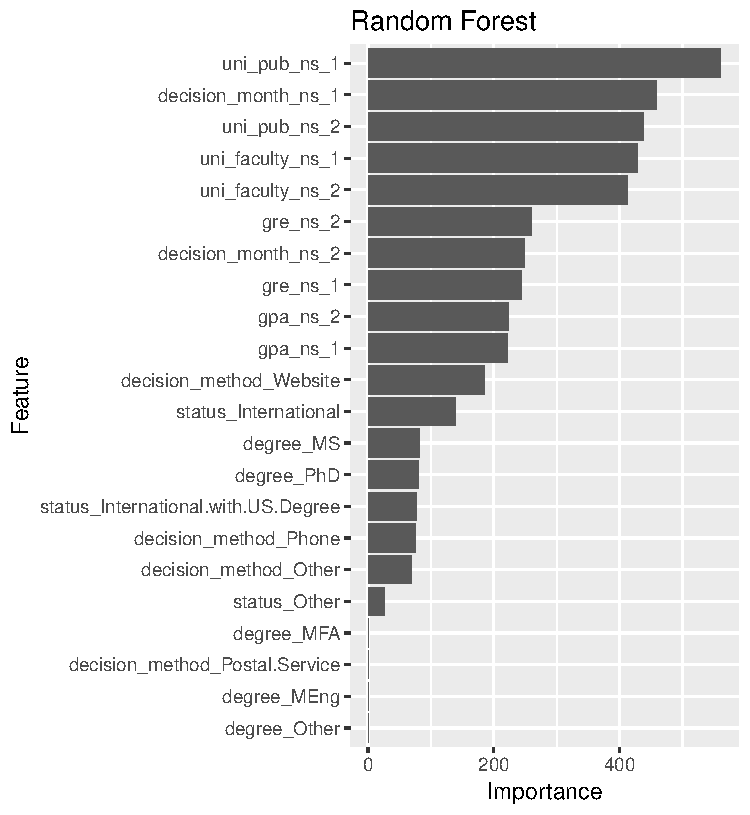
\includegraphics[width = \linewidth]{RF.pdf}
	\caption{Variable importace plots for the classification random forest grown on the \textbf{GradCafe} data.}
	\label{fig:rf}
    \end{subfigure}%
    \begin{subfigure}{.5\linewidth}
    \centering
    \includegraphics[width = \linewidth]{xgboost.pdf}
    \caption{The predictor variable importance in descending order for \textbf{GradCafe} dataset using XGBoost.}
    \label{fig: xgb}
\end{subfigure}
    \caption{Feature selection for \noun{GradCafe} ensemble learner.}
\end{figure}
The AUC of random forest on test data is 0.7558307. 

\subsection{eXtreame Gradient Boosting} \label{sub: xgb}
XGBoost is a scalable end-to-end tree boosting system, which uses far fewer resources than existing systems in billions of examples. The key problem in tree learning is to find the best split, and XGBoost uses the exact greedy algorithm. The novel tree learning algorithm of XGBoost algorithm is proposed for handling sparse data, and a theoretically justified weighted quantile sketch for approximate tree learning proposes candidate split points. The sparsity-aware split finding speeds up the computation time. Besides, the tuning parameter $Column Subsampling$ is borrowed from Random Forest. \\
Time complexity $O(Kd\left\|\mathbf{x}\right\|_0+\left\|\mathbf{x}\right\|_0\log B)$, where $d$ is the maximum depth of the tree, $K$ is the total number of trees, $B$ is the maximum number of rows in each block and $\left\|\mathbf{x}\right\|_0$ denotes the number of non-missing entries in the training data \cite{chen:2016:xgboost}. \\
The design matrix is made by using R library, {\itshape recipe} in the similar as mentioned before. R library, {\itshape xgboost}, is used for fitting XGBoost. \\
After evaluating the variable importance, we selected following interaction terms, including interactions between $status$ and $uni\_pub$, $gpa$ and $gre$, as well as $gre$ and $degree$. 
By 5-fold cross validation with the metric AUC, the tuning parameters are chosen as shown in the Table \ref{tab:xgbpar}
\begin{table}[h]
    \centering
    \begin{tabular}{|c|c|c|}
   \hline 
    Parameter & Value & Explanation \\ 
        \hline
        \var{eta} & 0.005 & Shrinkage\\
        \hline 
        \var{max\_depth} & 9 & Max Tree Depth \\
        \hline 
        \var{subsample} & 0.6 & Subsample Percentage\\
        \hline 
        \var{Colsample\_bytree} & 0.9 & Subsample Ratio of Columns \\
        \hline 
    \end{tabular}
    \caption{The value of tuning parameters used in XGBoost.}
    \label{tab:xgbpar}
\end{table}
Figure \ref{fig: xgb} displays the variable importance for each of the predictor variables. Similar to random forests, \var{publications} and \var{faculty} are the two most relevant predictors. \var{decision\_month} has the third high relevance with them, which is consistent with GLM and GAM. The interaction between \var{GPA} and \var{GRE} has roughly half the relevance of \var{decision\_month}, even  higher relevance of \var{GPA} and \var{GRE}, wheras the others are somewhat less influential.  \\

One important purpose of model fitting is to classify new data. The model performance with the binomial response in \textbf{GradCafe} is measured by AUC. The AUC of XGBoost prediction is 0.8542 on the test data. \\


\subsection{Bayesian Net} \label{sub:bn}

	From the previous mode, we note there is indeed underlying conditional
	independeices among the covariates of interest. In this subsectoin,
	we explore along this line using Bayesian net. Noted the quantitative vacovariates in the dataset
	are generally not very suitable for Gaussian BN (for example, the support is not the entire real line).
	To that end, we first quantize several variables of interest by thresholding. We divide \var{gpa}, \var{gre\_verbar}
	and \var{uni\_pub} into four levels \var{A, B, C, D}, which we termed as \var{gpa\_level},
	\var{gre\_level} and \var{uni\_pub\_level}. We consider the dependency
	relationship among these derived variables as well as \var{degree}, \var{status}, \var{decision},
	\var{decision\_method}.

	\subsubsection{Structural Inference}

		\begin{figure}[htpb]
			\centering
			\def\svgwidth{0.6\textwidth}
			\input{figs/bn.pdf_tex}
			\caption{Bayesian network structure of selected covariates. Shaded areas correpsond to different Markov Blankets.}
			\label{fig:bn}
		\end{figure}

		We first learn the dependency strucuture from data using \noun{Hill-Climbing} (HC) algorithm \cite{}.
		HC algorithm, in the hindsight, performs iterative optimization on the space of directed acyclic graphs
		by maximizing \noun{network score}. In this case, we select the score
		based on Bayesian Information Criterion (BIC), namely,
		\begin{equation} \label{eq:bn_bic}
		\begin{aligned}
			\mathrm{BIC}(G) = \ln \ell(\x \vert G) - \frac{d}{2} \ln n,
		\end{aligned}
		\end{equation}
		where $\ell(\cdot)$ is the log-likelihood of the data conditioning on the graph
		structure, $d$ the number of parameters in the mode and $n$ the number of observations.
		We depicted the fitted graph in \Cref{fig:hcdag}. We consider the Markov blanket
		for \var{decision} (light scarlet shaded region). Noted \var{decision} is $d$-separated
		from all other covariates that are not in the same blanket. In other words, the inference
		on \var{decision} may be mainly done on \var{gpa}, \var{gre}, \var{degree} and \var{uni\_pub},
		which is aligned with our intuition.

	\subsubsection{Parameter Estimation}

		We proceed to fit the Bayeseian net using the structure learnt from the previous subsection.
		We highlight several insights from interpretating the learnt conditional
		probability table.

	\begin{table}[htpb]
	    \centering
	    \begin{subtable}{0.2\textwidth}\centering
	    \begin{tabular}{|c|c|c|}
		\hline
			Decision & MS & PhD \\\hline
			Accepted & $0.55$ & $0.45$ \\\hline
			Rejected & $0.44$ & $0.56$ \\\hline
	    \end{tabular}
			\caption{} \label{table:bn:1}
	    \end{subtable} \\
	    \begin{subtable}{0.4\textwidth}\centering
	    \begin{tabular}{|c|c|c|c|}
		\hline
			Decision & E-Mail & Phone & Website \\\hline
			Accepted & $0.913$ & $0.047$ & $0.008$ \\\hline
			Rejected & $0.814$ & $0.015$ & $0.143$ \\\hline
	    \end{tabular}
			\caption{} \label{table:bn:2}
	    \end{subtable}%
	    \begin{subtable}{0.4\textwidth}\centering
	    \begin{tabular}{|c|c|c|c|}
		\hline
			Decision & E-Mail & Phone & Website \\\hline
			Accepted & $0.781$ & $0.015$ & $0.172$ \\\hline
			Rejected & $0.597$ & $0.005$ & $0.326$ \\\hline
	    \end{tabular}
			\caption{} \label{table:bn:3}
	    \end{subtable}%
	    \caption{Selected parameter estimates for Bayesian net.}
	    \label{table:bn}
	\end{table}

		\paragraph{The Degree Applied}
			We first consider the conditional probability estimates
			for \var{decision} conditioning on \var{degree}, as tabulated
			in \Cref{table:bn:1}. This suggested that in general, PhD applications
			are more competitive on avereage than MS application, which is
			inline with the common sense.

		\paragraph{Decision Method Preference Across Different Tiers}
			We consider the the conditional probability of \var{decision}
			given different combinations of \var{decision\_method}
			and \var{uni\_pub\_level}. \Cref{table:bn:2} is conditioning
			on Tier-A schools whereas \Cref{table:bn:3} on Tier-C.
			We note, in general, E-mails are most widely usedly method
			for delivering both good and bad news. Phones are less used,
			nonetheless, an interesting observation is that if an applicant
			receives a phone call, then it is at least three times more likely
			that the incoming call is an offer than a rejection letter.



\section{Conclusions and Future Directions} \label{sec:conclusions}

    In this paper, we study the factors that are significant
    to the applications for CS graduate programs in the U.S.
    And empirically tested out several prevailed intuitions, namely,
    the U.S. bachelor degree is favourable, especially in PhD applications.

    We also noted several intrinsic defficiencies of the model, for example,
    the representativeness of the data collected. Namely,
    the data collected may be not a representative sample
    from the unknown population: the data may be more correlated
    as intuitively, most failed applicants may wish not to share
    this experience online. Furthermore, more factors that were
    overlooked by the proposed model due to lack of data may be
    significant. For example, the publication record and strength of
    reference letters of the applicant. These may be obtained by mining the
    comments section, and we should leave it for future work.
    For the sake of completeness,
    we should mention that imposing multilevel
    regression and postratification (MRP) \cite{Wang:2015:MRP} may ameliorate
    some of the limitations. We are, nonetheless, content with this model
    in this rather introductory and casual writing and shall, again, leave this
    for future work.

\clearpage
{\small
\nocite{*}
\bibliography{report}
\bibliographystyle{unsrt}
}
\section*{Supplementary Materials}
\begin{appendices}
\section{Code for Reproducing the Results}

    \verbatiminput{../code/bn.r}
\end{appendices}


\end{document}
